\documentclass[12pt]{interim_report}
\usepackage{amsmath,amsthm,graphicx}

\usepackage{graphicx}
\usepackage{amsmath}
\usepackage{amssymb}
\usepackage{cite}
\usepackage{hyperref}
\usepackage{listings}
\usepackage{xcolor}
\usepackage{booktabs}
\usepackage{multirow}
\usepackage{subcaption}
\usepackage{float}

\lstset{
  basicstyle=\ttfamily\footnotesize,
  numbers=left,
  numberstyle=\tiny\color{gray},
  frame=single,
  breaklines=true,
  captionpos=b
}

\title{Swarm-Based Monocular Vision Scanning Robot}
\author{Zhuyu Dong, Weijie Chen, Junjie Ouyang, Qingzhou Zhang, Chi Zou}
\date{21 April 2026}
\supervisor{Dr Oliver Hadeler}
\aiuse{I acknowledge the use of OpenAI GPT-5.4 and GPT-5.3 Codex (Publisher: OpenAI, URL: \url{https://chatgpt.com/}) to support code assistance during implementation, idea expansion and organisation during project planning, and translation, grammatical polishing, and length reduction during the writing of this report. The main technical ideas, system design decisions, implementation work, and core content of the project were developed and verified by the authors.}
\pagecount{37}
\wordcount{11055}

\begin{document}
\coverpage
\declaration
\maketitle
\tableofcontents

\begin{abstract}
This project investigates a low-cost multi-robot indoor scanning system based on monocular vision and centralized computation. The aim is to reduce the hardware cost and physical complexity of conventional SLAM-style systems while still producing a usable pipeline for environment reconstruction, map generation, and autonomous exploration. The proposed framework combines compact mobile robots for image capture and coarse pose estimation with a host computer that performs image-to-point-cloud reconstruction, point cloud merging, 2D map generation, and path planning.

The work integrates several modules into a complete end-to-end system. A monocular depth model is used to reconstruct coloured point clouds from single RGB images. These local point clouds are then aligned and fused into a larger global representation. The fused geometry is further converted into a 2D traversability map that distinguishes blocked, traversable, and unknown regions, and a frontier-based cost-aware path-planning method is used to support both single-robot and multi-robot exploration. In addition, the project includes the design and implementation of a compact low-cost robot platform suitable for distributed data acquisition.

Experimental results show that the system can recover the approximate spatial relationships of major objects in indoor scenes and can support map-based exploration without relying on expensive sensing hardware such as LiDAR. The results also show that pipeline parallelism improves throughput in the multi-robot setting. However, the system still exhibits several limitations, including geometric inaccuracy in monocular reconstruction, point cloud fragmentation, false obstacle generation, single-layer 2D map limitations, and coordination overhead in dense multi-robot scenarios.

Overall, the project demonstrates the feasibility of combining monocular reconstruction, point cloud fusion, map generation, and cooperative path planning in a low-cost framework. The results suggest that future improvement should focus on reconstruction consistency, scalable map representation, and tighter coupling between perception, fusion, and planning.
\end{abstract}

\section{Introduction and Literature Review}
\label{subsec:project-background-and-motivation-junjie-ouyang}

Recent advances in robotics and embedded computing have made autonomous mapping and exploration increasingly relevant to low-cost indoor platforms. However, in practical deployment, the challenge is not only to sense the surrounding geometry, but also to convert raw observations into a representation that can support navigation, task allocation, and path planning. In other words, a useful mapping system is not a single isolated algorithm, but a complete pipeline that connects image acquisition, geometric reconstruction, map fusion, traversability analysis, and decision making.

For many real applications, such as rapid indoor scanning, low-cost inspection, and collaborative exploration in cluttered environments, mainstream SLAM solutions remain difficult to scale directly. High-end systems often rely on expensive sensors, large robot bodies, or significant computational resources. These design choices can improve accuracy, but they also increase cost, system complexity, and deployment difficulty. This creates a clear practical gap between highly capable research or industrial platforms and compact systems that can be deployed cheaply in larger numbers.

This project addresses that gap by investigating a low-cost multi-robot scanning framework based on monocular vision and centralized processing. The core idea is to use multiple small robots as distributed data-acquisition units, while the host computer performs the computationally expensive stages of image-to-point-cloud reconstruction, point cloud merging, 2D map generation, and path planning. The project is therefore motivated by the following question: to what extent can a low-cost monocular multi-robot system provide useful environment reconstruction and exploration performance without relying on expensive sensing hardware?

More specifically, the goals of the project are to:
\begin{itemize}
    \item design and validate a compact, low-cost robot platform for image capture, communication, motion, and coarse pose estimation;
    \item reconstruct usable point clouds from monocular images and merge them into a larger global representation;
    \item convert the fused point cloud into a 2D map suitable for traversability reasoning and path planning;
    \item evaluate whether a multi-robot centralized architecture can improve scanning efficiency while keeping the per-robot hardware cost low.
\end{itemize}

\subsection{Related Work on Low-Cost SLAM and Multi-Robot Exploration}
\label{subsec:related-work-weijie-chen}

Recent advances in SLAM technologies have led to a wide range of systems for indoor navigation, mapping, and inspection. Mature frameworks such as ORB-SLAM2, RTAB-Map, and Cartographer demonstrate that strong localization and mapping performance can be achieved through tightly engineered sensing and fusion pipelines~\cite{ref6,ref7,ref8}. These systems show the value of combining perception, geometric modeling, and iterative correction, and they provide an important reference point for this project.

\begin{figure}[htbp]
\centering
\begin{subfigure}{0.32\linewidth}
    \centering
    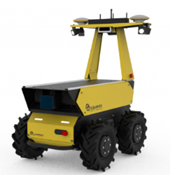
\includegraphics[width=\linewidth]{figures/weijie/4.png}
    \caption{Clearpath Husky UGV}
\end{subfigure}
\hfill
\begin{subfigure}{0.32\linewidth}
    \centering
    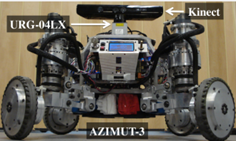
\includegraphics[width=\linewidth]{figures/weijie/5.png}
    \caption{Intel RealSense D435i + RTAB-Map}
\end{subfigure}
\hfill
\begin{subfigure}{0.32\linewidth}
    \centering
    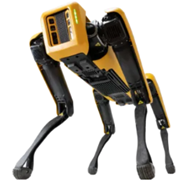
\includegraphics[width=\linewidth]{figures/weijie/6.png}
    \caption{Boston Dynamics Spot}
\end{subfigure}
\caption{Representative SLAM-based robotic platforms discussed in the literature review.}
\label{fig:slam-projects-weijie}
\end{figure}

The literature reveals a clear tradeoff. Multi-sensor or LiDAR-dominant systems usually provide stronger precision, robustness, and engineering maturity, but these benefits come at the cost of higher hardware expense, greater physical size, and more difficult system integration. This is especially important in scenarios where many robots are needed, where scanning must be performed quickly, or where the environment is narrow and cluttered. In such cases, system scalability becomes not only a perception problem but also a cost and deployment problem.

At the same time, lower-cost visual methods have become increasingly attractive because they reduce hardware requirements and can provide rich scene information. Recent monocular depth and visual reconstruction methods suggest that useful 3D structure can be inferred from far simpler sensing hardware than traditional LiDAR-based systems require. However, the literature also indicates several shortcomings that remain directly relevant to this project: monocular reconstruction is less stable geometrically, visual methods are sensitive to scene conditions, and the consistency needed for later fusion and mapping is harder to guarantee. In addition, many existing systems focus either on local reconstruction quality or on exploration strategy, without fully addressing how low-cost perception, map fusion, and multi-robot planning interact in one complete system.

Research on multi-robot exploration further informs this work. Multi-robot systems can improve environmental coverage and reduce total exploration time by parallelizing data collection, but they also introduce coordination costs, conflict handling, redundant coverage, and map-sharing challenges. This means that adding more robots does not automatically translate into proportional gains in efficiency. The literature therefore suggests that the key challenge is not simply to build a low-cost robot or to deploy multiple robots, but to design a system in which perception quality, fusion stability, and planning decisions remain compatible across the whole pipeline.

These observations directly inform the goals of the present project. Rather than trying to compete with high-end SLAM systems in absolute accuracy, this work focuses on a different gap in the literature: how to build a practical, scalable, and low-cost scanning pipeline that remains useful despite weaker sensing hardware. The project therefore combines monocular perception, centralized computation, swarm-style exploration, and map-based planning in order to test whether acceptable reconstruction and exploration performance can still be achieved under stronger cost constraints.

\section{Theoretical, Mathematical and Scientific Background}


\subsection{Relative Pose Estimation of the Robot}
\label{subsec:relative-pose-estimation-zhuyu-dong}

\subsubsection{Coordinate Systems and the Chain Rule}

To estimate the relative position of the robot, multiple reference frames are introduced. In this work, the fixed world reference frame is denoted as the global coordinate system \( \{W\} \), while the coordinate system attached to the robot body is denoted as the local coordinate system \( \{B\} \). The global coordinate system provides a unified reference for describing the robot pose in the environment, whereas the local coordinate system is more suitable for representing short-term motion increments.

The pose of the robot in the global coordinate system can be written as the homogeneous transformation matrix
\[
{}^{W}T_{B}=
\begin{bmatrix}
{}^{W}R_{B} & {}^{W}p_{B} \\
0 & 1
\end{bmatrix}
\]
where \({}^{W}R_{B}\) is the rotation matrix of the robot body frame relative to the global frame, and \({}^{W}p_{B}\) is the position vector of the robot origin in the global frame. If a point \(P\) is represented in the local coordinate system as \({}^{B}p\), then its coordinates in the global coordinate system can be expressed as
\[
{}^{W}p = {}^{W}R_{B}\,{}^{B}p + {}^{W}p_{B}.
\]
This equation shows that a point is first rotated and then translated when transformed from the local frame to the global frame.

To update the pose across consecutive time steps, the chain rule of coordinate transformation is adopted. Let the robot body frames at time \(k-1\) and \(k\) be denoted by \( \{B_{k-1}\} \) and \( \{B_k\} \), respectively. Their relationship can be written as
\[
{}^{W}T_{B_k} = {}^{W}T_{B_{k-1}}\,{}^{B_{k-1}}T_{B_k}.
\]
Here, \({}^{B_{k-1}}T_{B_k}\) represents the local pose increment between two adjacent time steps. Based on this chained relationship, the robot pose can be recursively updated in the global frame, or equivalently represented relative to any chosen reference frame.

\subsubsection{Coordinate Transformation Update Based on Velocity and Attitude}

When the local displacement increment and the previous attitude of the robot are known, the current coordinate transformation can be updated recursively. Let \(\Delta p_{k-1}\) denote the displacement increment in the local frame at time \(k-1\). The robot position in the global coordinate system at time \(k\) can then be computed as
\[
p_k = p_{k-1} + R_{k-1}\Delta p_{k-1},
\]
where \(p_{k-1}\) is the global position vector at the previous time step, and \(R_{k-1}\) is the rotation matrix of the robot body frame relative to the global frame. This equation indicates that the local motion increment must first be rotated into the global frame before being added to the previous position.

The local displacement increment can be approximated from the robot velocity and the sampling interval. If the forward linear velocity is \(v\) and the sampling interval is \(\Delta t\), then
\[
\Delta p_{k-1}=
\begin{bmatrix}
v\Delta t \\
0 \\
0
\end{bmatrix}.
\]
This formulation assumes that the robot motion within one time step mainly occurs along the forward axis of the body frame. In practice, the robot heading may change continuously during motion. Therefore, a smaller \(\Delta t\) usually leads to better consistency between the assumed motion direction and the actual attitude, which improves the accuracy of the estimated position.

Using this recursive formulation together with the chain rule, the robot pose can be expressed not only in the global frame but also relative to any selected reference frame. However, since this method depends on the commanded velocity, the sampling interval, and the attitude measurement result, the estimation error accumulates over time. Therefore, external position feedback or other correction information should be introduced periodically to suppress long-term drift.

\subsection{Image-to-Point Cloud Reconstruction}
\label{subsec:image-to-point-cloud-junjie-ouyang}

\subsubsection{Monocular Depth Estimation}
\label{subsubsec:monocular-depth-estimation-junjie-ouyang}

This work is based on monocular depth estimation and camera projection geometry. The aim of this submodule is to recover a usable point cloud from a single RGB image. This is important because the point cloud is later used for fusion, mapping, and path planning in the full team system.

Monocular depth estimation predicts scene depth from one image~\cite{godard2019}. A single RGB image only records the 2D appearance of a scene. It contains colour, brightness, texture, edges, and object shapes, but it does not directly provide real 3D distance. In other words, the image shows how the scene looks on the image plane, not how far each point is from the camera in physical space. The depth of each pixel must therefore be inferred from visual cues such as perspective, occlusion, scale, texture variation, and object structure. For example, objects that appear smaller may be farther away, and strong perspective lines may suggest depth change across a surface. However, these cues are indirect, so the problem is difficult and often ambiguous. Different real 3D scenes can produce similar 2D image patterns. Even so, monocular depth estimation is attractive for low-cost robotic systems because it only requires one camera. This reduces hardware cost, weight, and system complexity.

\subsubsection{Relative Depth and Metric Depth}
\label{subsubsec:relative-metric-depth-junjie-ouyang}

A key idea in this area is the difference between relative depth and metric depth. Relative depth mainly describes the order of depth in a scene. It can show which parts are closer and which parts are farther away, but the numerical values do not necessarily match real physical distance. Metric depth, by contrast, tries to produce values that are more consistent with true scene geometry. Recent monocular depth models such as Depth Anything V2 and Depth Pro reflect this broader move toward stronger generalisation and more practical geometric output~\cite{yang2024,bochkovskii2024}. For this project, this distinction is important because the depth map is not the final result. It must be converted into a point cloud and then passed to later modules. If the depth is only correct in a relative sense, the reconstructed point cloud may still have incorrect scale and distance even if the shape looks visually reasonable. This would reduce its value for later geometric processing such as point cloud fusion and map construction.

\subsubsection{Pinhole Camera Model}
\label{subsubsec:pinhole-camera-model-junjie-ouyang}

The conversion from a depth map to a point cloud is based on the pinhole camera model~\cite{hartley2004}. This model describes how a 3D scene is projected onto a 2D image plane through a camera. In this model, each image pixel corresponds to a ray that starts at the camera centre and passes through the image plane. If the depth value of a pixel is known, the 3D position of the corresponding scene point can be recovered along that ray. This is why depth estimation and camera geometry must be considered together. The basic geometry of the pinhole camera model is illustrated in Fig.~\ref{fig:camera-model-junjie}. The camera intrinsics define how image coordinates relate to directions in 3D space. These intrinsics include the focal lengths in the horizontal and vertical directions, denoted by $f_x$ and $f_y$, and the principal point, denoted by $(c_x,c_y)$, which represents the optical centre of the image.

\begin{figure}[htbp]
    \centering
    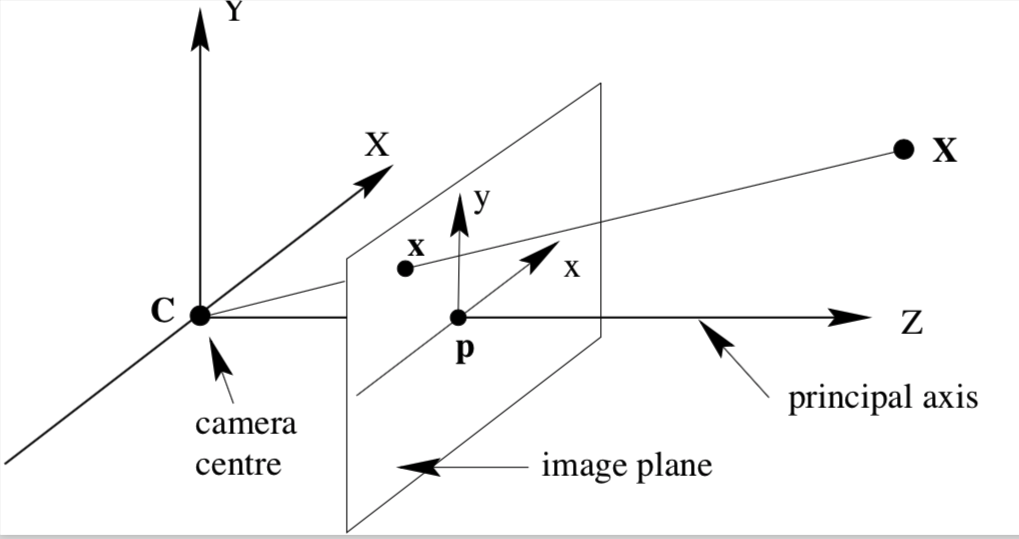
\includegraphics[width=0.72\textwidth]{figures/junjie/camera.png}
    \caption{Geometry of the pinhole camera model.}
    \label{fig:camera-model-junjie}
\end{figure}

\subsubsection{Back-Projection Geometry}
\label{subsubsec:back-projection-geometry-junjie-ouyang}

Let $(u,v)$ be the image coordinates of a pixel and let $Z$ be its depth. If the focal lengths are $f_x$ and $f_y$, and the principal point is $(c_x,c_y)$, the corresponding 3D point $(X,Y,Z)$ in the camera coordinate system can be written as
\[
X = \frac{(u-c_x)Z}{f_x}, \qquad
Y = \frac{(v-c_y)Z}{f_y}, \qquad
Z = Z.
\]
These equations describe the back-projection process. The term $(u-c_x)$ gives the horizontal offset of the pixel from the optical centre, and $(v-c_y)$ gives the vertical offset. Dividing by focal length converts these image offsets into normalised camera coordinates. Multiplying by $Z$ then scales the point to its position in 3D space. In this way, the depth value controls how far the point lies from the camera, while the pixel position determines its lateral location. This back-projection step is the main mathematical link between the depth map and the final point cloud.

\subsubsection{Camera Calibration}
\label{subsubsec:camera-calibration-junjie-ouyang}

The quality of the reconstructed point cloud also depends on camera calibration~\cite{zhang2000}. A real camera does not perfectly follow the ideal pinhole model. Lens distortion changes the relationship between image position and the true viewing ray. If the intrinsic parameters are inaccurate, or if distortion is not handled properly, the reconstructed 3D points will contain systematic geometric error. This means that even if the depth prediction is reasonable, the final point cloud may still show incorrect shape, position, or scale. For this reason, calibration is important for improving geometric consistency in single-image point cloud reconstruction.

\subsection{Point Clould Merging}
\label{subsec:surface-fusion-qingzhou-zhang}

\subsubsection{Registration}

Due to technical limitations, robotic control systems are unable to provide perfectly accurate initial poses for point clouds. Therefore, a registration step is required before merging individual point clouds. Point cloud registration refers to estimating a spatial transformation that aligns multiple point clouds into a common reference coordinate system.
\begin{figure}[htbp]
    \centering
    \begin{subfigure}[b]{0.49\linewidth}
        \centering
        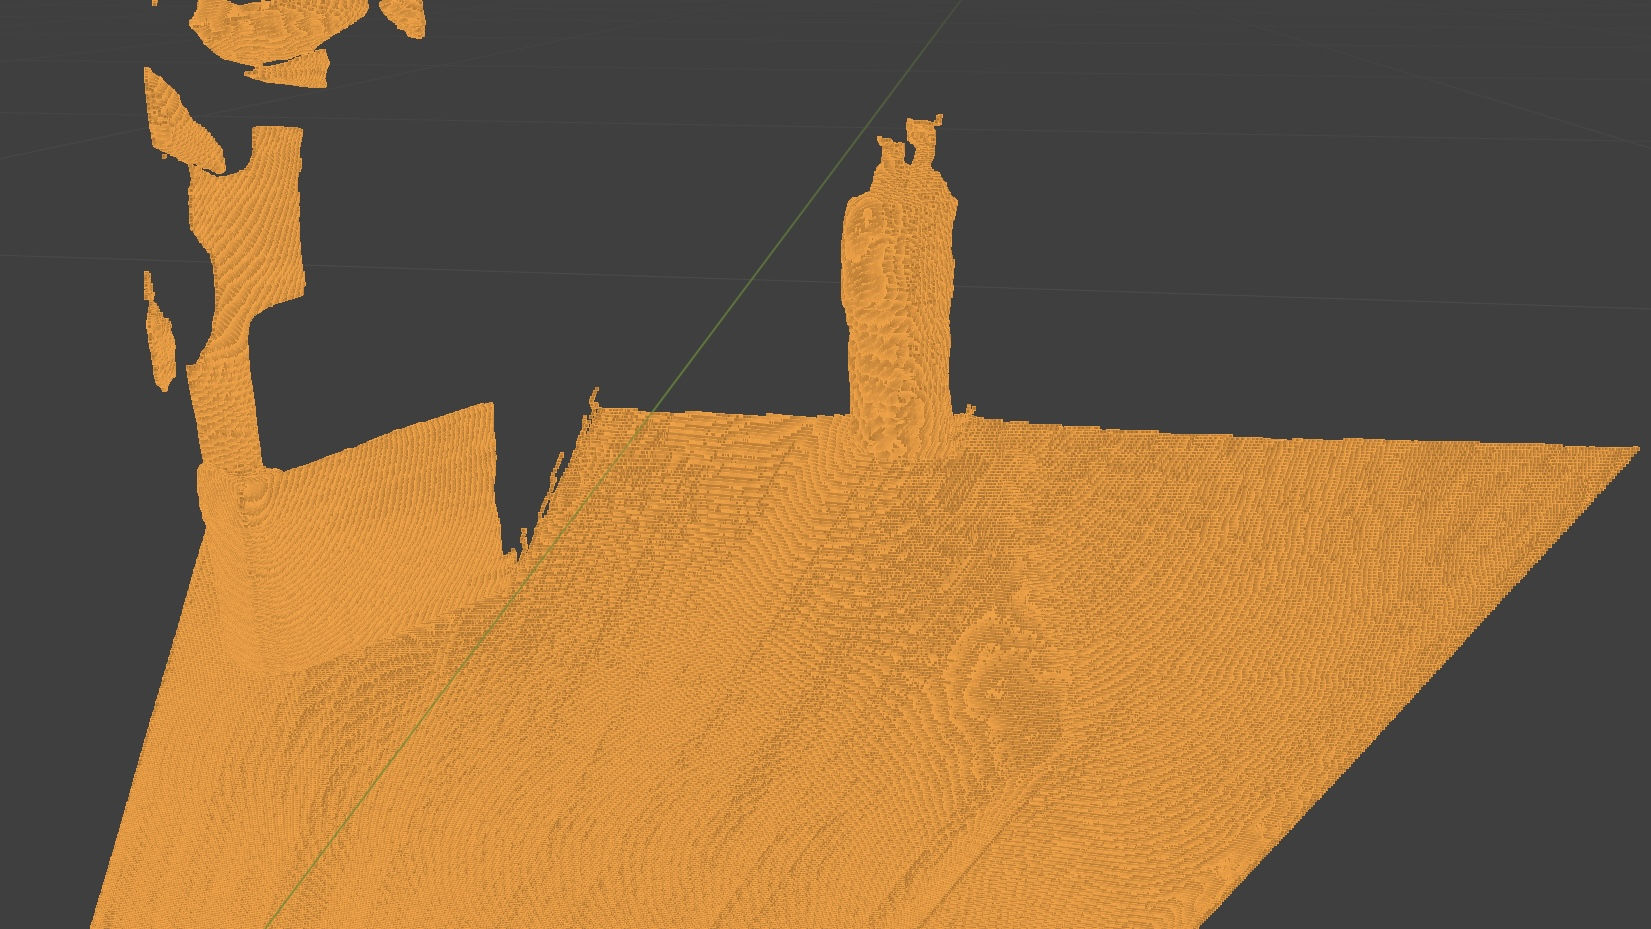
\includegraphics[width=\linewidth]{figures/qingzhou/before_registration_1.jpg}
    \end{subfigure}
    \hfill
    \begin{subfigure}[b]{0.49\linewidth}
        \centering
        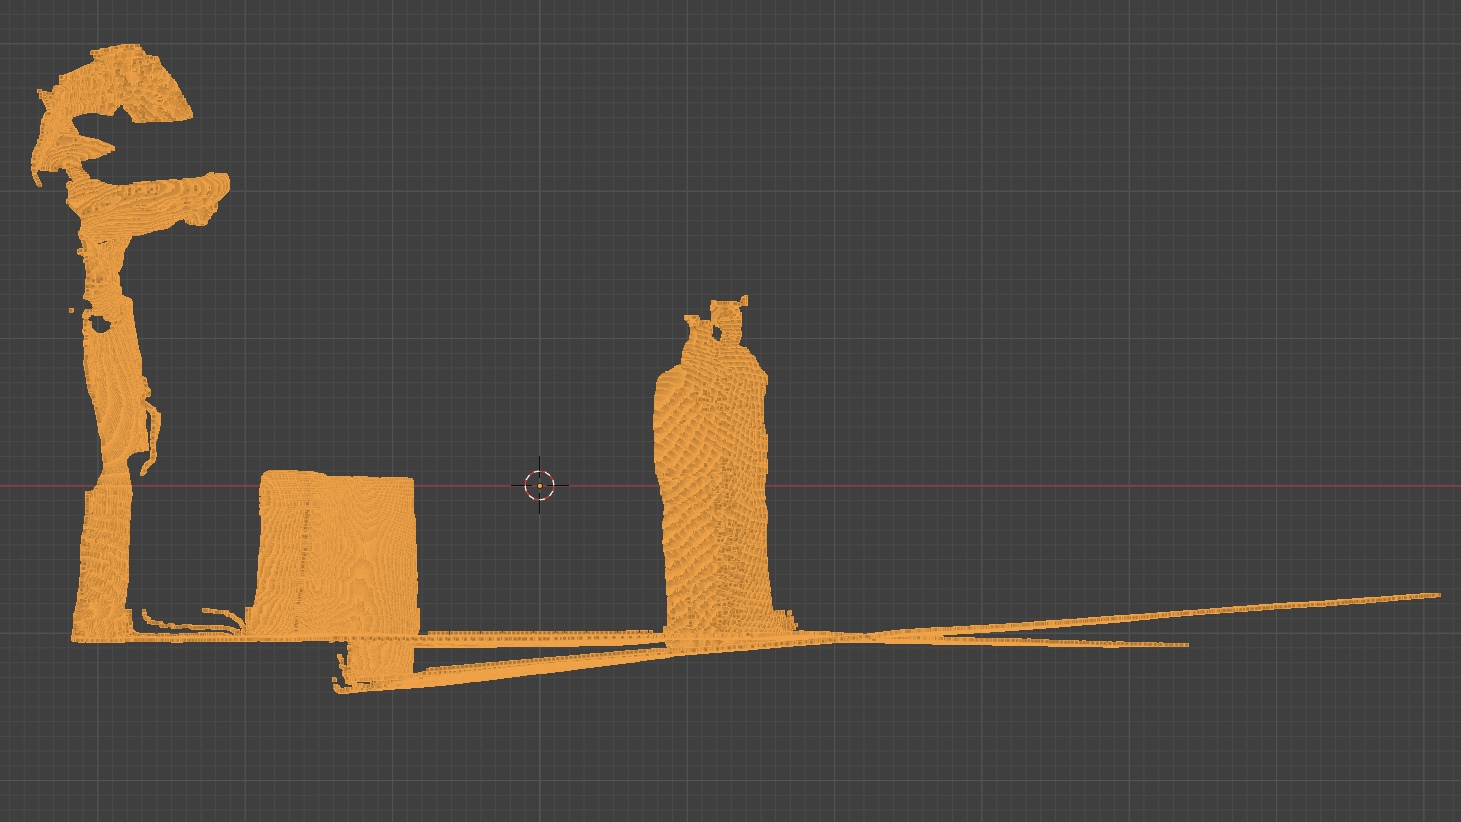
\includegraphics[width=\linewidth]{figures/qingzhou/before_registration_2.jpg}
    \end{subfigure}
    \caption{Merged result only based on initial pose.}
    \label{fig:before-registration-qingzhou}
\end{figure}
The most fundamental method for point cloud registration is the Iterative Closest Point (ICP) algorithm~\cite{besl1992icp}. The core idea of ICP is to iteratively perform nearest-neighbour correspondence matching and rigid transformation estimation, gradually minimizing the alignment error between two point clouds. Given a source point cloud $\mathcal{P}$ and a target point cloud $\mathcal{Q}$, ICP establishes correspondences and minimizes the following objective function:

\begin{equation}
E(R, t) = \sum_{i} \| q_i - (R p_i + t) \|^2
\end{equation}

where $R$ and $t$ represent the rotation and translation, respectively. This problem is typically solved efficiently using Singular Value Decomposition (SVD), and the algorithm converges iteratively to a local optimum.

In this project, the input point cloud is reconstructed from monocular images using an AI model. The primary errors in such point clouds include depth noise along the viewing direction and local geometric distortions, such as scale drift and structural stretching. Under these conditions, ICP becomes unsuitable because it implicitly assumes isotropic Gaussian noise, that is, the covariance satisfies $\Sigma = \sigma^2 I$. However, in monocular reconstruction, uncertainty along the depth direction is significantly larger than in the tangential directions, resulting in strongly anisotropic error distributions. Consequently, ICP assigns excessive weight to depth errors, leading to systematic bias in the optimization results.

In contrast, the Generalized Iterative Closest Point (GICP) algorithm~\cite{segal2009gicp} introduces local covariance modelling to address this issue. GICP represents each point as a Gaussian distribution incorporating local geometric structure and minimizes the Mahalanobis distance:

\begin{equation}
E(R, t) = \sum_{i} (q_i - (R p_i + t))^T (C_i^p + R C_i^q R^T)^{-1} (q_i - (R p_i + t))
\end{equation}

This formulation allows deviations within local geometric structures without being penalized as large errors. Therefore, GICP avoids over-amplifying depth noise and significantly improves both stability and accuracy of registration in this project.

\subsubsection{Surface Fusion}

When constructing a 3D map from multiple frames of point clouds, simply stacking registered point clouds often leads to noise accumulation and surface discontinuities. Therefore, a robust surface representation method is required to consistently integrate multiple observations.
\begin{figure}[htbp]
    \centering
    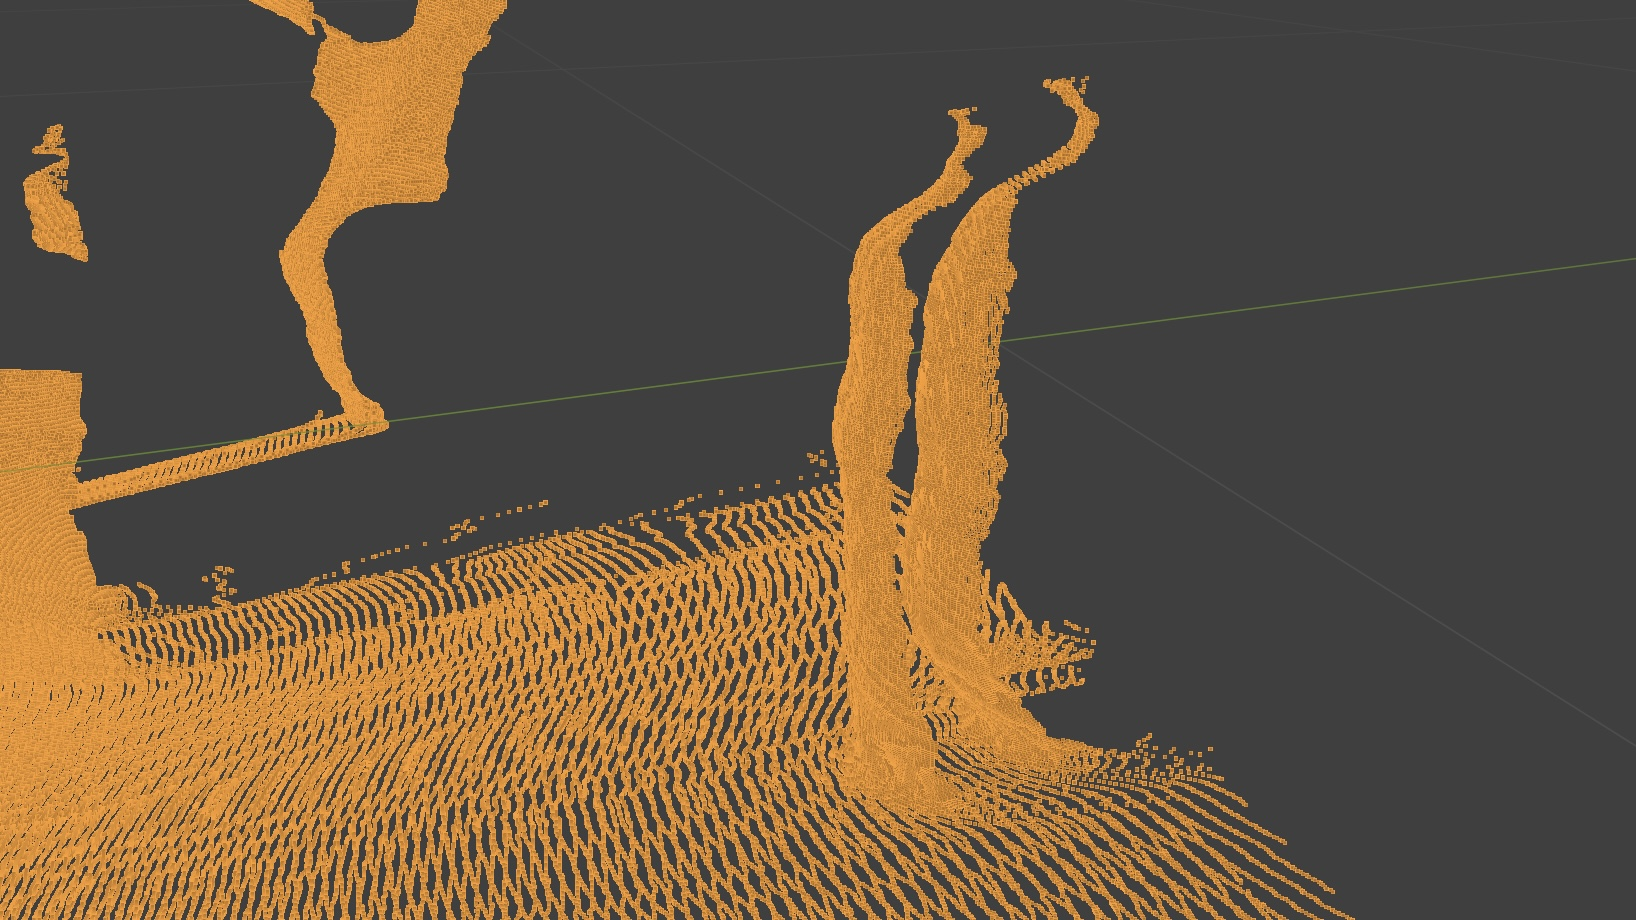
\includegraphics[width=\linewidth]{figures/qingzhou/before_fusion.jpg}
    \caption{Merged result without surface fusion.}
    \label{fig:before-fusion-qingzhou}
\end{figure}
In this project, a surfel-based representation~\cite{pfister2000surfels} is adopted. A surfel (surface element) approximates a local surface region and typically contains attributes such as position, normal vector, colour, and a confidence weight representing observation reliability. Compared to discrete point representations, surfels incorporate local geometric structure, enabling progressive refinement of surface estimates across multiple observations and improving smoothness and consistency.

Surface fusion can be formulated as an incremental update problem. For each new frame, correspondences between observations and existing surfels must be established, followed by updating surfel attributes. Data association is typically based on geometric and photometric consistency measures, such as position, normal direction, and colour similarity.

For matched observations, the fusion process usually follows a weighted update scheme:

\begin{equation}
A_{\text{new}} = \frac{w_{\text{old}} A_{\text{old}} + w_{\text{obs}} A_{\text{obs}}}{w_{\text{old}} + w_{\text{obs}}}
\end{equation}

where $A$ denotes a surfel attribute, such as position or color, and $w$ represents the confidence weight. This formulation can be interpreted as a recursive estimation process, allowing surfel attributes to converge to stable values over multiple observations. For observations that cannot be matched to existing surfels, new surfels are introduced to expand the map representation.

Additionally, maintenance operations are required to ensure long-term map stability, such as merging redundant surfels and removing unreliable ones.

Overall, surfel-based surface fusion effectively integrates noisy multi-frame observations while preserving local geometric structure, making it particularly suitable for scenarios with unstable input quality.

\subsection{2D Map Generation and Cost Modeling}
\label{subsec:2dmap-theory-zhuyu-dong}

\subsubsection{Two-Dimensional Grid Map and Its Role}

To use a 3D point cloud for subsequent route search and path planning, the environment is first discretized into a two-dimensional grid map~\cite{elfes1989occupancy}. The space is divided into regular cells with a fixed resolution, and each cell represents a local region of the environment. In this way, the originally continuous and large-scale point cloud is compressed into a regular discrete representation.

The main role of the 2D grid map is to provide a discretized search space for path-planning algorithms. Direct search on the raw point cloud is computationally expensive because the data scale is large and the adjacency relationship among points is complicated. After grid discretization, path search only needs to be performed among a finite number of cells, which makes the neighborhood relationship clearer and reduces the computational burden~\cite{elfes1989occupancy,gu2008traversability}.

In addition, the 2D grid map helps control the growth of complexity as the map becomes larger. Local geometric information in each region can be summarized by a traversal cost \(cost\), where a larger value indicates more difficult traversal and a smaller value indicates better traversability. In this way, the environment is represented as a collection of cost-associated cells, which provides a compact and efficient input for subsequent path planning.

\subsubsection{Ground Layer Selection}

During the construction of a two-dimensional grid map, a single grid cell may contain more than one layer of points. In addition to the actual ground, points may also come from the bottom of obstacles, suspended structures, or noise. Therefore, the lowest point in a cell cannot be directly regarded as the ground. To address this issue, candidate layers are first constructed along the vertical direction in each grid cell, and then the layer that most likely represents the actual ground is selected~\cite{meng2018terrain}.

Let the candidate layer set of the \(i\)-th grid cell be
\[
\mathcal{L}_i = \{L_{i,1}, L_{i,2}, \dots, L_{i,m_i}\}
\]
where \(m_i\) is the number of candidate layers in the cell. For each candidate layer \(L_{i,k}\), its representative height is defined as
\[
h_{i,k} = \frac{1}{N_{i,k}} \sum_{p \in L_{i,k}} y(p)
\]
where \(N_{i,k}\) is the number of points in \(L_{i,k}\), and \(y(p)\) is the height coordinate of point \(p\).

Since the actual ground is usually locally continuous, ground-layer selection should depend not only on the height distribution inside the current cell but also on the ground height of neighboring cells~\cite{meng2018terrain,gu2008traversability}. Let \(\hat{h}_{\mathcal{N}(i)}\) denote the reference ground height in the neighborhood of the \(i\)-th cell. Then the ground layer of the current cell can be defined as
\[
L_i^\ast = \arg\min_{L_{i,k} \in \mathcal{L}_i}
\left| h_{i,k} - \hat{h}_{\mathcal{N}(i)} \right|
\]
which means that the candidate layer whose height is closest to the neighborhood reference ground height is selected as the ground layer. To avoid incorrectly classifying a layer with a large height difference as ground, an additional continuity constraint can be introduced:
\[
\left| h(L_i^\ast) - \hat{h}_{\mathcal{N}(i)} \right| < \tau_h
\]
where \(\tau_h\) is the ground-continuity threshold. This candidate-layer selection strategy based on neighborhood continuity can extract the actual ground more robustly and reduce the interference caused by suspended structures, obstacle boundaries, and local noise.

\subsubsection{Eigenvalues and Eigenvectors for Geometric Characteristics}

After ground-layer selection, the local geometric characteristics of each grid cell still need to be analyzed in order to evaluate traversability. In this work, eigen-analysis is not performed on the entire map as a whole. Instead, it is carried out separately for each grid cell by constructing a covariance matrix from its local point set~\cite{weinmann2013feature}. As a result, the obtained eigenvalues and eigenvectors describe the local surface properties of each individual cell rather than the global properties of the entire map.

For the \(i\)-th grid cell, let its local point set be
\[
\mathcal{P}_i = \{p_1, p_2, \dots, p_{N_i}\}, \quad p_k \in \mathbb{R}^3
\]
and let its centroid be
\[
\bar{p}_i = \frac{1}{N_i}\sum_{k=1}^{N_i} p_k
\]
Then the covariance matrix of this cell is defined as
\[
C_i = \frac{1}{N_i}\sum_{k=1}^{N_i}(p_k-\bar{p}_i)(p_k-\bar{p}_i)^T
\]
The eigen-decomposition of \(C_i\) is written as
\[
C_i n_{i,j}=\lambda_{i,j} n_{i,j}, \quad j=1,2,3
\]
with
\[
\lambda_{i,1}\le \lambda_{i,2}\le \lambda_{i,3}
\]

If the local point set in the cell is approximately distributed on a plane, then the eigenvector corresponding to the smallest eigenvalue, \(n_{i,1}\), can be regarded as the approximate normal vector of the local ground surface~\cite{weinmann2013feature}. Let the unit vertical direction be
\[
v=
\begin{bmatrix}
0\\
0\\
1
\end{bmatrix}
\]
This eigenvector can also be treated as the surface orientation vector for slope evaluation. Then the local slope of the cell can be expressed as
\[
\theta_i=\arccos\left(\frac{n_{i,1}\cdot v}{\|n_{i,1}\|\,\|v\|}\right)
\]
where a larger \(\theta_i\) indicates a larger local surface inclination.

At the same time, the smallest eigenvalue \(\lambda_{i,1}\) reflects the dispersion of points along the normal direction and can therefore be used to characterize the local roughness or unevenness of the cell. A normalized roughness index can be defined as
\[
r_i=\frac{\lambda_{i,1}}{\lambda_{i,1}+\lambda_{i,2}+\lambda_{i,3}}
\]
where a larger \(r_i\) indicates a rougher or less stable local surface.

\begin{figure}[htbp]
\centering
\begin{subfigure}[b]{0.47\columnwidth}
    \centering
    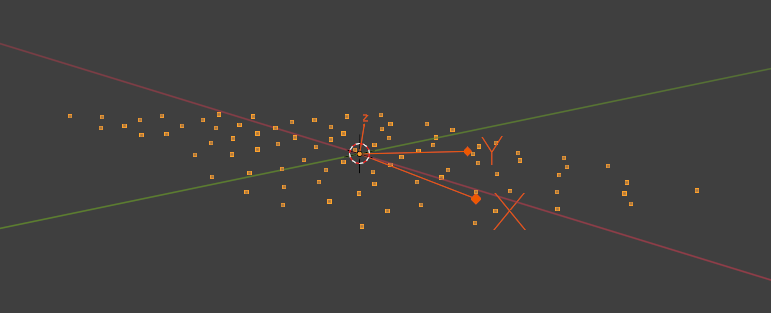
\includegraphics[width=\columnwidth]{figures/smallev.png}
    \caption{Cell with smaller minimum eigenvalue.}
    \label{fig:smallev}
\end{subfigure}
\hfill
\begin{subfigure}[b]{0.47\columnwidth}
    \centering
    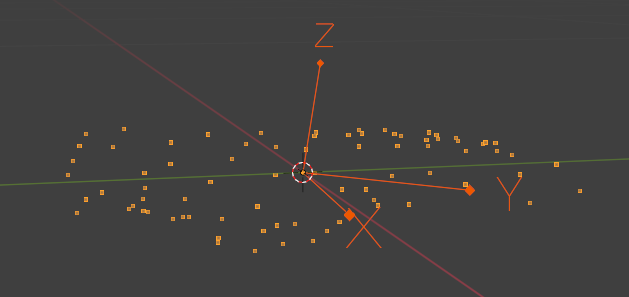
\includegraphics[width=\columnwidth]{figures/bigev.png}
    \caption{Cell with larger minimum eigenvalue.}
    \label{fig:bigev}
\end{subfigure}
\caption{cells with different minimum eigenvalues.}
\label{fig:eigenvalue-comparison}
\end{figure}

Therefore, the eigenvector associated with the smallest eigenvalue mainly describes the local directional property of each grid cell, while the smallest eigenvalue itself reflects the stability of the cell along the surface normal direction. By analyzing slope and roughness on a cell-by-cell basis, the local traversability of different regions can be quantified and used for subsequent cost-map construction. As illustrated in Fig.~\ref{fig:eigenvalue-comparison}, two cells may exhibit similar slope angles while still having different roughness levels. The annotated \(z\)-vector in each figure corresponds to the eigenvector associated with the smallest eigenvalue, and the angle between this vector and the world \(z\)-axis represents the local slope, which is approximately \(17^\circ\) in both cases. Compared with Fig.~\ref{fig:smallev}, the cell in Fig.~\ref{fig:bigev} contains a local pit and is therefore geometrically more irregular, leading to a larger minimum eigenvalue.

\subsection{Path Planning}
\label{subsec:path-planning-theory-weijie-chen}

\subsubsection{Map Representation and Frontier Definition}

This project uses a two-dimensional occupancy grid to represent the environment:
\[
m_{i,j} \in \{-1,0,1\}
\]
where \(-1\) denotes UNKNOWN, \(0\) denotes FREE, and \(1\) denotes OCCUPIED. On this basis, a frontier is defined as
\[
\textit{Frontier} = \{(i,j)\mid m_{i,j} = \textit{FREE},\ \exists\ \textit{neighbour} = \textit{UNKNOWN}\}.
\]
That is, a frontier cell is traversable itself and is adjacent to at least one unknown cell.

\subsubsection{Robot Motion and Coordinate Model}

The robot moves in continuous space, and its state is represented as
\[
s = (x, z, \theta)
\]
where \(\theta\) is the orientation angle. The motion direction is determined by
\[
\Delta r = \cos(\theta), \quad \Delta c = \sin(\theta),
\]
and the update rule is
\[
r_{t+1} = r_t + \Delta r \cdot d, \quad c_{t+1} = c_t + \Delta c \cdot d,
\]
where \(d\) represents the distance moved.

\subsubsection{Path Planning Method (\(A^*\))}

Path planning uses the \(A^*\) algorithm with
\[
f(n) = g(n) + h(n), \qquad h(n) = |x_n - x_g| + |y_n - y_g|.
\]
To incorporate environmental risk into the path cost, the cost function is extended as
\[
g(n) = g(n-1) + 1 + \lambda \cdot cost(n).
\]
This allows the planner to prefer shorter paths while also avoiding high-risk areas.

\subsubsection{Collision Detection Model}

The robot is modeled as a circle whose feasible region satisfies
\[
(x - x_0)^2 + (y - y_0)^2 \le r^2
\]
where \(r\) is the robot radius. During pathfinding, the path is sampled continuously, and all sampled points must remain in traversable space for the path to be considered safe.

\subsubsection{Perception Models and Information Acquisition}

The robot uses an FOV model for perception:
\[
\theta \in \left[ \theta_0 - \frac{\textit{FOV}}{2},\ \theta_0 + \frac{\textit{FOV}}{2} \right].
\]
The number of visible unknown cells within the field of view is
\[
U = \sum 1_{\textit{cell} = \textit{UNKNOWN}}.
\]
This helps guide the robot toward directions with greater potential information gain.

\subsubsection{Observation Overlap Constraint}

To ensure adjacent observations can be fused, an overlap constraint is introduced:
\[
\textit{Overlap} = \frac{\textit{FOV} - |\Delta \theta|}{\textit{FOV}}.
\]
To preserve sufficient overlap between neighboring observations, the planner enforces
\[
\textit{Overlap} \ge \textit{min\_overlap\_ratio}.
\]

\subsubsection{Single-Robot Decision-Making Model}

The robot selects targets using a composite scoring function:
\[
\textit{Score} = \textit{Path}_{length} + \textit{Yaw}_{penalty} + \textit{Cost}_{penalty} + \textit{Overlap}_{penalty} - \textit{Unknown}_{gain}.
\]
Here, path length, turning cost, and environmental risk are treated as penalties, while newly observable unknown area is treated as gain. The robot selects the target with the lowest score.

\subsubsection{Multi-Robot Collision Avoidance}

In the multi-robot setting, collision avoidance is enforced through position and distance constraints:
\[
(x_i, y_i) \neq (x_j, y_j), \qquad d(r_i, r_j) > d_{\min}.
\]

\subsubsection{Field-of-View Constraints and Cooperative Avoidance}

When one robot may enter the field of view of another,
\[
r_j \in \textit{FOV}_i,
\]
the corresponding area is treated as forbidden during planning:
\[
M_{plan} = M \setminus \textit{Forbidden}.
\]
This helps reduce visual interference and improves cooperative exploration stability.



\section{Methods, Setups and Software Implementation}

\subsection{Architecture Overview}
\label{subsec:swarm-centralized-architecture-zhuyu-dong}

This work adopts a swarm-based scanning strategy, in which multiple robots scan the environment in parallel. Compared with a single-robot solution that scans the scene region by region, this approach can collect environmental information over a larger area within a shorter time. Meanwhile, the number of deployed robots can be adjusted according to the environment size and practical constraints such as time and cost, which makes the overall scheme more flexible.

\begin{figure}[htbp]
    \centering
    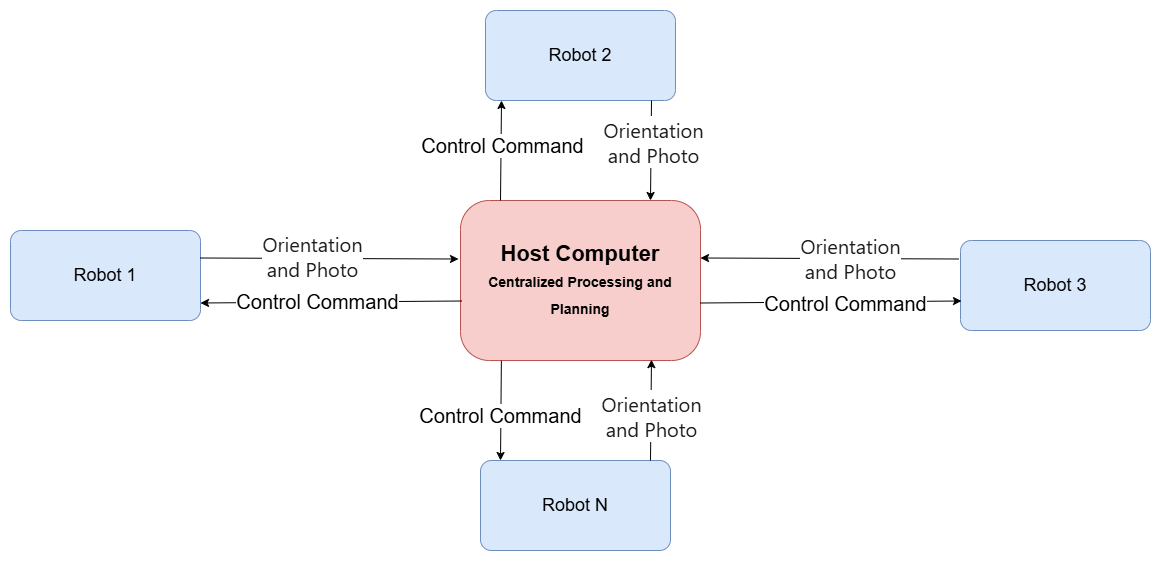
\includegraphics[width=0.95\columnwidth]{figures/Centralized processing architecture for swarm monocular SLAM robots.png}
    \caption{Centralized processing architecture for swarm monocular SLAM robots.}
    \label{fig:centralized-architecture}
\end{figure}

Since AI-based models are used in the subsequent processing stages, the system requires relatively high computing power. However, if every individual SLAM robot were equipped with a high-performance NPU or other dedicated AI hardware, the total hardware cost in a multi-robot scenario would increase significantly, as shown in Fig.~\ref{fig:centralized-architecture}. To reduce this cost, a centralized data-processing architecture is adopted. Under this architecture, all SLAM robots are treated as executors and sensors. Their onboard functions are limited to motion, image acquisition, and pose-related data collection, while computationally intensive AI inference is not performed locally. Instead, all collected data are transmitted through the network to a high-performance host computer, which is responsible for unified data processing, map construction, and path planning. In this way, the high computational load is concentrated on a single terminal, effectively reducing the hardware cost of each robot.

\begin{figure}[htbp]
    \centering
    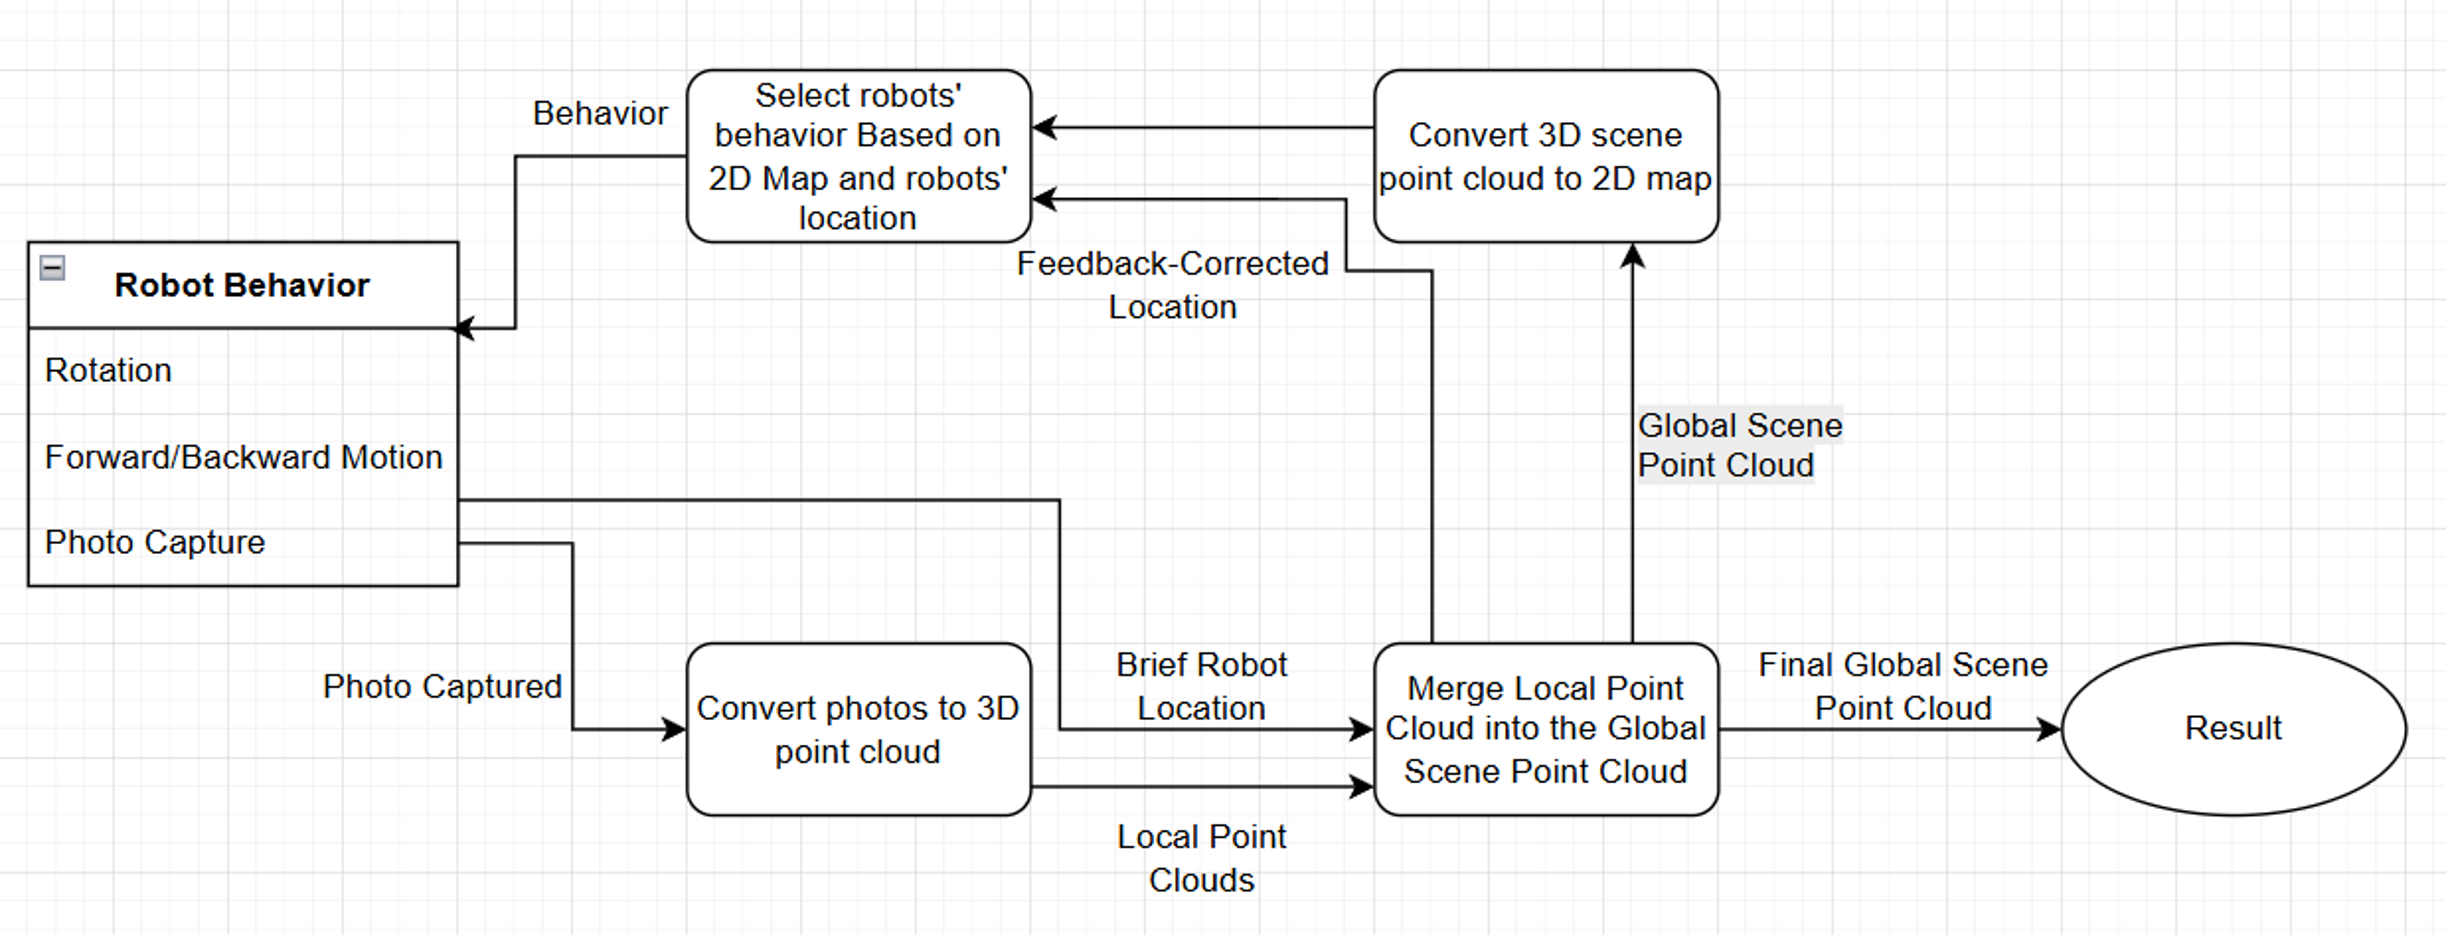
\includegraphics[width=0.95\columnwidth]{figures/overview flow chat.png}
    \caption{Overview flow chart of single-robot control and data acquisition.}
    \label{fig:overview-flow}
\end{figure}


The overall operation flow is shown in Fig.~\ref{fig:overview-flow}. After the host computer receives the images and coarse pose estimates uploaded by the robots, it first applies Depth Pro to convert the images into depth maps, and then reconstructs the point cloud corresponding to each image. Based on the coarse pose estimates, the host computer performs post-processing on each point cloud and merges it into the global point cloud. At the same time, the current robot pose can be further refined using the feedback from the merging error, so that a more accurate pose estimate is obtained. On this basis, the global point cloud is further converted into a 2D map, which is used to determine traversable regions, blocked regions, unexplored regions, and the traversal cost of different areas. The path-planning module then generates paths and motion commands for each robot according to the refined poses and the current 2D map. When all robots have completed the scanning task, that is, when no further valid path can be planned, the scanning process ends. Finally, the merged global point cloud is exported as the output of the complete scanning task.


\subsection{Robot Platform}
\label{subsec:robot-platform-zhuyu-dong}

The robot hardware used in this project was developed through two design iterations. The first-generation platform was built to validate the overall feasibility of monocular image capture, motion control, and pose-related feedback on a compact mobile platform. Based on the practical limitations observed in that prototype, a second-generation robot was then developed and adopted as the final hardware platform of the system. The final platform is a compact and highly integrated robot with a size of approximately \(10 \times 10 \times 10\text{ cm}\), and includes image acquisition, wireless communication, motion execution, and coarse pose estimation capabilities. It uses an \texttt{ESP32-CAM} controller, an \texttt{OV3660} camera, an \texttt{MPU6050} IMU, and a motor-driving structure based on \texttt{L298N} and \texttt{N15} geared DC motors~\cite{espressif_esp32_hwref,invensense_mpu6050,st_l298}. This design preserves the minimum hardware functions required by the system while keeping the robot small and low-cost.

\subsubsection{Second-Generation Platform}
\label{subsubsec:second-generation-platform-zhuyu-dong}
\label{subsec:second-generation-robot-zhuyu-dong}

To address the limitations of the first-generation platform in size, power consumption, stability, and pose estimation accuracy, a second-generation robot was developed and finally adopted in this work. The size was reduced to approximately \(10 \times 10 \times 10\text{ cm}\), which better satisfied the project requirements for miniaturization and low cost. The detailed hardware design of the first-generation robot is provided in Appendix~\ref{app:hardware-iteration}. The second-generation robot adopted \texttt{ESP32-CAM} as the main controller. This chip provides relatively strong performance in a compact form factor while also integrating Wi-Fi communication and a camera interface, which makes it well suited for this project~\cite{espressif_esp32_hwref}. Although the number of available pins is limited, the hardware requirements of the system can still be satisfied by reusing several special-purpose pins.

\begin{figure}[h]
    \centering
    \begin{subfigure}[b]{0.3\columnwidth}
        \centering
        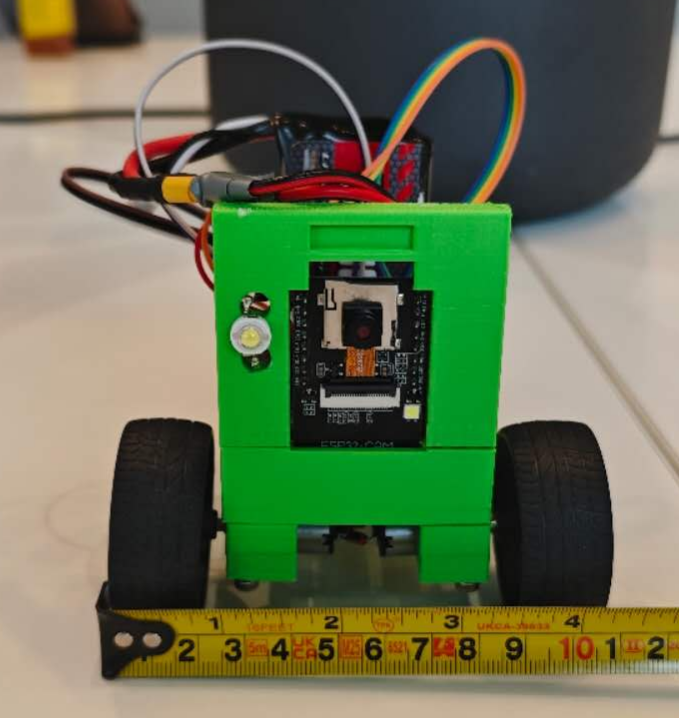
\includegraphics[width=\columnwidth]{figures/car/front.jpg}
        \caption{Front view.}
        \label{fig:car-v2-front-main}
    \end{subfigure}
    \hfill
    \begin{subfigure}[b]{0.3\columnwidth}
        \centering
        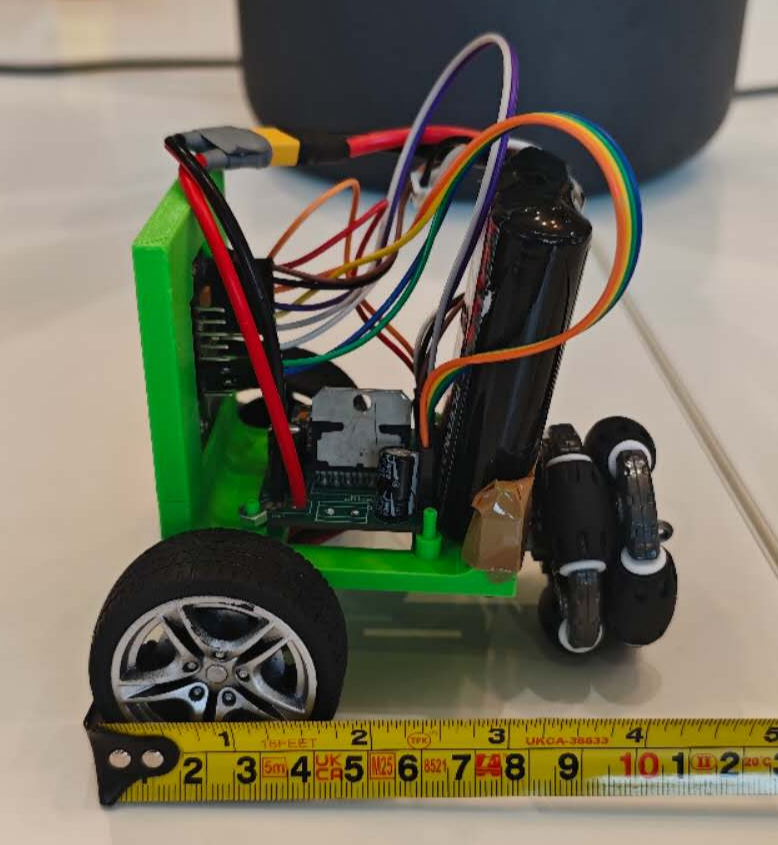
\includegraphics[width=\columnwidth]{figures/car/side.jpg}
        \caption{Side view.}
        \label{fig:car-v2-side-main}
    \end{subfigure}
    \hfill
    \begin{subfigure}[b]{0.3\columnwidth}
        \centering
        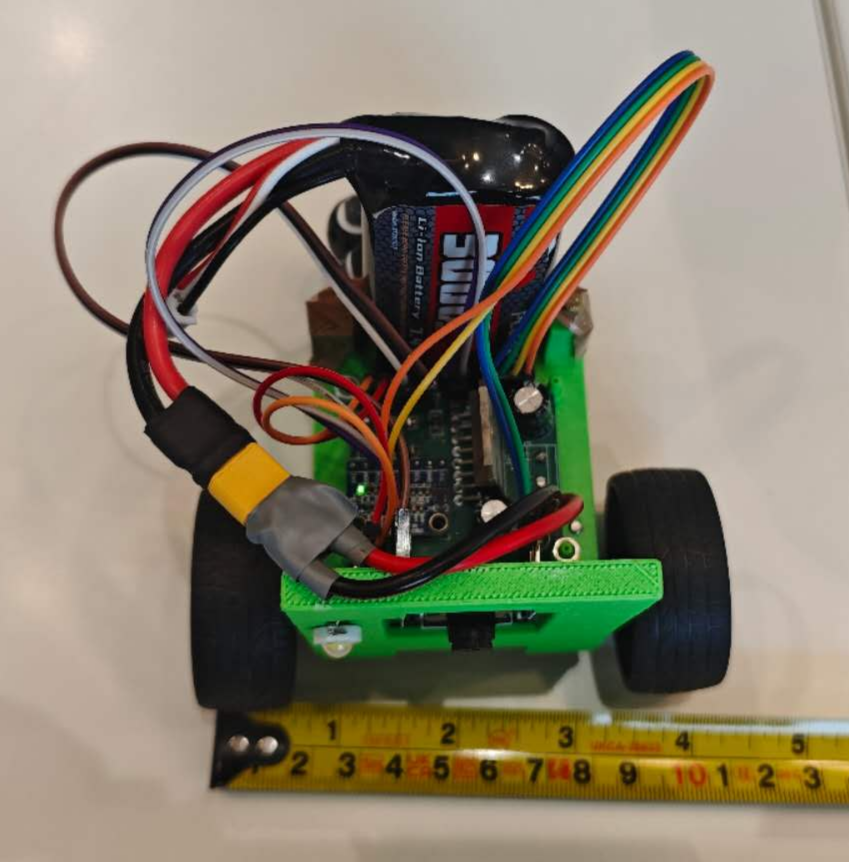
\includegraphics[width=\columnwidth]{figures/car/up.jpg}
        \caption{Top view.}
        \label{fig:car-v2-top-main}
    \end{subfigure}
    \caption{Three-view images of the second-generation robot platform.}
    \label{fig:car-v2-views-main}
\end{figure}

\begin{figure}[h]
    \centering
    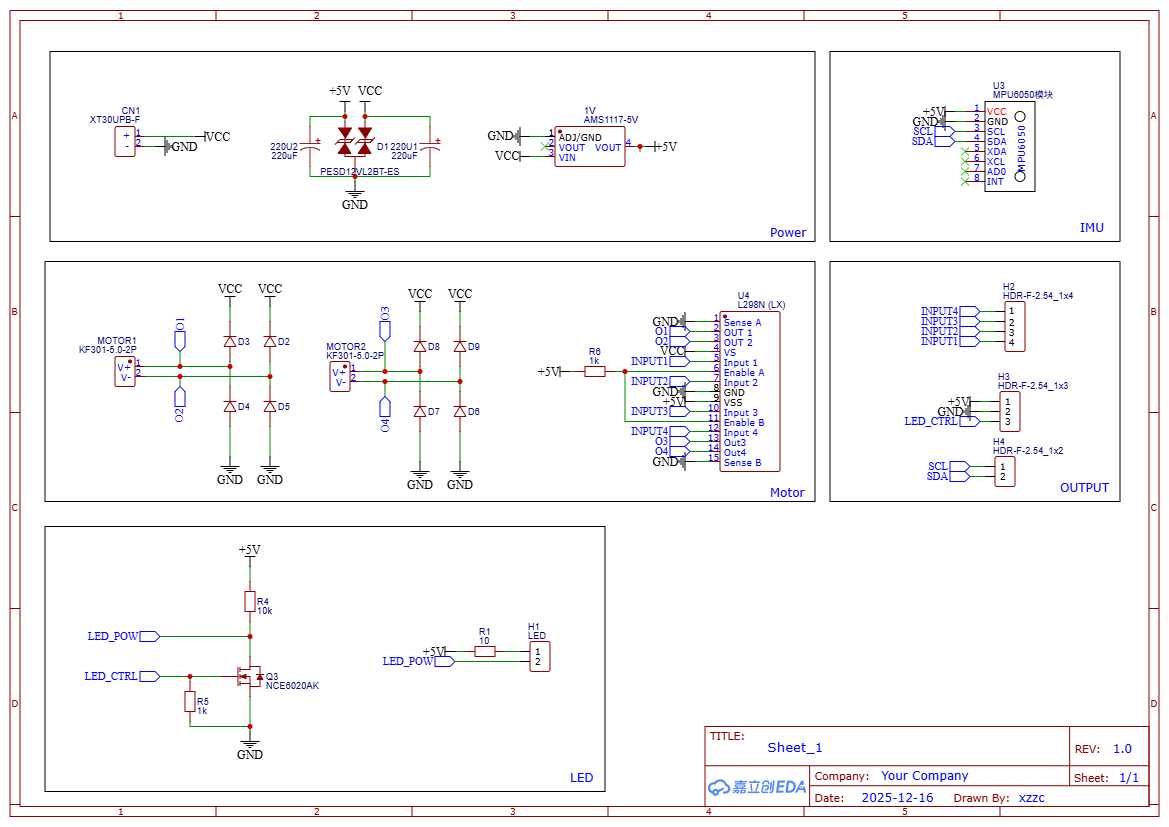
\includegraphics[width=1\columnwidth]{figures/car/V2_sch.png}
    \caption{Circuit schematic of the second-generation robot.}
    \label{fig:car-v2-sch}
\end{figure}

In the camera module, \texttt{OV3660} was selected because it supports a resolution of \(1024 \times 768\), which is close to the effective input scale of Depth Pro and therefore helps reduce unnecessary stretching loss or compression loss. Its field of view is about \(45^\circ\), and lens distortion is small, which allows a relatively large scanning range without introducing strong geometric distortion. In addition, image capture is performed using the \texttt{OV3660} together with LED illumination. For motion, the second-generation robot uses an \texttt{L298N} motor driver together with \texttt{N15} DC geared motors, two rubber drive wheels, and a rear omni-wheel for support and rotation assistance~\cite{st_l298}. Compared with the stepper-motor-based first-generation design, this arrangement provides better speed, stability, and resistance to slipping. The robot realizes forward motion, backward motion, and in-place left or right rotation through motor forward and reverse control.

For pose feedback, the second-generation robot uses an \texttt{MPU6050} IMU~\cite{invensense_mpu6050}. This sensor includes a DMP chip, which reduces the computational burden of additional integration on the main controller and is also widely used and well documented. The final pose estimation strategy combines timed DC motor control with IMU-based rotation feedback. In practice, this design performed significantly better than the first-generation one, achieving a rotation error of about \(\pm 3^\circ\) per \(180^\circ\) turn and a forward/backward error of about \(\pm 5\text{ mm}\) per \(10\text{ cm}\) of travel.

Several functions of the first-generation robot were intentionally removed in the second-generation design. Lateral translation was removed because it was rarely needed in practice and could be replaced by in-place rotation followed by forward or backward motion. The camera pitch and yaw servos were also removed, since yaw could be replaced by robot self-rotation, while pitch-view depth conversion introduced a large error of about \(\pm 20\text{ cm}\) per \(1\text{ m}\) distance. In addition, the number of LEDs was reduced because experiments showed that the effect of four dedicated fill lights was almost the same as that of one additional LED together with the built-in LED of the \texttt{ESP32-CAM}. These changes significantly reduced the overall size and structural complexity of the robot.


\subsubsection{Bill of Materials and Cost Estimate}
\label{subsubsec:bill-of-materials-cost-estimate-zhuyu-dong}
\label{subsec:bom-cost-estimate-zhuyu-dong}

To further demonstrate the low-cost characteristic of the second-generation robot, Table~\ref{tab:robot-bom} summarizes the main bill of materials (BOM) entries based on the exported component list. The quoted prices are taken from the JLC/LCSC marketplace~\cite{lcsc_marketplace}, and all prices are given in RMB. After including the 7.4V lithium battery, the subtotal of the priced entries is RMB 93.54, which is approximately GBP 10 depending on the exchange rate.

\begin{table}[H]
\caption{Main BOM entries of the second-generation robot platform.}
\label{tab:robot-bom}
\centering
\footnotesize
\begin{tabular}{|l|c|c|}
\hline
Component & Quantity & Subtotal (RMB) \\
\hline
ESP32-CAM & 1 & 46.83 \\
7.4V lithium battery & 1 & 33.40 \\
L298N motor driver & 1 & 6.19 \\
NCE6020AK MOSFET & 1 & 0.99 \\
XT30UPB-F connector & 1 & 1.29 \\
Electrolytic capacitors & 2 & 0.66 \\
PESD12VL2BT-ES protection diode & 1 & 0.32 \\
1N4007W diodes & 8 & 0.32 \\
Headers and motor connectors & -- & 3.53 \\
\hline
Total & -- & 93.54 \\
\hline
\end{tabular}
\end{table}

\subsection{RTOS-Based Robot Control Architecture}
\label{subsec:rtos-robot-control-zhuyu-dong}

To improve the real-time performance and structural clarity of the onboard control software, the robot-side system was implemented using an RTOS-based architecture~\cite{freertos_ref_manual}. The whole system contains four core tasks: the WiFi feedback task, the robot control task, the photo-reading task, and the position-estimation task. These tasks cooperate with different responsibilities so that communication, motion execution, image update, and pose estimation can proceed in parallel.

\begin{figure}[htbp]
    \centering
    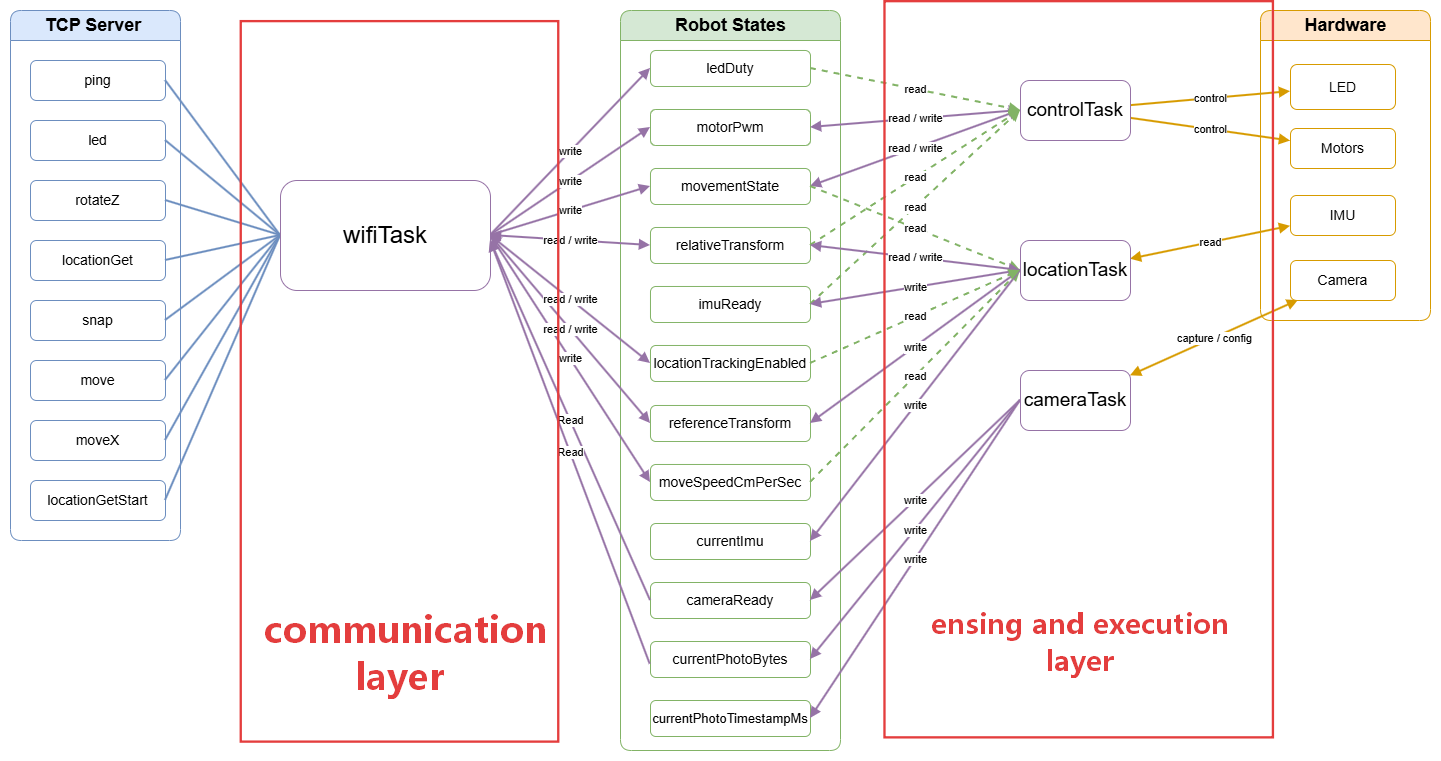
\includegraphics[width=0.92\columnwidth]{figures/robot_code_architecture.drawio.png}
    \caption{RTOS-based robot control architecture centered on the shared \texttt{robot state} object.}
    \label{fig:robot-code-architecture}
\end{figure}
The software maintains a unified global state object, denoted as \texttt{robot state}, which stores the key runtime status of the robot, including the movement mode, motor PWM, actual moving speed, latest captured image, current camera parameters, current IMU output, error logs, reference coordinate frame, and current relative pose. This state object also serves as the interface between the communication layer and the execution layer. As illustrated in Fig.~\ref{fig:robot-code-architecture}, the left side of the architecture can be regarded as the communication layer, while the right side can be regarded as the sensing and execution layer. The communication layer does not directly read or write hardware. Instead, it only reads and modifies the shared \texttt{robot state} object according to the received packets. Conversely, the execution layer does not directly communicate with the communication layer. It continuously updates \texttt{robot state} from hardware observations and maps the relevant state attributes to hardware actions. In this way, the two parts are decoupled through the shared state object rather than directly invoking each other, which helps avoid blocking and makes the program structure clearer.

Among the four tasks, the WiFi feedback task has the highest priority. It is responsible only for communication, as well as reading and modifying the shared state object, but it does not directly perform time-consuming operations such as IMU reading, image acquisition, or pose computation. This task remains suspended during idle periods and is awakened only when a communication packet is received. The robot control task has the second-highest priority and is also suspended most of the time. It is awakened after the WiFi feedback task updates motion-related parameters, and then updates the robot motion according to the movement mode and PWM stored in the shared state~\cite{freertos_ref_manual}.

The photo-reading task and the position-estimation task have the same lower priority and run periodically in the background. The photo-reading task polls the camera at a fixed interval and continuously refreshes the latest image buffer. The position-estimation task reads the IMU periodically and updates the relative pose. By running these two tasks continuously in the background, the system avoids blocking caused by temporary hardware access when a command arrives.

To guarantee consistency in multi-task access to shared data, all shared states are protected by a mutex. In addition, any shared result must be written back to the state object only after the complete computation is finished, rather than through staged partial updates. This ensures that the WiFi feedback task always reads complete and internally consistent data when responding to external requests~\cite{freertos_ref_manual}.

\subsection{Image-to-Point Cloud Reconstruction}
\label{subsec:image-to-point-cloud-method-junjie-ouyang}

\subsubsection{Pipeline Overview}
\label{subsubsec:pipeline-overview-junjie-ouyang}

This submodule converts a single RGB image into a coloured PLY point cloud. The point cloud is then passed to the next stage for point cloud fusion. After that, later stages of the project use the fused result for map generation and path planning. As the first stage of this pipeline, the main aim of the method is to produce a point cloud that is geometrically usable for later processing. An overview of the full processing pipeline is shown in Fig.~\ref{fig:pipeline-junjie}.

\begin{figure}[htbp]
    \centering
    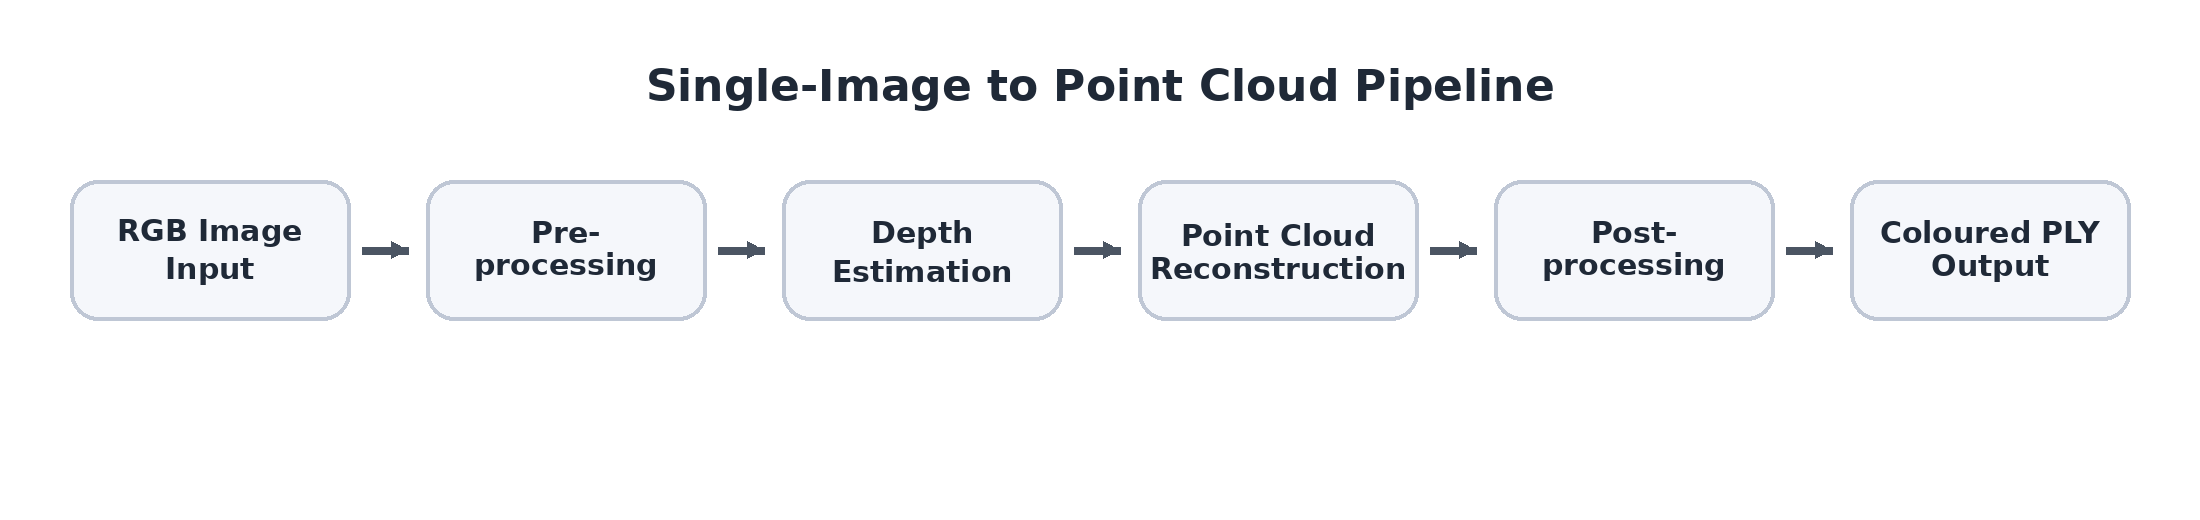
\includegraphics[width=\textwidth]{figures/junjie/pipeline.png}
    \caption{Overview of the single-image point cloud reconstruction pipeline.}
    \label{fig:pipeline-junjie}
\end{figure}

\subsubsection{Image Input and Pre-processing}
\label{subsubsec:image-input-preprocessing-junjie-ouyang}

The input is a single JPG image with a resolution of 1024 $\times$ 768. The system processes one image at a time. A new image is captured and then processed directly. Before depth inference, the image is rotated by 180 degrees. This is done because the camera is mounted upside down during image capture. The output of the submodule is one coloured PLY file for each input image.

\subsubsection{Depth Model Selection}
\label{subsubsec:depth-model-selection-junjie-ouyang}

During early development, a relative-depth model based on Depth Anything V2 was tested~\cite{yang2024}. This model could preserve near--far order in the scene, but it was difficult to use for this project because the depth values could not be linked to real-world distance in a stable mathematical way. For this reason, the final method did not use the relative-depth approach as the main solution.

The final system uses Depth Pro for depth estimation~\cite{bochkovskii2024}. It was selected because its metric depth output was more suitable for practical distance recovery and point cloud reconstruction in this project. After depth prediction, the depth map is converted into a 3D point cloud by back-projection with calibrated camera intrinsics. At a resolution of 1024 $\times$ 768, the calibrated intrinsic parameters were $f_x = 1180.50$, $f_y = 1184.63$, $c_x = 522.11$, and $c_y = 394.13$. In the reconstruction step, $Z$ is treated as the depth value. The $X$ and $Y$ coordinates are computed from pixel position and focal length. Each reconstructed point keeps its RGB colour, and the result is exported as a coloured PLY file.

\subsubsection{Camera Calibration Procedure}
\label{subsubsec:camera-calibration-procedure-junjie-ouyang}

Camera calibration was carried out using a checkerboard-based approach following the general calibration framework proposed by Zhang~\cite{zhang2000}. The intrinsic parameters were estimated from 30 checkerboard images captured from different viewing angles. The final calibration gave an OpenCV RMS value of 0.542 and a mean reprojection error of 0.459 pixels. These results were considered sufficient for the geometric reconstruction stage.

\subsubsection{Point Cloud Post-processing}
\label{subsubsec:point-cloud-postprocessing-junjie-ouyang}

Several post-processing steps are applied after point cloud generation. First, the floor is extended from the nearest visible cross-section back to the origin. This is done to make the near-ground region more complete for the later mapping stage. Second, a virtual square floor patch of 12 cm $\times$ 12 cm is added at the origin. This gives the later path-planning stage a small free region for movement. Third, only the foreground shell is kept. This step uses depth discontinuity to detect strong depth changes and remove the transition band between foreground objects and background structure.

A representative depth map is shown in Fig.~\ref{fig:depth-jump-junjie}. In this example, the front box appears as a clear depth region against the surrounding surface. The shell-preservation step uses the depth jump around the box boundary to identify the foreground region and suppress the transition points near the object edge. This helps reduce trailing scattered points and keeps the object outline clearer for later fusion. The visual effect of this post-processing is shown in Fig.~\ref{fig:before-after-junjie}. Compared with the original output, the processed result contains a cleaner object boundary and fewer trailing points.

\begin{figure}[htbp]
    \centering
    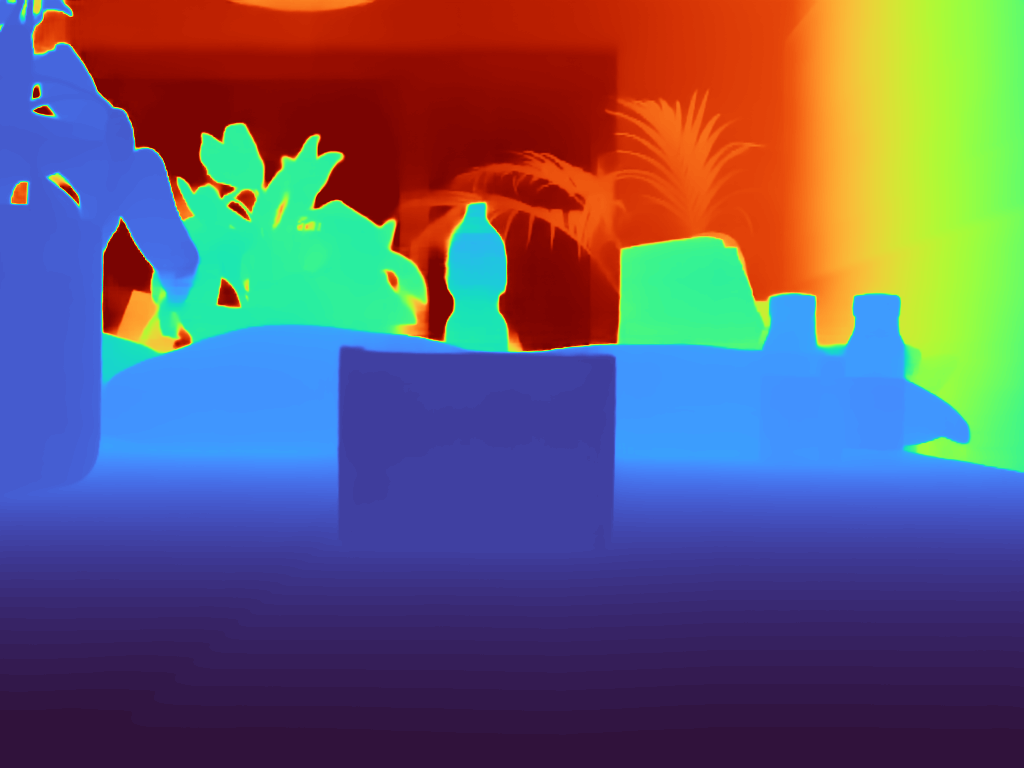
\includegraphics[width=0.68\textwidth]{figures/junjie/depth.png}
    \caption{Depth map used to identify depth discontinuities around the foreground box.}
    \label{fig:depth-jump-junjie}
\end{figure}

\begin{figure}[htbp]
    \centering
    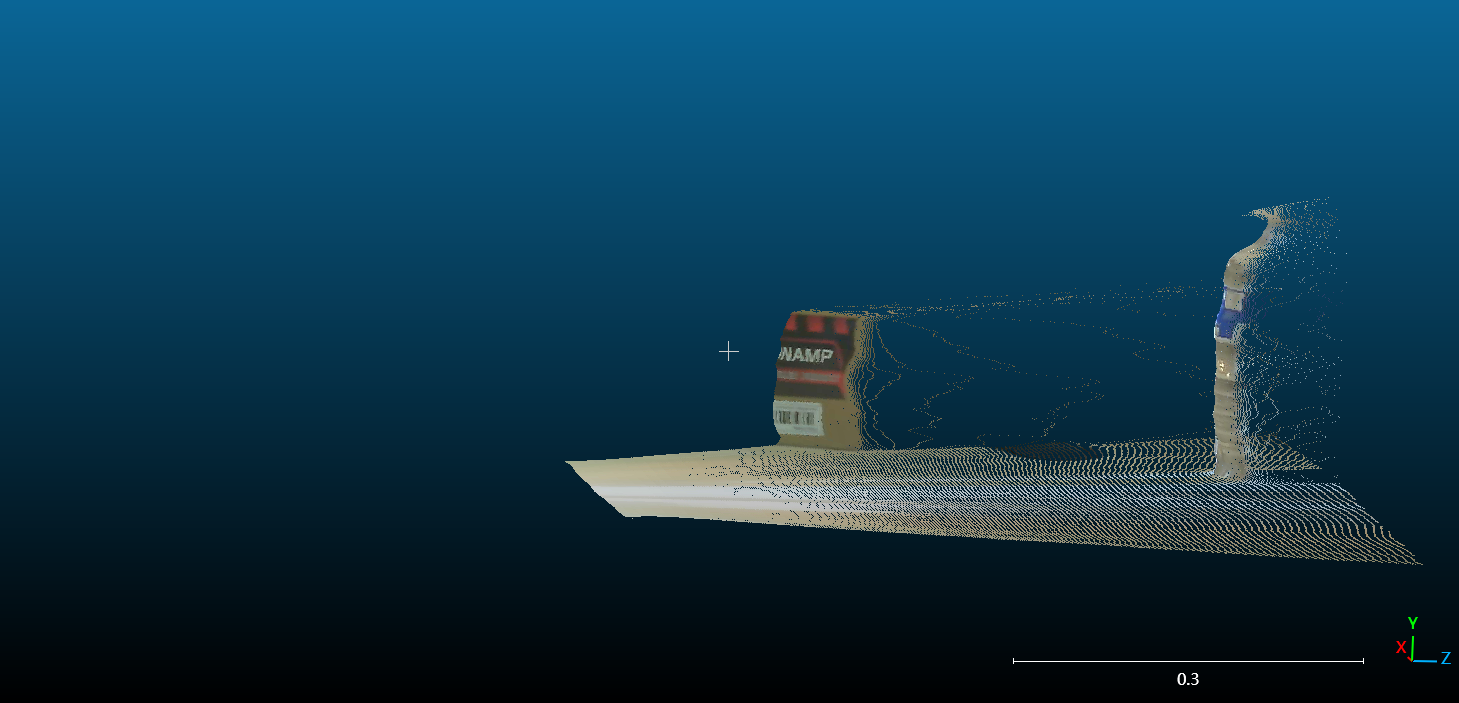
\includegraphics[width=0.9\textwidth]{figures/junjie/before.png}
    \caption*{(a) Before}
    
    \vspace{0.8em}
    
    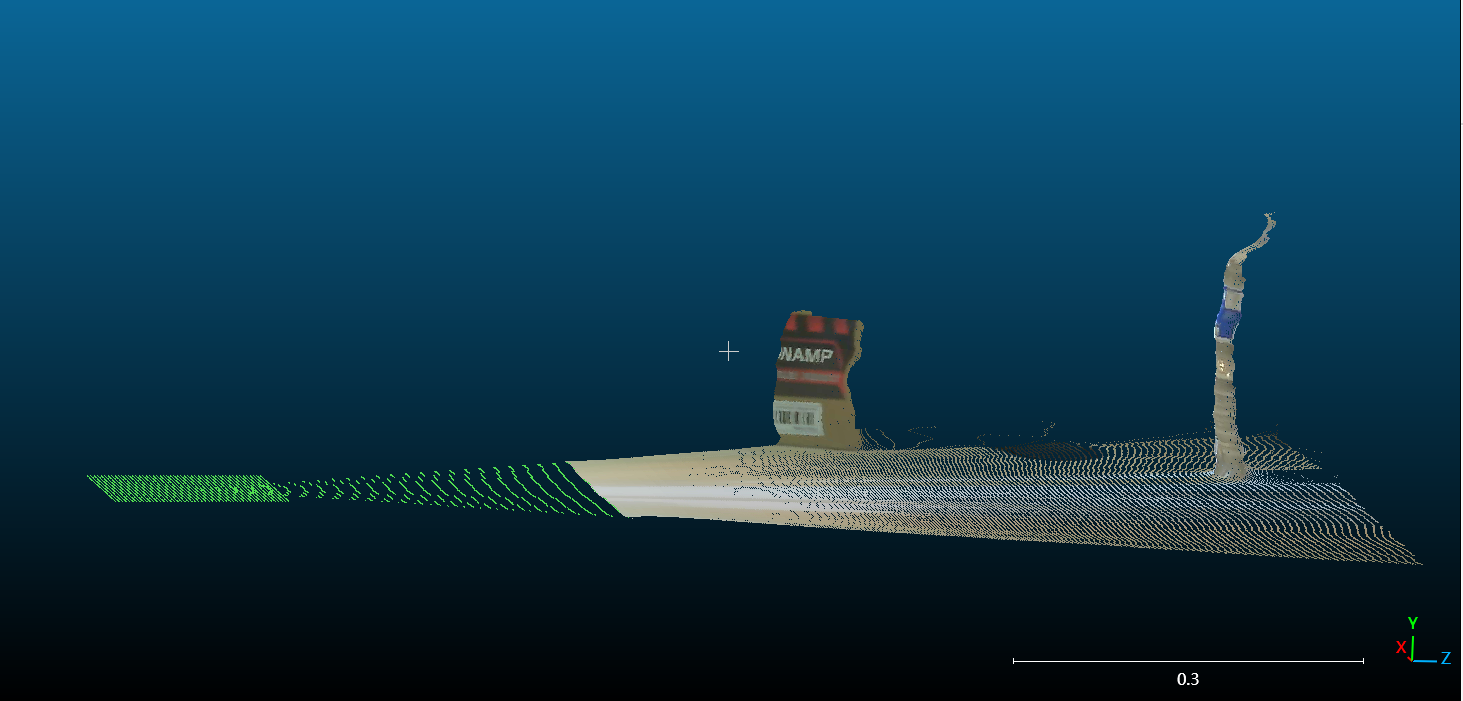
\includegraphics[width=0.9\textwidth]{figures/junjie/after.png}
    \caption*{(b) After}
    
    \caption{Visual comparison before and after post-processing.}
    \label{fig:before-after-junjie}
\end{figure}

\subsubsection{Runtime Performance}
\label{subsubsec:runtime-performance-junjie-ouyang}

The model runs on a GPU. Half-precision inference is enabled to improve speed. Initial model loading takes about 40 seconds. The first image takes about 15 seconds. After that, each later image is processed in about 1.5 seconds. The final setup therefore favours runtime speed, while still keeping point cloud quality at a level that is useful for later stages.

\subsubsection{Distance Accuracy Evaluation}
\label{subsubsec:distance-accuracy-evaluation-junjie-ouyang}

The output is evaluated by comparing measurements taken in CloudCompare with real measurements from the physical scene. The main criteria are distance error, contour clarity, and visible shape distortion. In addition, the point cloud is judged by whether it is suitable for later point cloud fusion.

In this evaluation, all tested distances are based on the same target object, which is the small box placed in front of the camera. The measured distance refers to the distance between the camera and the front surface of the box. Table~\ref{tab:distance-accuracy-junjie} shows the comparison between the real measured distances and the corresponding point cloud measurements for this box at different positions. A visual example of the measurement is shown in Fig.~\ref{fig:accuracy-eval-junjie}.

\begin{table}[htbp]
    \centering
    \caption{Comparison between real measured distances and point cloud measurements for the front surface of the box.}
    \label{tab:distance-accuracy-junjie}
    \begin{tabular}{|c|c|c|}
        \hline
        Real distance (cm) & Point cloud distance (cm) & Absolute error (cm) \\
        \hline
        30  & 34  & 4  \\
        40  & 42  & 2  \\
        50  & 52  & 2  \\
        60  & 61  & 1  \\
        70  & 74  & 4  \\
        80  & 88  & 8  \\
        90  & 100 & 10 \\
        100 & 111 & 11 \\
        \hline
    \end{tabular}
\end{table}

\begin{figure}[htbp]
    \centering
    \begin{subfigure}[t]{0.48\textwidth}
        \vspace{0pt}
        \centering
        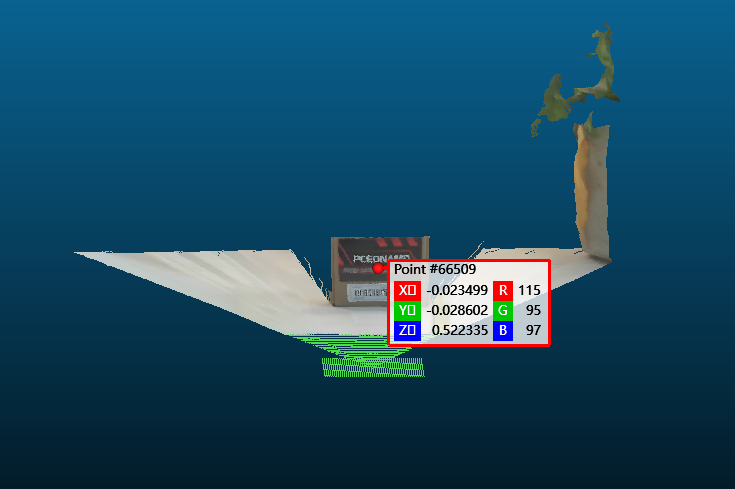
\includegraphics[height=5cm,keepaspectratio]{figures/junjie/point50.png}
        \caption{Point cloud measurement of the box front surface at about 52\,cm.}
        \label{fig:point50-junjie}
    \end{subfigure}
    \hfill
    \begin{subfigure}[t]{0.48\textwidth}
        \vspace{0pt}
        \centering
        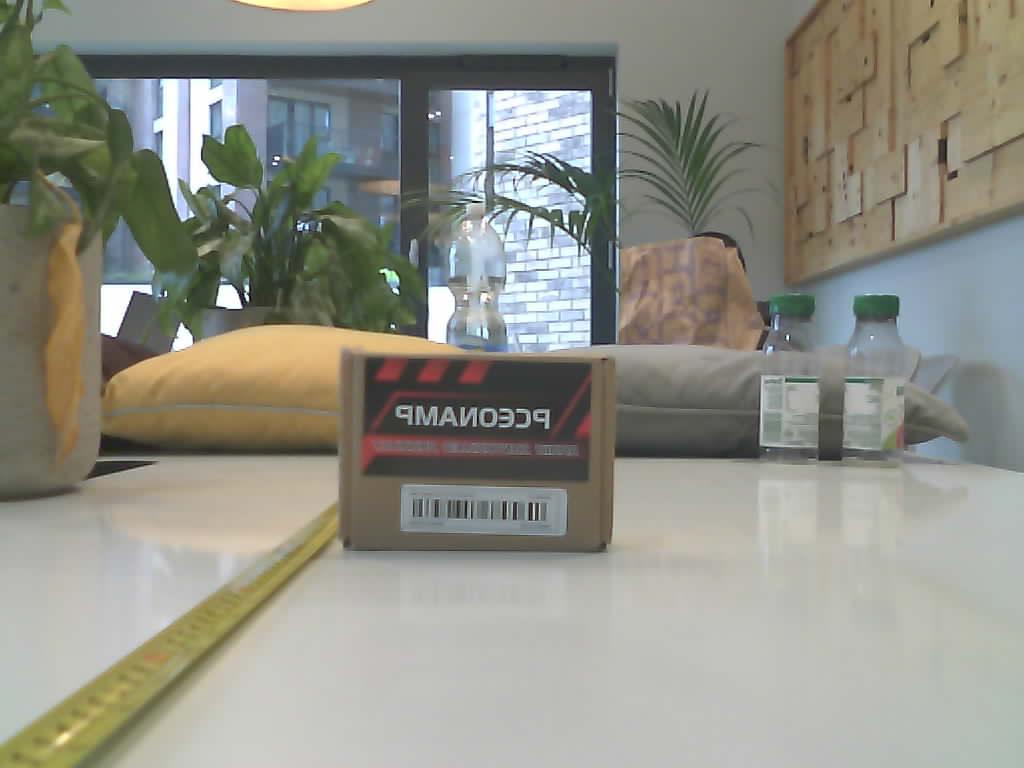
\includegraphics[height=5cm,keepaspectratio]{figures/junjie/real50.png}
        \caption{Real scene measurement of the box front surface at 50\,cm.}
        \label{fig:real50-junjie}
    \end{subfigure}
    \caption{Distance evaluation for the box front surface.}
    \label{fig:accuracy-eval-junjie}
\end{figure}

As shown in Table~\ref{tab:distance-accuracy-junjie}, the point cloud is more accurate at shorter distances. From 30\,cm to 70\,cm, the error stays relatively small. In this range, the absolute error is between 1\,cm and 4\,cm. This means that the reconstructed point positions are still close to the real scene positions. However, the error becomes larger when the distance increases. At 80\,cm, the error rises to 8\,cm. At 90\,cm, it increases to 10\,cm. At 100\,cm, it reaches 11\,cm. This shows a clear overall trend. The farther the box is from the camera, the less accurate the reconstruction becomes.

Another important point is that the point cloud distance is larger than the real distance at every tested position. This means that the reconstruction tends to overestimate distance in this set of measurements. This overestimation is small at short range, but it becomes more obvious at longer range. For example, the difference is only 1\,cm at 60\,cm, but it increases to 11\,cm at 100\,cm. This result suggests that the model output is more reliable in the near field than in the far field.

The 50\,cm case shown in Fig.~\ref{fig:accuracy-eval-junjie} is one of the measurements already included in Table~\ref{tab:distance-accuracy-junjie}. In this case, the real scene distance is 50\,cm, while the point cloud measurement is about 52\,cm. The absolute error is therefore 2\,cm. This matches the overall trend in the table and gives a direct visual example of the evaluation method.

Based on these results, the final point cloud is limited to a working range of 1\,m from the camera. The reason is that the error becomes too large at longer distance. By restricting the effective range, the system can keep better geometric accuracy for later point cloud fusion. A better result is therefore one that gives smaller distance error, clearer object boundaries, and less unwanted deformation within this effective range.


\subsection{Point Cloud Merging}
\label{subsec:system-overview-mapper-pipeline-qingzhou-zhang}
\subsubsection{System Overview and Mapper Pipeline}

The point cloud merging system is developed in a modular manner. Each internal functionality is divided into independent submodules and invoked through concise interfaces. This design improves the extensibility and maintainability of the system, allowing modules to be replaced or extended without affecting the overall structure. At the same time, low coupling between modules is maintained to avoid cascading effects caused by local modifications.

In the overall architecture, the Mapper acts as the core scheduling unit. It does not implement functions but is responsible for organizing and connecting modules to construct a complete processing pipeline.

\begin{figure}[!htbp]
    \centering
    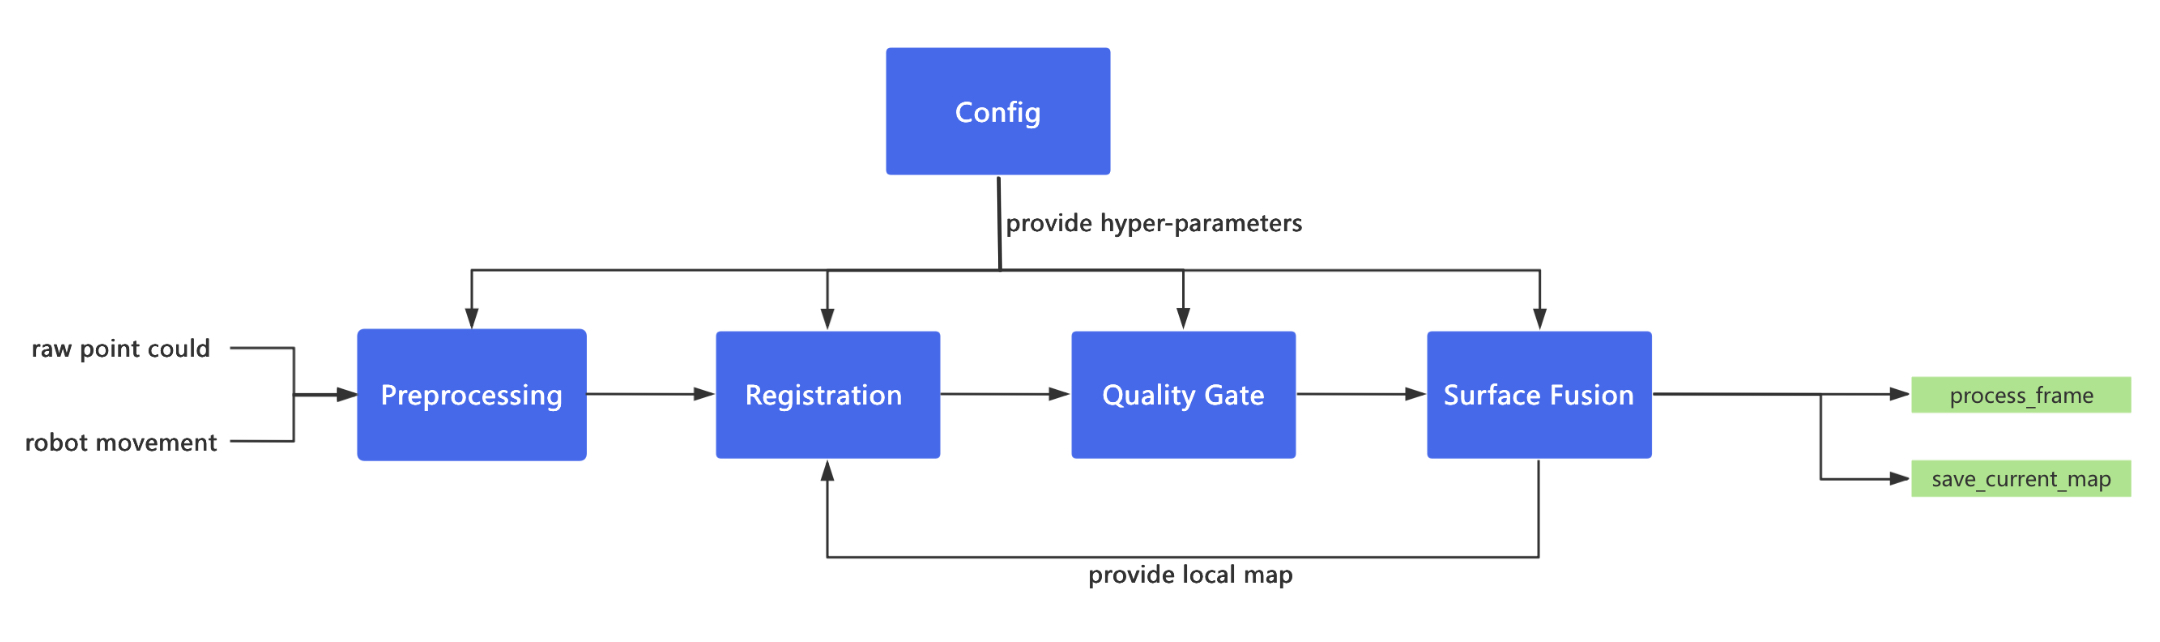
\includegraphics[width=\linewidth]{figures/qingzhou/mapper schematic.jpg}
    \caption{Mapper pipeline schematic.}
    \label{fig:mapper-pipeline-schematic-qingzhou}
\end{figure}

The Mapper provides two main external interfaces: \texttt{process\_frame} and \texttt{save\_current\_map}. Among them, \texttt{process\_frame} is the core interface used to process single-frame input data. This method receives pose estimation and raw point cloud data from upstream modules, and sequentially performs point cloud preprocessing, registration, and surface fusion according to the predefined pipeline, ultimately outputting the optimized pose of the current frame and the updated local map result. The entire process forms an incremental processing mechanism based on single-frame input, enabling the system to construct the global map frame by frame.

The \texttt{save\_current\_map} interface is used to export the currently constructed global map and is typically invoked after data acquisition or processing is completed. Separating real-time processing from result exporting helps ensure that only single-frame data is handled in the main loop, thereby avoiding additional data transfer and computational overhead as the map size grows.

In addition, the system provides a \texttt{report} interface for recording and exporting runtime statistical information. This interface collects key metrics after each frame is processed and finally generates a text report file, providing data support for debugging, performance analysis, and result evaluation.

\subsubsection{Registration and Supporting Modules}

This module refines the pose of the current frame from an externally provided prior transformation through local registration, while incorporating a result gating mechanism to prevent unreliable alignment results from propagating into the map. As shown in Fig.~\ref{fig:registration-schematic-qingzhou}, the registration pipeline consists of five stages: prior pose construction, point cloud preprocessing, local map extraction, registration, and result validation.

\begin{figure}[htbp]
    \centering
    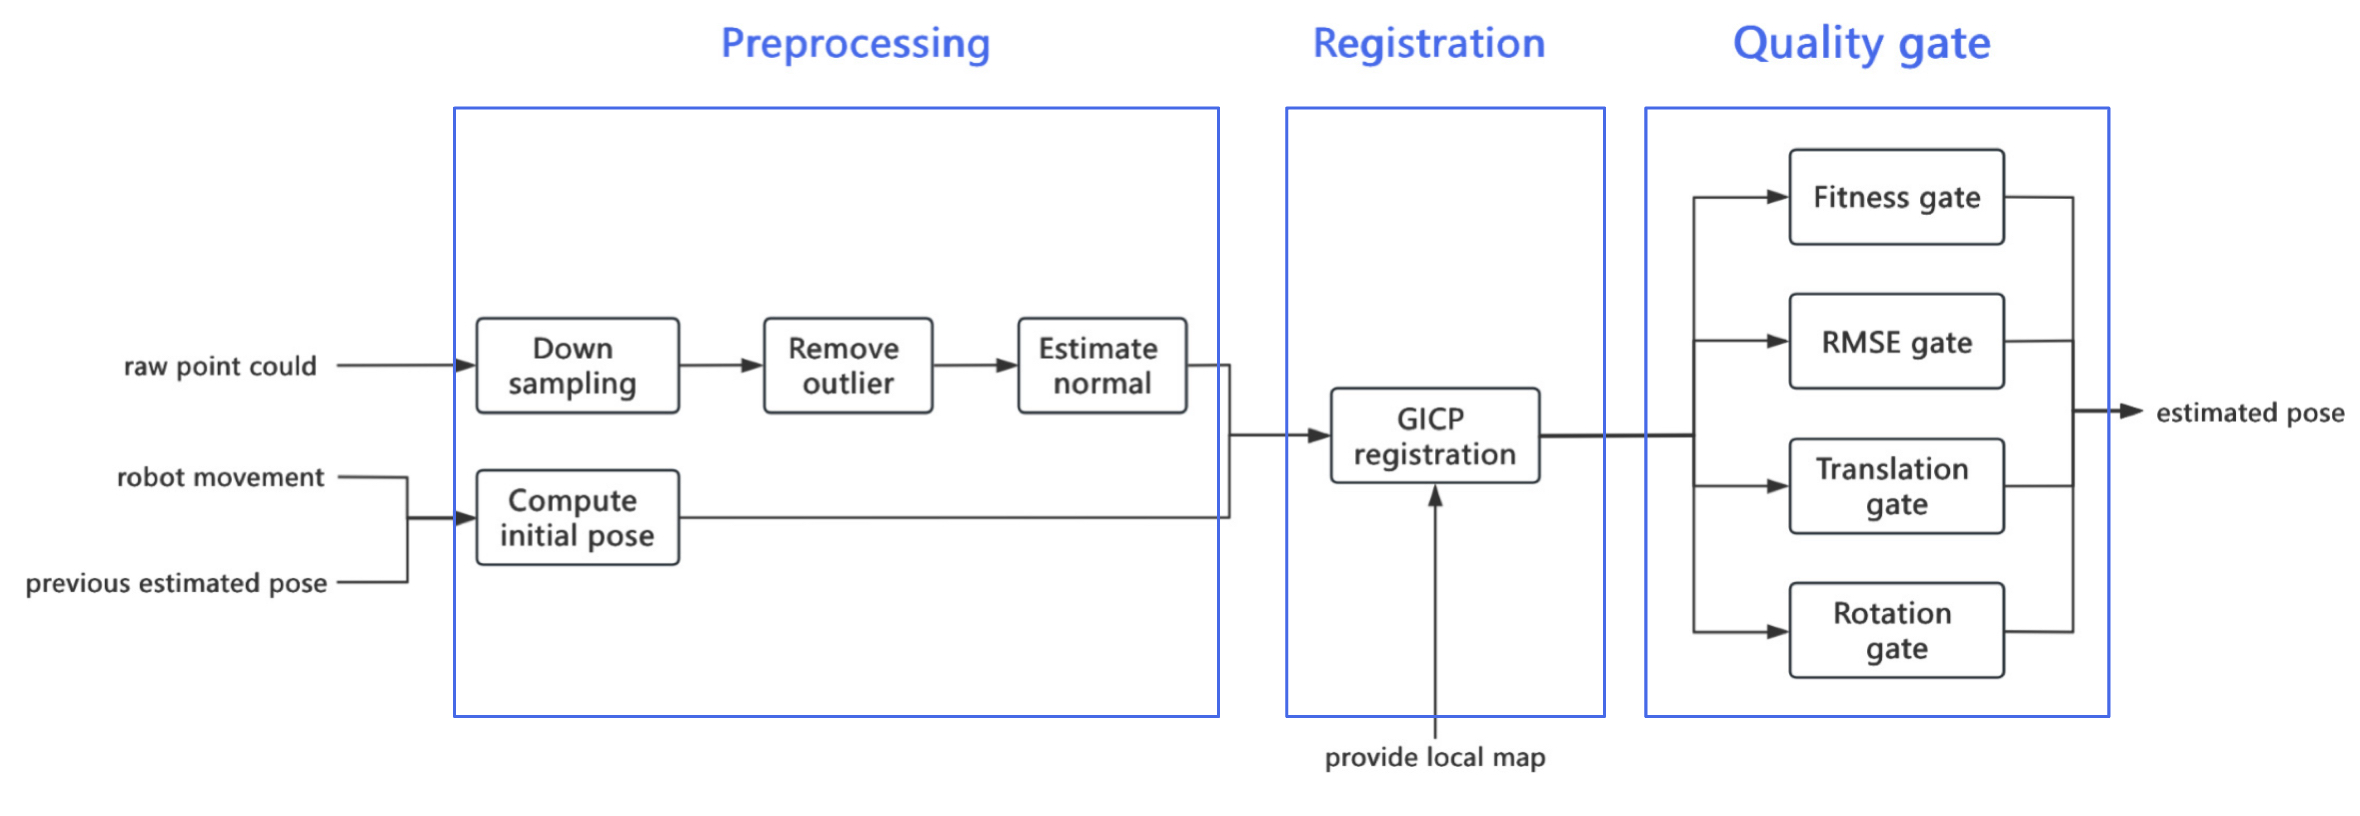
\includegraphics[width=\linewidth]{figures/qingzhou/registraion schematic.jpg}
    \caption{Registration schematic.}
    \label{fig:registration-schematic-qingzhou}
\end{figure}

First, an initial pose is constructed for the current frame. For ordinary frames, this prior is obtained by composing the global pose of the previous frame with the externally estimated inter-frame motion increment. For the first frame, the input pose is used directly. This prior serves as the starting point for the subsequent local registration.

Next, the input point cloud is preprocessed before alignment. This stage includes voxel downsampling, statistical outlier removal, and normal estimation. The purpose of preprocessing is to reduce the computational burden of registration, suppress unstable observations, and provide reliable local geometric information for the subsequent GICP optimization. The specific parameter settings used in this module are summarized in Table~\ref{tab:registration-params-qingzhou}.

After preprocessing, a local submap is extracted from the current surfel map around the translational component of the initial pose. Restricting the target point set to a local neighborhood avoids the high computational cost and mismatch risk associated with global-scale registration, while remaining sufficient for local pose refinement.

The registration stage is initialized from the prior pose and solved using GICP, which iteratively estimates the relative rigid transformation between the current frame and the extracted local submap. In this design, the external prior provides the coarse alignment, while GICP performs local geometric refinement around that prior. A coarse registration method based on FPFH and RANSAC with color assistance is also retained in the codebase; however, due to unsatisfactory performance, it is not enabled in the final system, as discussed in Appendix~\ref{subsec:feature-coarse-registration-qingzhou-zhang}.

After the GICP optimization, the estimated result is checked by a quality gate. The validation considers both geometric consistency and deviation from the prior pose. If the alignment quality is insufficient, or if the estimated correction is excessively large relative to the initial pose, the registration result is rejected and the system falls back to the prior transformation. This mechanism suppresses the accumulation of local registration failures and improves the robustness of subsequent map fusion.

Finally, the validated pose is used to transform the current frame point cloud into the map coordinate system and pass it to the surfel-based fusion module. In parallel, the Report module records the final pose and gating outcome for later analysis and debugging.

\begin{table}[htbp]
\centering
\caption{Key hyperparameters of the registration module.}
\label{tab:registration-params-qingzhou}
\begin{tabular}{p{3.2cm}p{1.8cm}p{7.2cm}}
\hline
\textbf{Parameter} & \textbf{Value} & \textbf{Purpose} \\
\hline
Voxel size & 0.01 m & Preprocessing: downsample points while preserving local geometry \\
Outlier neighbors & 20 & Preprocessing: define the local neighborhood for statistical filtering \\
Outlier std. ratio & 5.0 & Preprocessing: reject points with large local deviation \\
Normal estimation radius & 0.03 m & Preprocessing: estimate stable local surface normals \\
Normal max neighbors & 30 & Preprocessing: limit neighborhood size in normal estimation \\
Local map radius & 3.0 m & Local map extraction: restrict registration to a nearby submap \\
Max correspondence distance & 0.10 m & GICP: suppress distant and likely incorrect matches \\
Max GICP iterations & 100 & GICP: limit iterative optimization cost \\
Minimum fitness & 0.40 & Quality gate: reject weak geometric alignment \\
Maximum RMSE & 0.08 m & Quality gate: constrain registration residual error \\
Max translation correction & 0.25 m & Quality gate: limit deviation from the prior pose \\
Max rotation correction & $15^\circ$ & Quality gate: limit excessive rotational correction \\
\hline
\end{tabular}
\end{table}

\begin{figure}[htbp]
    \centering
    \begin{subfigure}[b]{0.49\linewidth}
        \centering
        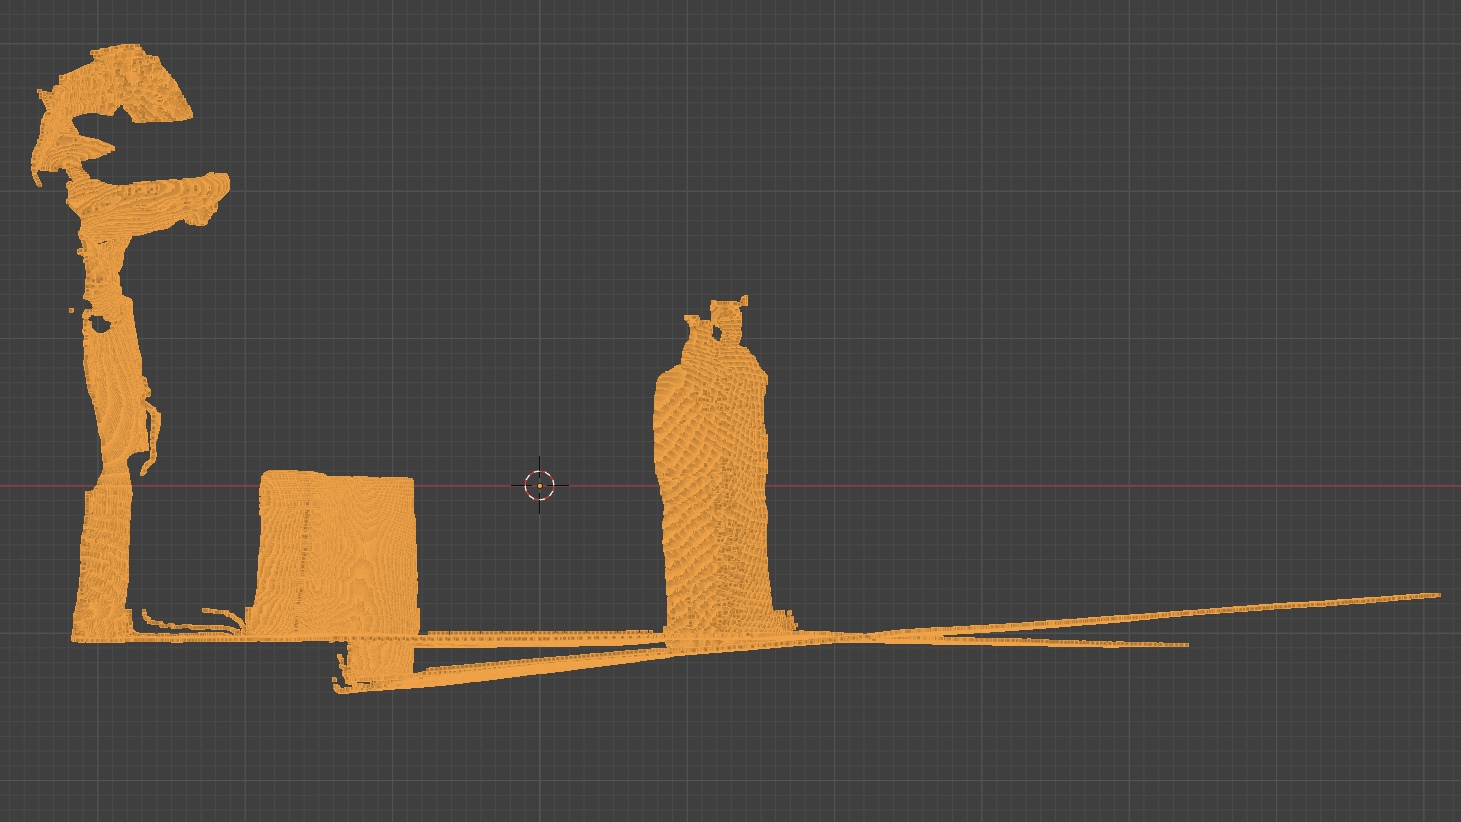
\includegraphics[width=\textwidth]{figures/qingzhou/before_registration_2.jpg}
        \caption{Without GICP registration.}
    \end{subfigure}
    \hfill
    \begin{subfigure}[b]{0.49\linewidth}
        \centering
        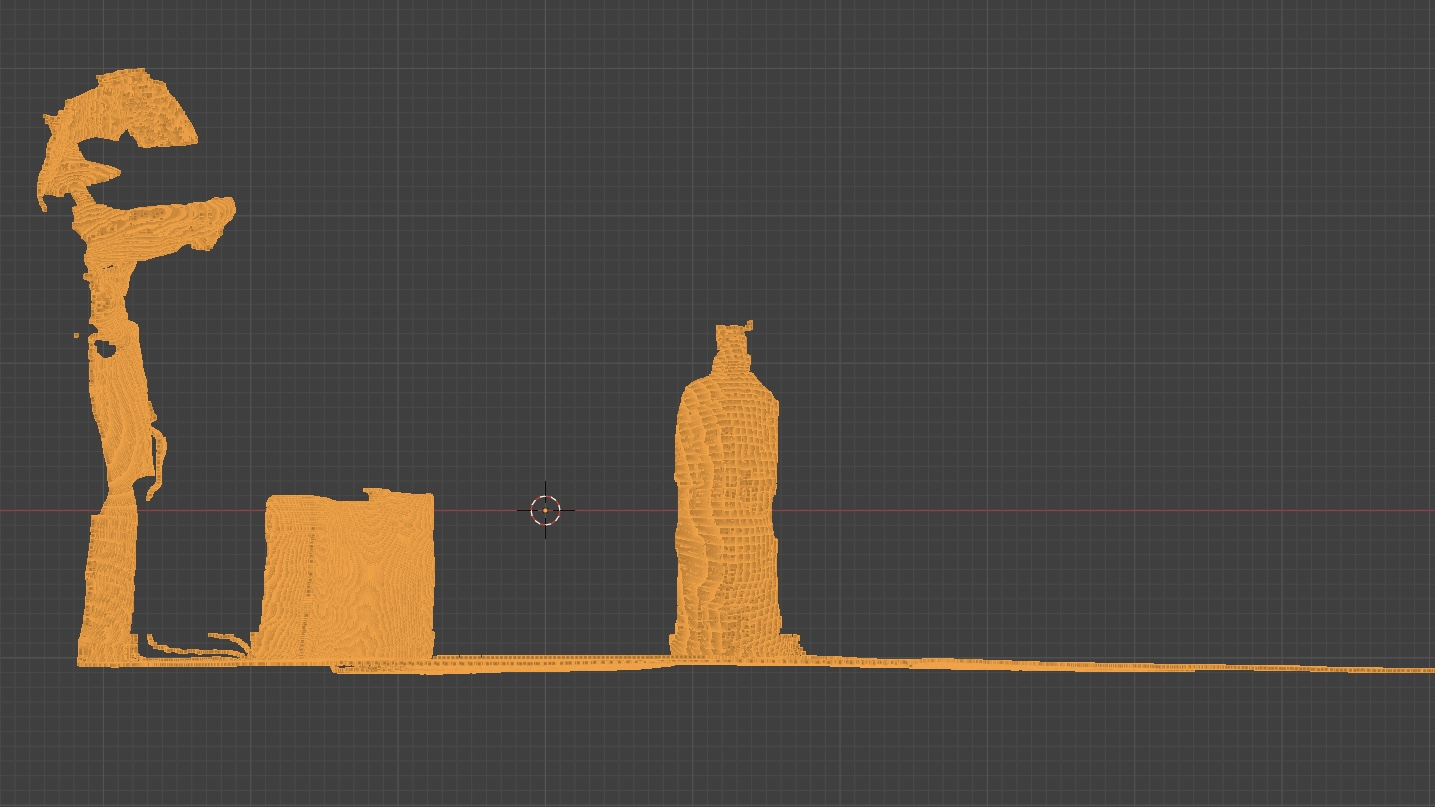
\includegraphics[width=\textwidth]{figures/qingzhou/after_registration.jpg}
        \caption{With GICP registration.}
    \end{subfigure}
    \caption{Comparison of registration performance.}
    \label{fig:comparison-registration-qingzhou}
\end{figure}

\subsubsection{Surface Fusion Module}

After registration is completed for the current frame, the surface fusion module incrementally integrates observation points into the global map and continuously updates and maintains it. This module uses surfels as the basic surface representation unit, including geometric attributes, appearance attributes, and observation statistical attributes. The geometric attributes include position and normal, the appearance attributes include color description, and the statistical attributes include accumulated weight, creation frame, last observed frame, and observation count.

Overall, the program adopts a voxel-based spatial organization to manage the global map. Each voxel maintains a limited number of surfels, balancing local query efficiency and map size control.

During each frame fusion process, the program first constructs an active region based on the current observation area and searches for candidate surfels only within this local region. For each observation point, nearby surfels are searched within a given radius and filtered based on spatial distance, normal consistency, and color similarity. Only when both geometric and appearance constraints are satisfied are the observation and surfel considered associable. If multiple valid candidates exist, the best match is selected based on combined differences. This strategy aims to reduce computational complexity and the risk of incorrect fusion.

For observation points successfully associated with surfels, the program adopts a consistency-based weighted update strategy to fuse surfel attributes. Let the current observation point be $p$, the corresponding surfel position be $s$, the accumulated weight be $w$, and the current observation weight be $w_{\text{obs}}$. The weight $w_{\text{obs}}$ is jointly determined by the distance, normal difference, and color difference between the observation and the surfel, with higher consistency leading to larger weights.

The updated total weight is:

\begin{equation}
w_{\text{new}} = w + w_{\text{obs}}
\end{equation}

The position is updated using weighted averaging:

\begin{equation}
s_{\text{new}} = \frac{w s + w_{\text{obs}} p}{w_{\text{new}}}
\end{equation}

Normal and color attributes are updated in the same manner, with normals re-normalized after updating. This mechanism allows stable historical observations to continuously provide prior constraints, while new observations that are more consistent with the surfel exert stronger influence, leading to progressively smoother and more stable surface estimation.

For observation points that cannot be matched to any suitable surfel, the program creates new surfels at the corresponding spatial locations to complement regions not yet sufficiently represented in the map. The initial attributes of new surfels are directly assigned from the current observation and are gradually refined through subsequent multi-frame fusion. In this way, the map can adaptively expand as more observations are incorporated.

To maintain compactness and long-term stability of the map, the program introduces maintenance mechanisms including intra-voxel merging, capacity pruning, and periodic cleaning. For surfels that are spatially close and similar in attributes, merging is performed within voxels to reduce redundancy and improve local consistency. When the number of surfels in a voxel exceeds a predefined limit, surfels with higher observation confidence, greater weights, and more stable states are preferentially retained. Additionally, surfels that have not been updated for a long time or have low weights and insufficient observations are periodically removed to suppress noise and outdated information.
\begin{figure}[htbp]
    \centering
    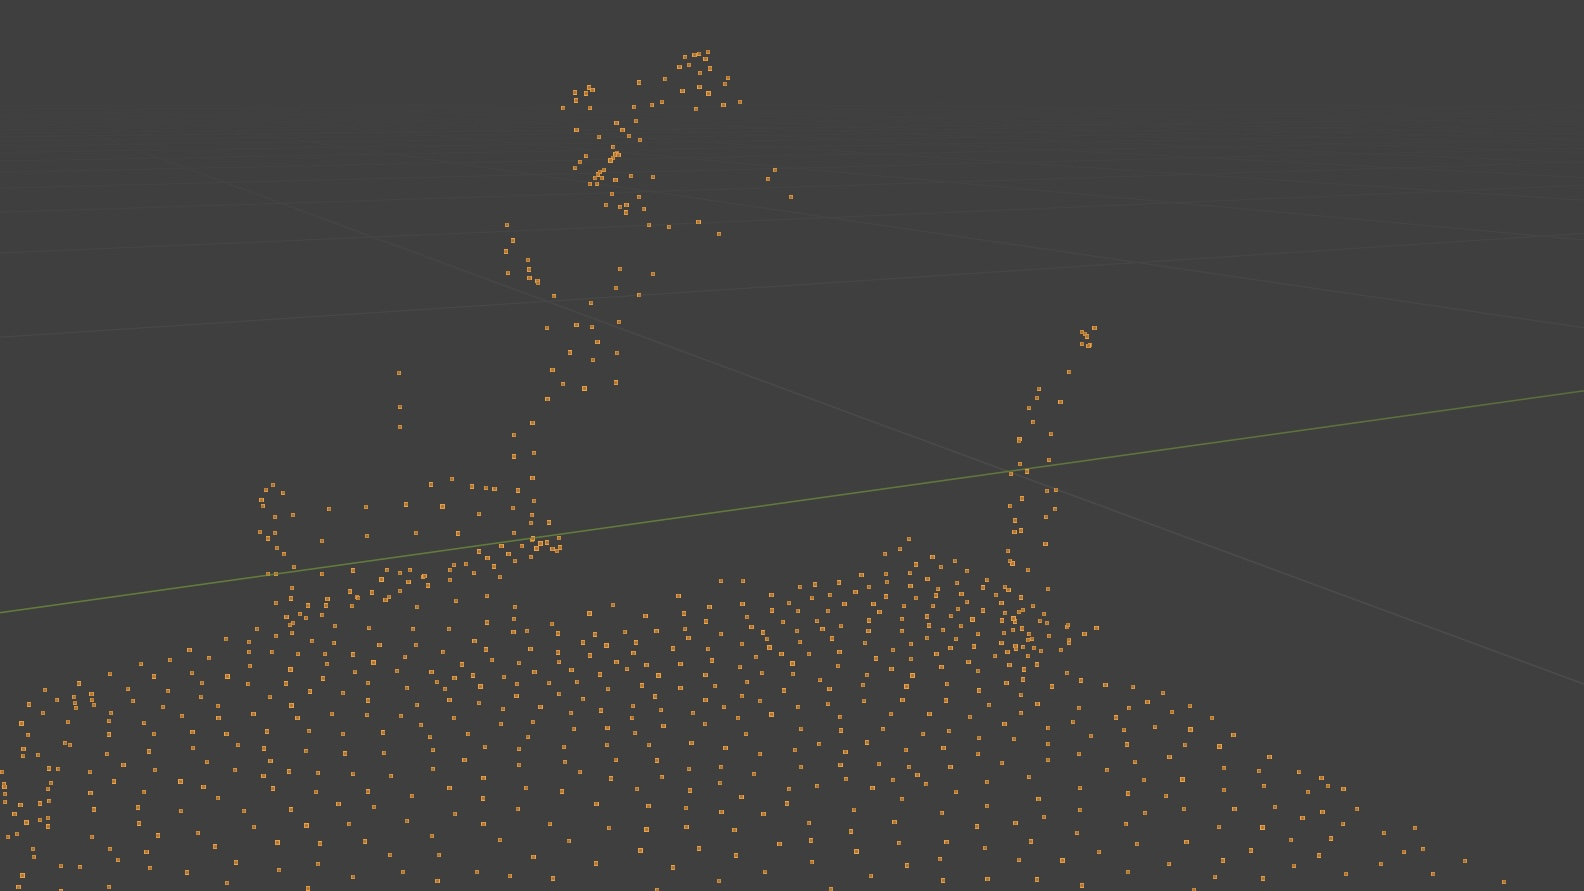
\includegraphics[width=\linewidth]{figures/qingzhou/after fusion.jpg}
    \caption{Merged result with surface fusion.}
    \label{fig:after-surface-fusion-qingzhou}
\end{figure}



\subsection{2D Map Generation and Cost Modeling}
\label{subsec:2dmap-generation-cost-modeling-zhuyu-dong}

To convert the fused 3D point cloud into a representation suitable for path planning, the environment is discretized into regular 2D grid cells~\cite{elfes1989occupancy,gu2008traversability}. Each cell can only be assigned one of three states: \texttt{block}, \texttt{costing}, or \texttt{unknown}. Here, \texttt{block} means that the region is not traversable, \texttt{costing} means that the region is traversable but associated with a traversal cost, and \texttt{unknown} means that the region has not yet been scanned or has not been reliably observed. The robot is allowed to move only through cells labeled as \texttt{costing}. For \texttt{costing} cells, the traversal cost ranges from 0 to 255, where a larger value indicates worse road condition and greater traversal difficulty. If the final cost of a cell is greater than or equal to 255, the cell is also treated as \texttt{block}.

Each grid cell is defined as \(5\text{ cm} \times 5\text{ cm}\). This resolution is selected according to the robot size and a safety margin. The robot body is approximately \(10 \times 10 \times 11\text{ cm}\), and the diameter of its self-rotation coverage is about
\[
2\sqrt{5^2+5^2}\approx 14\text{ cm}.
\]
To reserve additional redundancy, the robot is approximated as a \(15 \times 15 \times 15\text{ cm}\) cube. Under this setting, the \(5\text{ cm} \times 5\text{ cm}\) grid provides a convenient resolution for local traversability evaluation. If the neighboring cells covered by the projected robot footprint are all labeled as \texttt{costing}, the region can be considered traversable.

\subsubsection{Costing computation.}
The 2D map is generated by first performing ground-layer selection on the point cloud~\cite{meng2018terrain}. After the ground layer is determined for each cell, the system checks whether an obstacle exists within a height threshold \(H_{th}\) above the ground layer. If such an obstacle is detected, the cell is directly labeled as \texttt{block}. In this work, the height threshold is set to
\[
H_{th}=15\text{ cm},
\]
which is slightly larger than the robot height of about \(11\text{ cm}\) in order to provide a safety margin.

If no obstacle is found within the threshold, the cell enters the \texttt{costing} stage. The traversal cost is computed from both slope and local complexity~\cite{gu2008traversability,meng2018terrain}. The slope is estimated from the local eigenvector~\cite{weinmann2013feature}. Since the robot can reliably climb slopes up to about \(30^\circ\), the interval from \(0^\circ\) to \(30^\circ\) is linearly mapped to a cost range of 0 to 255. If the slope exceeds \(30^\circ\), the corresponding cell is directly labeled as \texttt{block}.

In addition, the local complexity is computed from the normalized eigenvalue-based roughness measure~\cite{weinmann2013feature}. A larger normalized value indicates a more irregular surface. When the three eigenvalues are equal, the local point set can be regarded as being uniformly distributed in a \(5\text{ cm} \times 5\text{ cm} \times 5\text{ cm}\) volume, which corresponds to the maximum complexity. Its normalized value is approximately
\[
\sqrt{\frac{1}{3}} \approx 0.6.
\]
When the complexity is one tenth of this maximum value, the normalized result becomes
\[
\sqrt{\frac{1}{30}} \approx 0.18.
\]
Therefore, the complexity threshold is set to 0.18. This threshold is chosen because the robot can stably pass obstacles of about \(0.5\text{ cm}\) without significantly affecting pose estimation, so one tenth of the maximum complexity is taken as a practical tolerance level.

The relationship between complexity and actual obstacle severity is not linear, but closer to a quadratic trend. Therefore, the complexity cost is defined as
\[
cost(c)=255\left(\frac{c}{0.18}\right)^2,
\]
where \(c\) is the local complexity value.

\subsubsection{Environment types and state conversion.}
\begin{figure}[htbp]
\centering
\begin{subfigure}[b]{0.64\columnwidth}
    \centering
    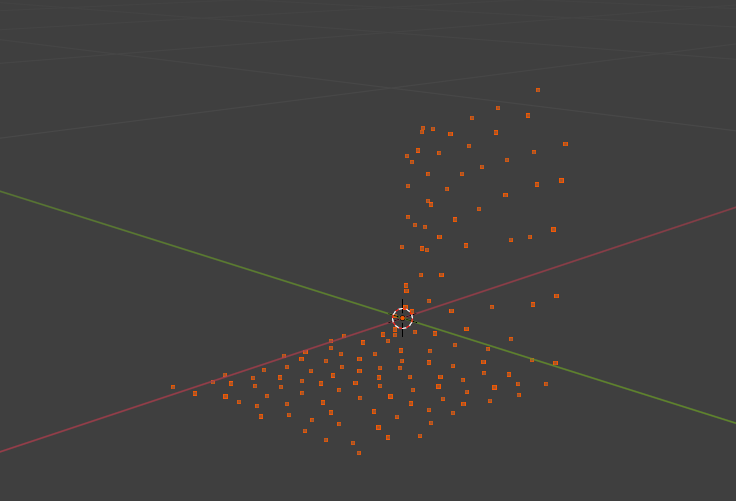
\includegraphics[width=\columnwidth]{figures/2DMAP/WALL.png}
    \caption{Wall or step obstacle.}
    \label{fig:2dmap-wall}
\end{subfigure}
\hfill
\begin{subfigure}[b]{0.315\columnwidth}
    \centering
    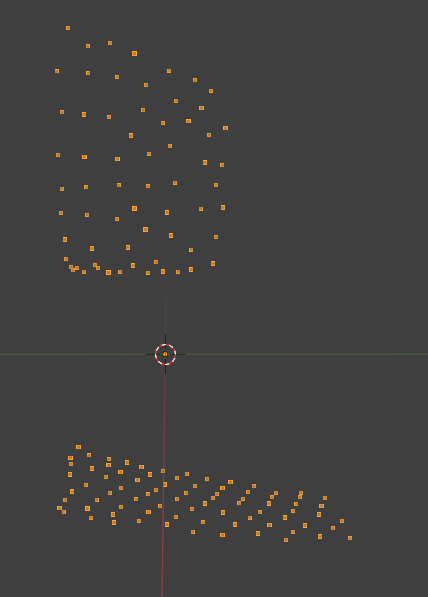
\includegraphics[width=\columnwidth]{figures/2DMAP/Suspended BLOCK.png}
    \caption{Suspended obstacle.}
    \label{fig:2dmap-suspended}
\end{subfigure}
\hfill
\begin{subfigure}[b]{0.47\columnwidth}
    \centering
    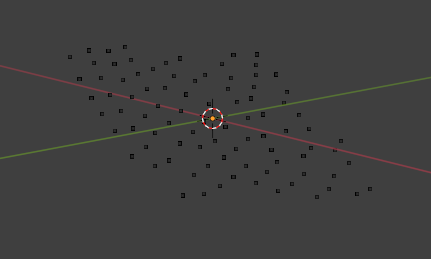
\includegraphics[width=\columnwidth]{figures/2DMAP/SLOPE.png}
    \caption{Slope or traversable uneven region.}
    \label{fig:2dmap-slope}
\end{subfigure}
\hfill
\begin{subfigure}[b]{0.47\columnwidth}
    \centering
    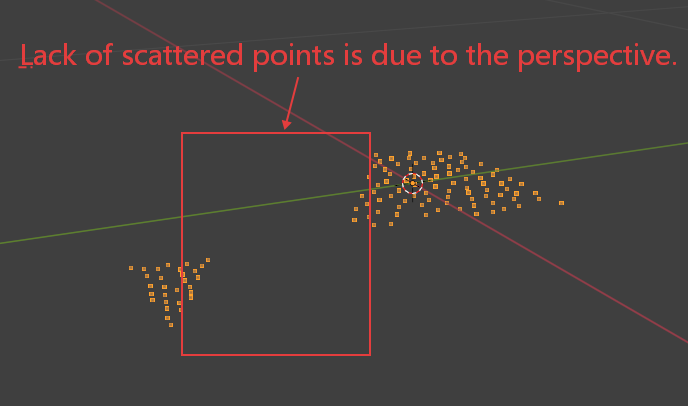
\includegraphics[width=\columnwidth]{figures/2DMAP/PIT.png}
    \caption{Pit or cliff-like region.}
    \label{fig:2dmap-pit}
\end{subfigure}
\caption{Typical obstacle and terrain types considered in the 2D map generation process.}
\label{fig:2dmap-obstacles}
\end{figure}
Four typical environment types are considered in this work: walls or steps, suspended obstacles, planar or sloped regions, and pits or cliff-like regions.

Walls, steps, and suspended obstacles are handled in a similar manner. After ground-layer selection, these structures usually appear as elevated obstacles within a limited height range above the detected ground layer. Therefore, once such an obstacle is found within \(H_{th}\), the corresponding cell is directly classified as \texttt{block}. Planar regions and slopes are mainly represented through slope and complexity, and are therefore converted into different \texttt{costing} values. Small local obstacles are also reflected by increased local complexity, which raises the traversal cost of the corresponding cells~\cite{gu2008traversability,meng2018terrain}.

Pits and cliffs exhibit a different behavior. Due to viewpoint limitations, these regions are often difficult to observe completely during early scanning stages, and their edges or walls may not be reconstructed reliably. As a result, such regions are usually labeled as \texttt{unknown} first, which prevents the robot from entering potentially dangerous areas. After more observations are collected, these regions may later be reclassified as \texttt{costing} or \texttt{block}. Typical examples of these environment types are shown in Fig.~\ref{fig:2dmap-obstacles}.



\subsubsection{Map overwrite and merging.}
\begin{figure}[h] 
\centering
\begin{subfigure}[b]{0.21\columnwidth}
    \centering
    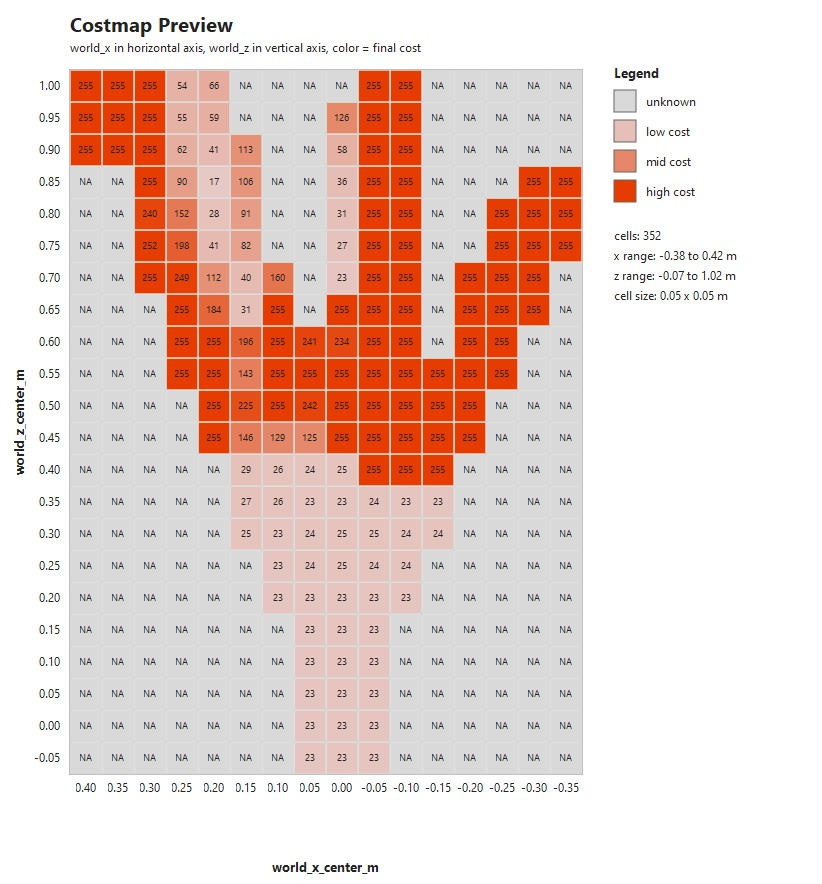
\includegraphics[width=\columnwidth]{figures/merge2dmap/2/map_costmap_view.jpg}
    \caption{Step 1}
    \label{fig:merge2dmap-step1}
\end{subfigure}
\hfill
\begin{subfigure}[b]{0.22\columnwidth}
    \centering
    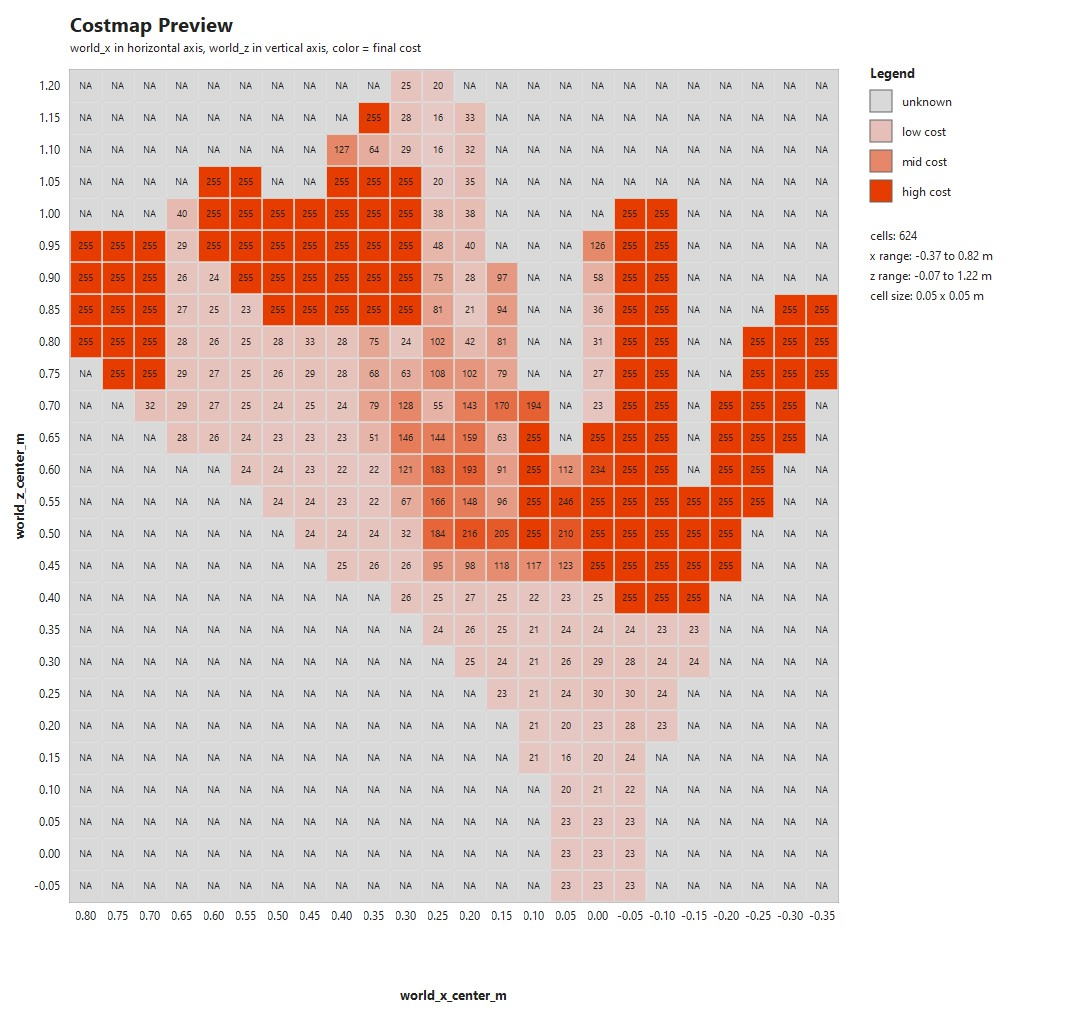
\includegraphics[width=\columnwidth]{figures/merge2dmap/3/map_costmap_view.jpg}
    \caption{Step 2}
    \label{fig:merge2dmap-step2}
\end{subfigure}
\hfill
\begin{subfigure}[b]{0.23\columnwidth}
    \centering
    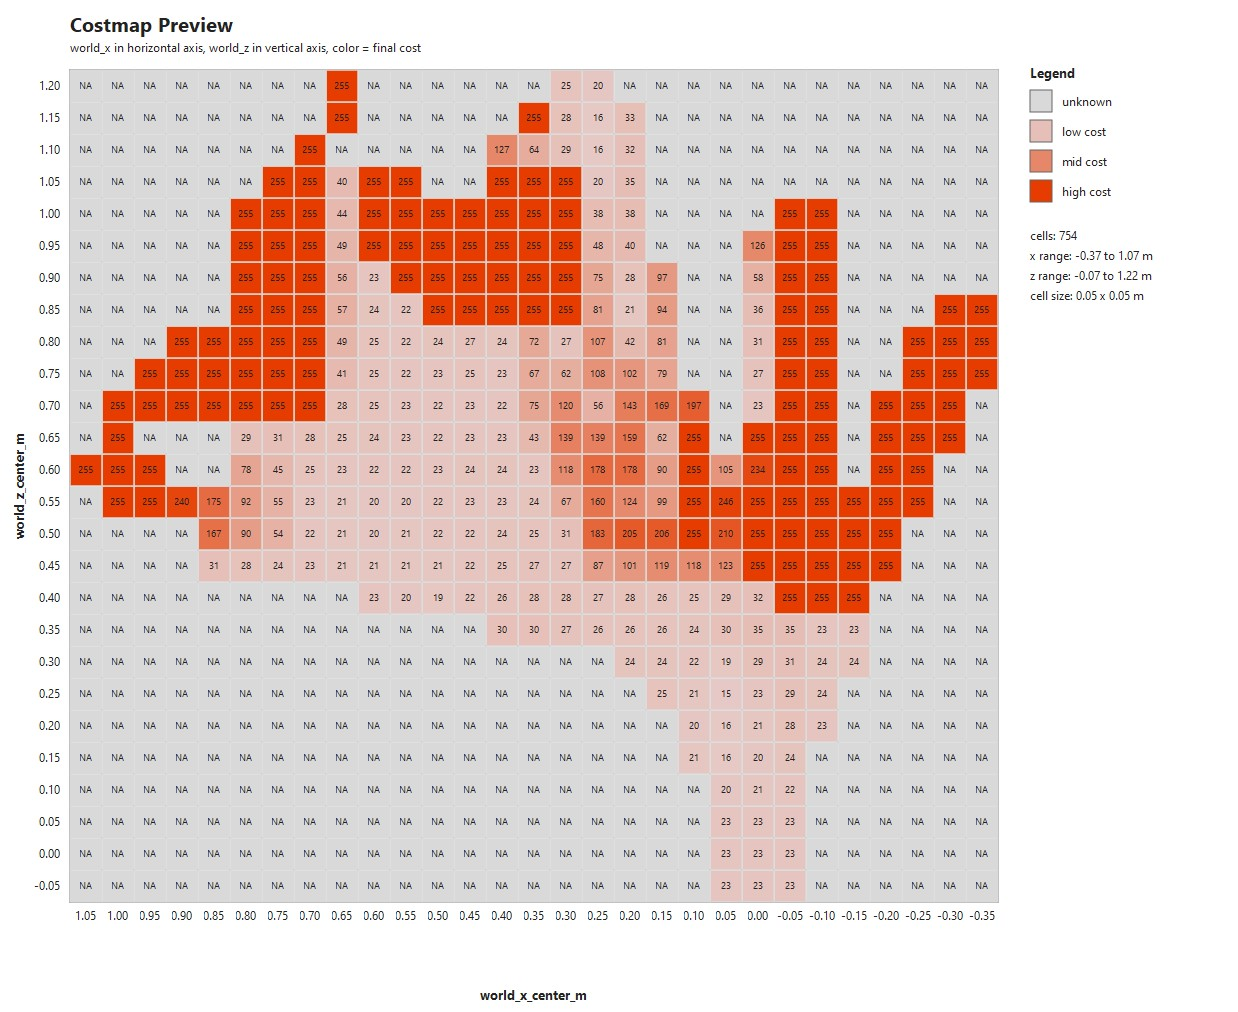
\includegraphics[width=\columnwidth]{figures/merge2dmap/4/map_costmap_view.jpg}
    \caption{Step 3}
    \label{fig:merge2dmap-step3}
\end{subfigure}
\hfill
\begin{subfigure}[b]{0.23\columnwidth}
    \centering
    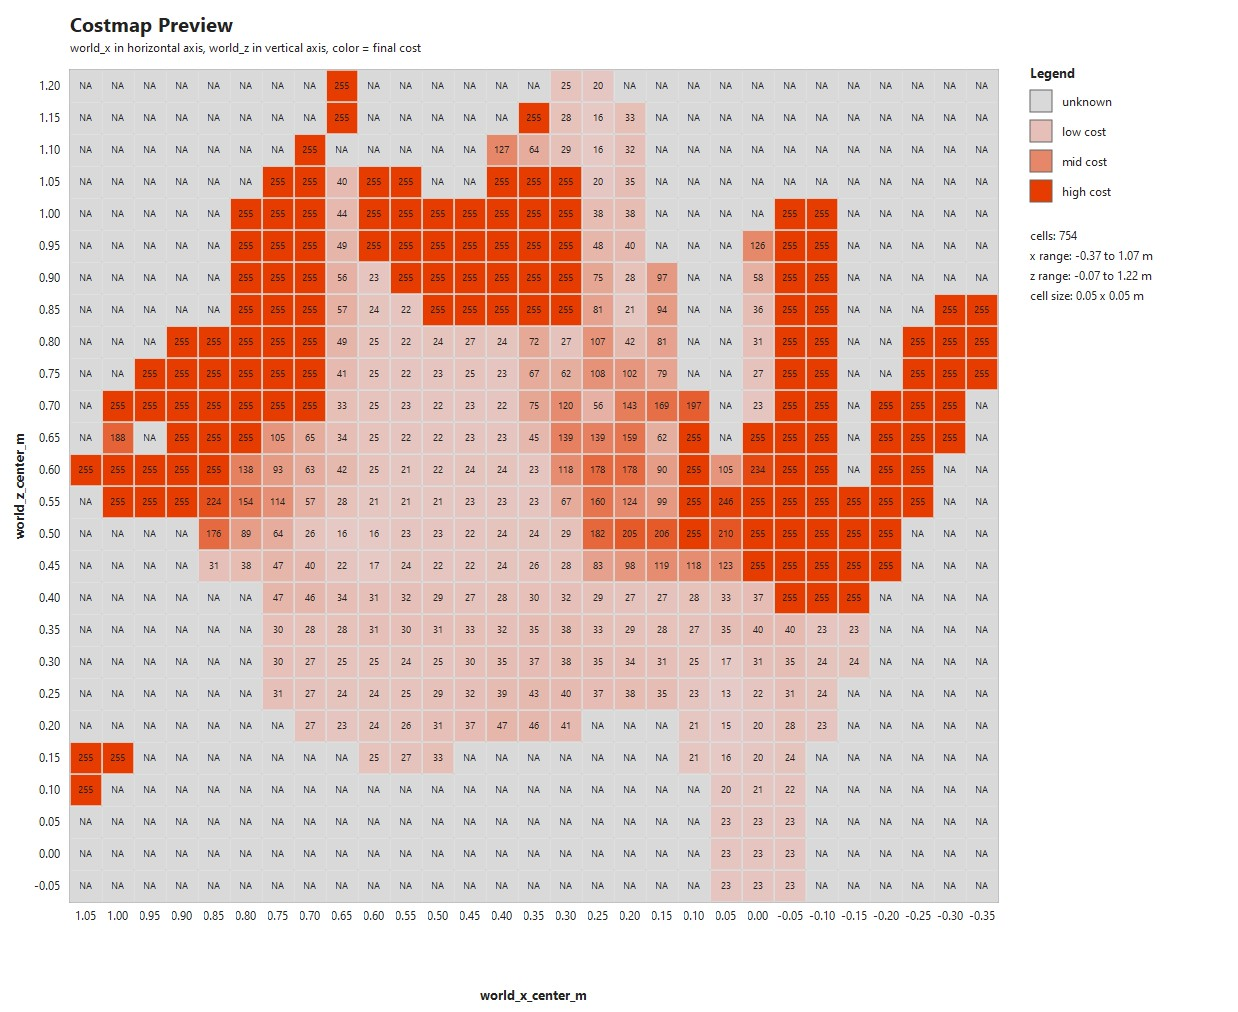
\includegraphics[width=\columnwidth]{figures/merge2dmap/5/map_costmap_view.jpg}
    \caption{Step 4}
    \label{fig:merge2dmap-step4}
\end{subfigure}
\caption{Overwrite-based global 2D map update during successive merging steps.}
\label{fig:merge2dmap-process}
\end{figure}

In the global map construction process, each grid cell is associated with its corresponding real-world coordinate. To save computational cost, each frame of map merging updates only the changed point-cloud data, and the 2D map module performs overwrite-based merging on the corresponding cells. This strategy is based on the assumption that, under ideal conditions, repeated point-cloud merging gradually reduces error and produces more accurate geometry. Therefore, newly observed results are used to overwrite previous ones. Through this mechanism, cells originally marked as \texttt{unknown} can also be updated into \texttt{costing} or \texttt{block}, allowing the global 2D map to evolve continuously during the scanning process. A typical overwrite-based update sequence is shown in Fig.~\ref{fig:merge2dmap-process}.

\subsection{Path Planning}
\label{subsec:path-planning-method-weijie-chen}

\subsubsection{Path-Planning Overview}

This path-planning module enables the robot to start from an unknown environment, gradually expand the known area, and use detected frontier regions as exploration targets until no frontiers remain in the map.

\subsubsection{Perception and Map Update}

The robot perceives the environment using an FOV model. Within its current facing direction, it uses multiple rays to obtain information about obstacles and traversable areas, and updates the occupancy grid map. At the same time, it performs local updates within a limited range around the robot to improve near-range perception accuracy. The hardware parameters used here are a camera field of view of \(45^\circ\), a perception range of 8 cells, and a grid size of 5\,cm.

To simulate perception delay in real systems, a \texttt{MapBuffer} is introduced in the code. During planning, the map from the previous frame is used for decision-making, reflecting the time gap between perception and processing in practical systems.

\subsubsection{Path Planning and Decision Making}

The input to the path-planning module consists of the cost map in \texttt{.npy} format provided by the mapping module, together with the robot's current world pose represented by \((x,z,\textit{yaw})\). The planner first converts the world pose into the corresponding grid position on the current map, and then uses the map cost and free/occupied information to generate the next motion decision.

The output of the planner is not a complete global trajectory, but an executable control sequence of the form
\[
\{(c_1,p_1),(c_2,p_2),\dots\}
\]
where the first element of each pair is the command type and the second is its parameter. In this system, \(0\) denotes stop, \(1\) denotes forward motion, \(2\) denotes backward motion, \(3\) denotes left rotation, and \(4\) denotes right rotation. The parameter is either the forward distance in cm or the rotation angle in degrees.

\begin{figure}[htbp]
\centering
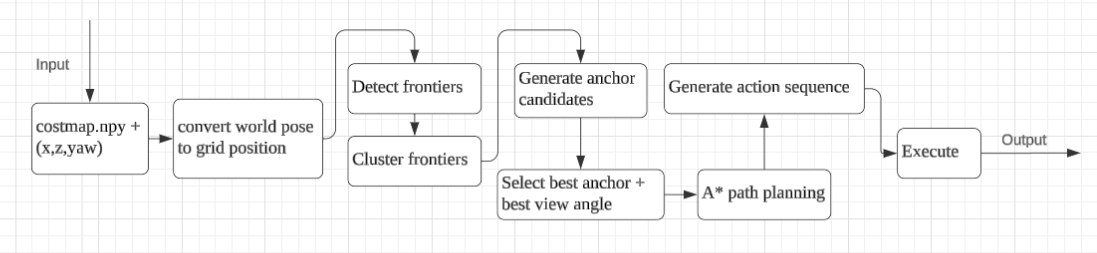
\includegraphics[width=\linewidth]{figures/weijie/7.png}
\caption{Decision-making pipeline of the robot for each planning step.}
\label{fig:decision-flow-weijie}
\end{figure}

The system detects frontier regions near the edge of the current map and connects them into clusters based on 8-neighborhood connectivity. For each frontier region, multiple observation anchors are generated as candidate observation locations. The planner then evaluates these anchors under different viewing angles according to path length, turning cost, map cost, overlap, and anticipated information gain. Once the best anchor is selected, a modified \(A^*\) search computes the most feasible path from the current position to that anchor.

\subsubsection{Motion and Constraints}

The robotic system uses a single-step strategy with a maximum forward movement of 2 cells (10\,cm) per step, a maximum rotation of \(15^\circ\), one-cell obstacle inflation (5\,cm), and a minimum observation-overlap ratio of 0.35 in order to support map stitching.

At every step, the system balances whether to scan first or move first, so that the amount of information gained is considered together with the movement cost incurred in the same time interval.

\subsubsection{Multi-Robot Coordination}

The implemented system consists of a three-robot exploration framework, where all robots contribute to a shared global occupancy grid while performing sensing and decision-making independently.

\begin{figure}[htbp]
\centering
\begin{subfigure}{0.32\linewidth}
    \centering
    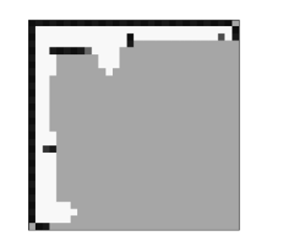
\includegraphics[width=\linewidth]{figures/weijie/8.png}
\end{subfigure}
\hfill
\begin{subfigure}{0.32\linewidth}
    \centering
    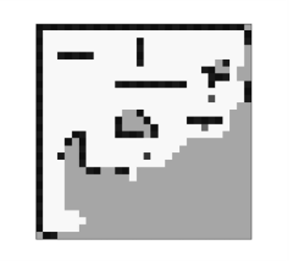
\includegraphics[width=\linewidth]{figures/weijie/9.png}
\end{subfigure}
\hfill
\begin{subfigure}{0.32\linewidth}
    \centering
    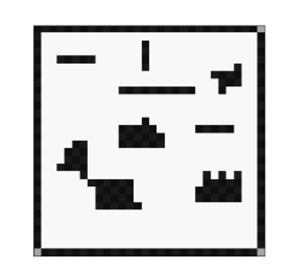
\includegraphics[width=\linewidth]{figures/weijie/10.png}
\end{subfigure}
\caption{Multi-robot exploration process over time.}
\label{fig:multi-robot-weijie}
\end{figure}

To coordinate the robots, the system uses target exclusion to avoid repeated frontier selection~\cite{ref1}, movement constraints and safe-distance rules for collision avoidance~\cite{ref2}, priority-based conflict resolution~\cite{ref3}, and field-of-view constraints to avoid visual interference~\cite{ref4}. A phased deployment strategy is also adopted so that robots enter the environment gradually rather than all at once~\cite{ref5}.

\subsubsection{Design Justification and Comparison with Existing Methods}

The path-planning module does not use complex optimization algorithms or learning-based methods. Instead, it adopts a cost-aware \(A^*\) strategy, which provides a good balance between computational efficiency and planning reliability under the present system setting.

Several commonly used strategies were compared, including \(A^*\)-based frontier exploration, random walk, DWA-like methods, VFH-like methods, and \(D^*\) Lite. As shown in Fig.~\ref{fig:comparison-side-weijie}, the \(A^*\)-based nearest-frontier method achieves near-complete coverage while requiring significantly fewer steps than most baseline methods.

\begin{figure}[H]
    \centering
    \begin{minipage}{0.48\linewidth}
        \centering
        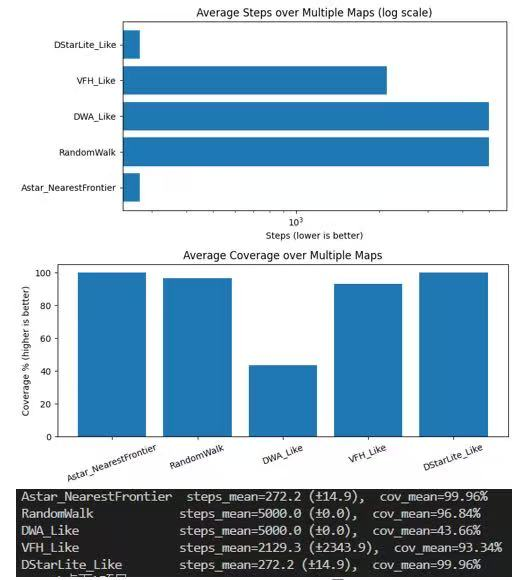
\includegraphics[width=\linewidth]{figures/weijie/1.jpg}
    \end{minipage}
    \hfill
    \begin{minipage}{0.48\linewidth}
        \centering
        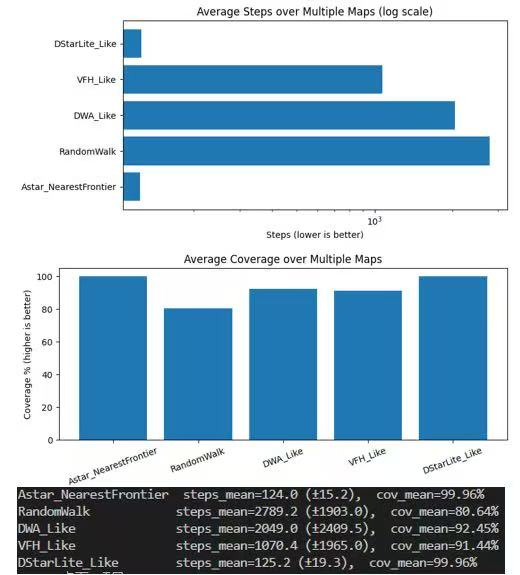
\includegraphics[width=\linewidth]{figures/weijie/2.jpg}
    \end{minipage}
    \caption{Comparison of exploration performance across different planning methods.}
    \label{fig:comparison-side-weijie}
\end{figure}

Computational performance was also evaluated in dynamic scenarios. As shown in Fig.~\ref{fig:time-comparison-weijie}, \(A^*\) requires significantly less total planning time than \(D^*\) Lite while maintaining comparable exploration performance.

\begin{figure}[H]
    \centering
    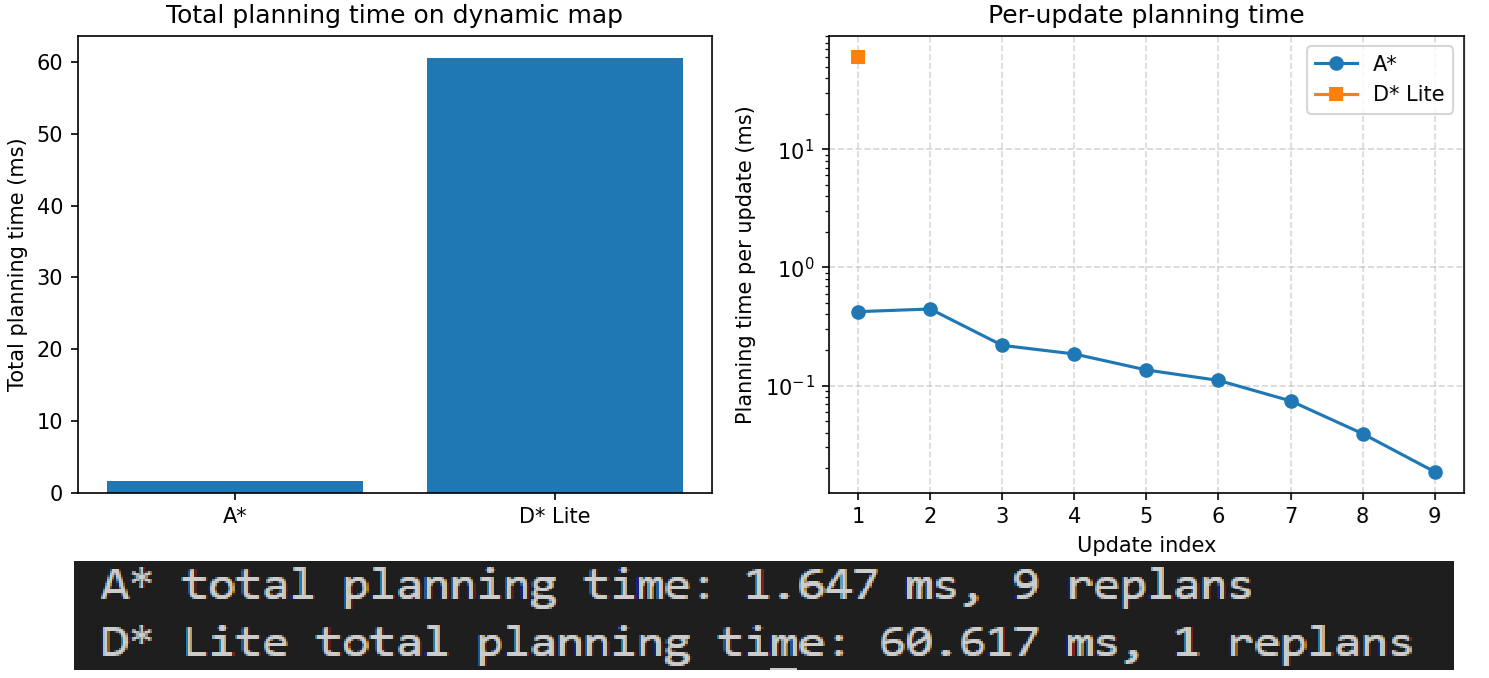
\includegraphics[width=0.8\linewidth]{figures/weijie/3.png}
    \caption{Comparison of total planning time and per-update planning time between \(A^*\) and \(D^*\) Lite in dynamic environments.}
    \label{fig:time-comparison-weijie}
\end{figure}

Compared with global optimization or distributed approaches, the current rule-based design is simpler to implement, easier to interpret, and more stable under limited computing resources. At the same time, the explicit inclusion of field-of-view constraints and a perception-delay model makes the planner more representative of real-world deployment conditions.



\section{Results, analysis, and discussion}

\subsection{Scanning Result Analysis}
\label{subsec:scanning-result-analysis-zhuyu-dong}



The scan result for the \(6.7\,\mathrm{m}^2\) real scene shows that, although the environment is somewhat cluttered and fragmented, the system is still able to represent the approximate spatial relationships among major objects. In overall terms, the reconstructed point cloud preserves the rough arrangement of obstacles and free space and therefore remains usable for subsequent map interpretation. Based on visual inspection of the reconstructed geometry, the practical error is approximately within \(\pm 5\text{--}10\,\mathrm{cm}/\mathrm{m}\).


\begin{figure}[htbp]
    \centering
    \begin{subfigure}[b]{0.4\columnwidth}
        \centering
        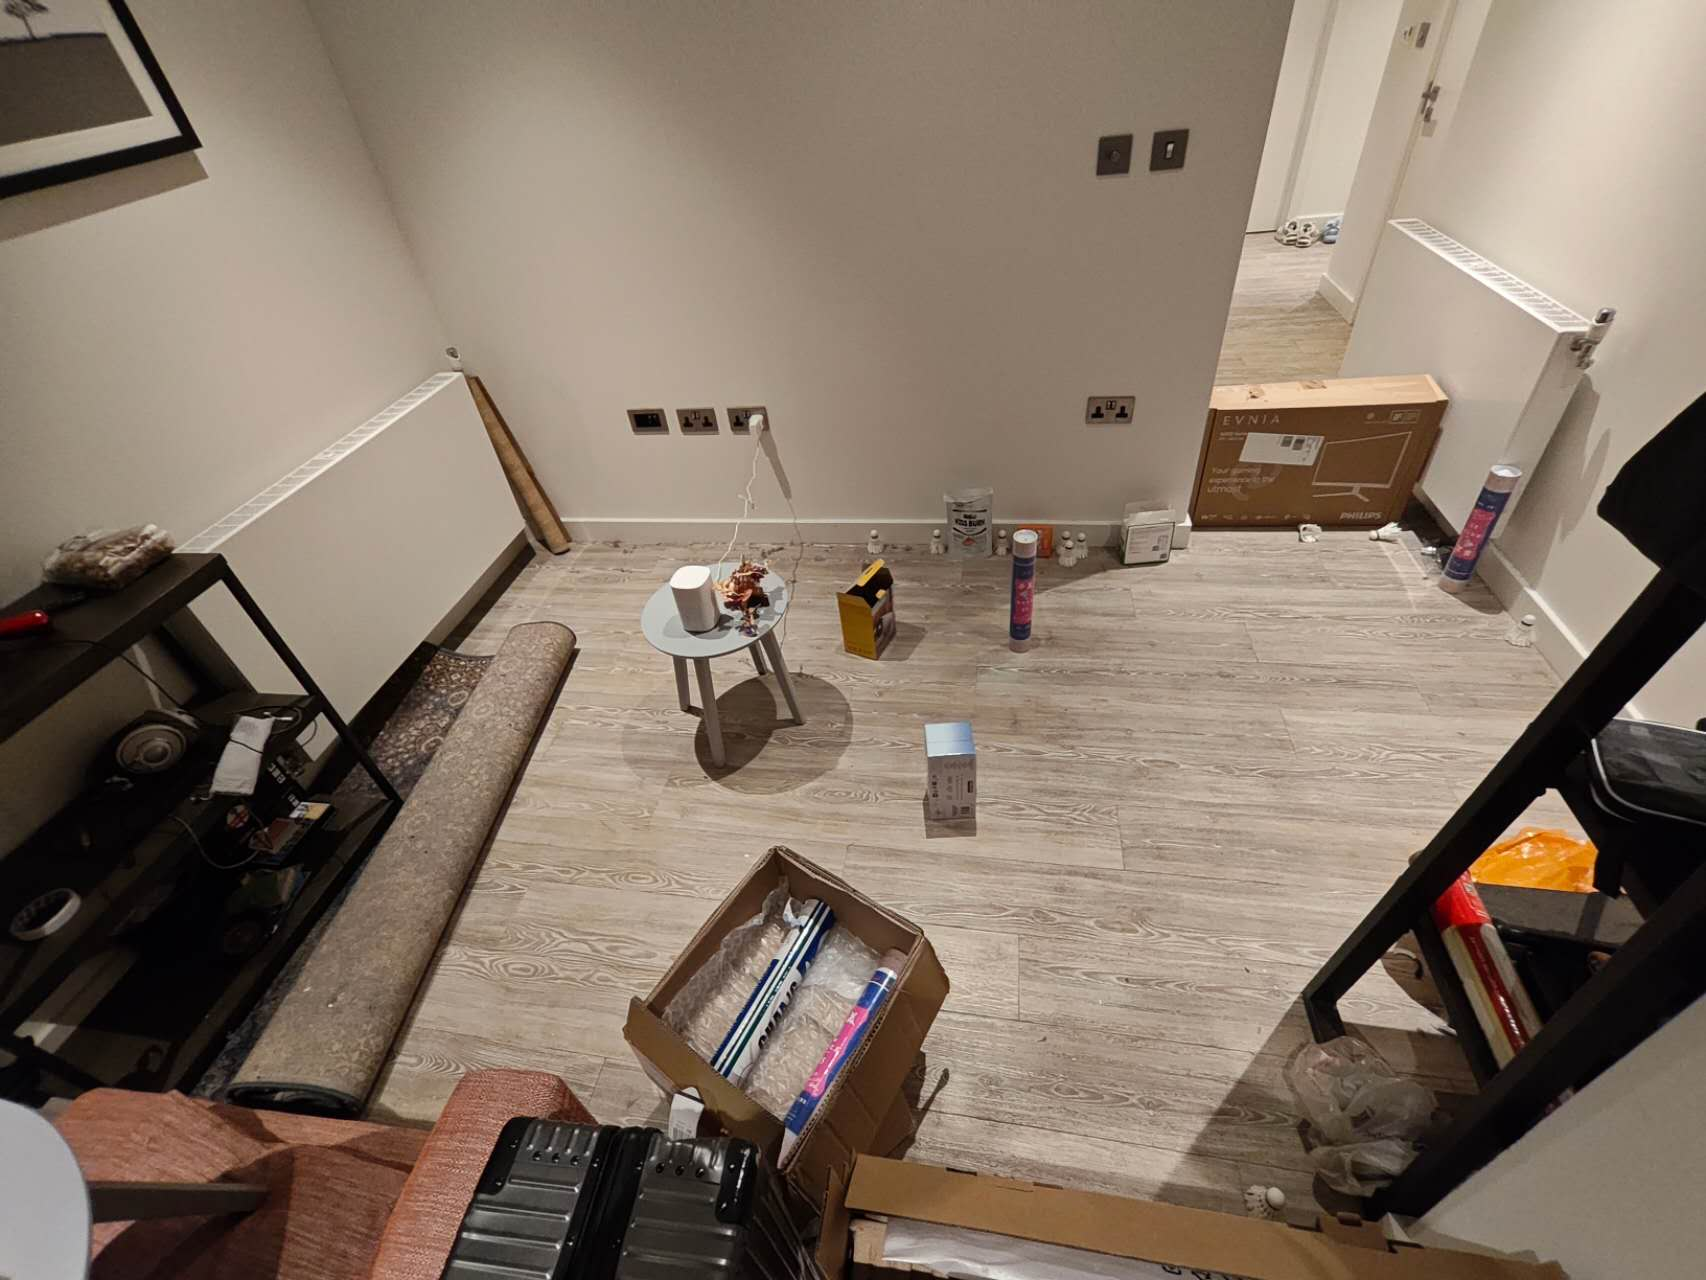
\includegraphics[width=\columnwidth]{figures/result/Reality.jpg}
        \caption{Real indoor scene.}
        \label{fig:result-reality}
    \end{subfigure}
    \hfill
    \begin{subfigure}[b]{0.48\columnwidth}
        \centering
        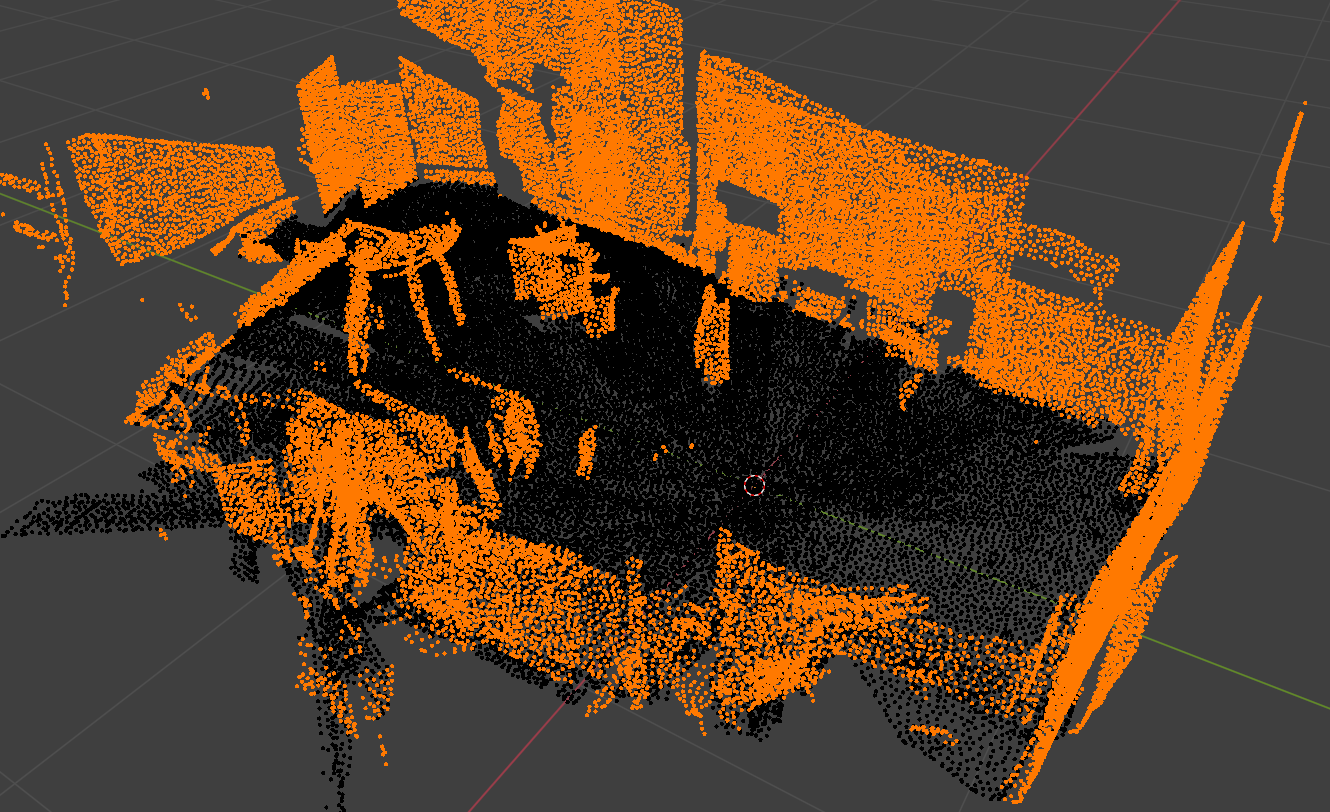
\includegraphics[width=\columnwidth]{figures/result/Point cloud of scan results.png}
        \caption{Point cloud of the scan result, where points above the ground layer are highlighted for clarity.}
        \label{fig:result-point-cloud}
    \end{subfigure}
    \caption{Comparison between the real scene and the reconstructed scan result.}
    \label{fig:result-scene-comparison}
\end{figure}

At the same time, several representative errors can be observed in the reconstructed result.

\begin{figure}[htbp]
    \centering
    \begin{subfigure}[b]{0.3\columnwidth}
        \centering
        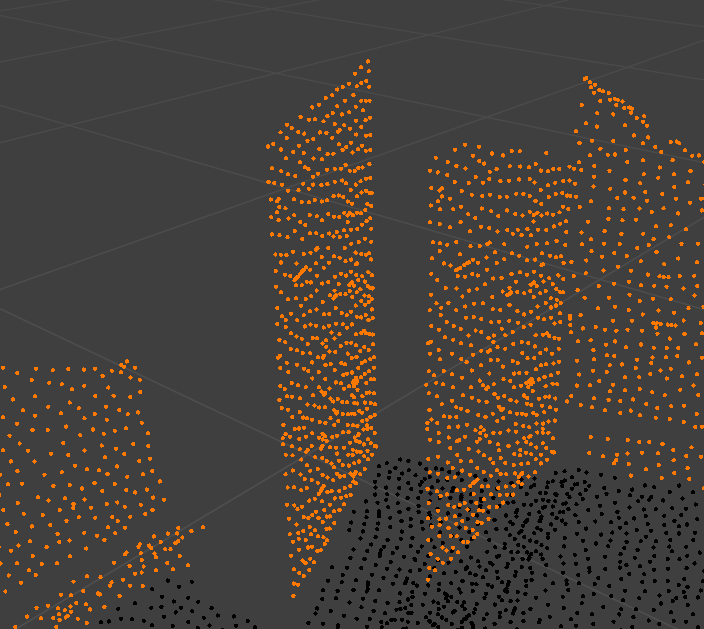
\includegraphics[width=\columnwidth]{figures/result/The Divided Wall.png}
        \caption{Point-cloud splitting.}
        \label{fig:result-divided-wall}
    \end{subfigure}
    \hfill
    \begin{subfigure}[b]{0.32\columnwidth}
        \centering
        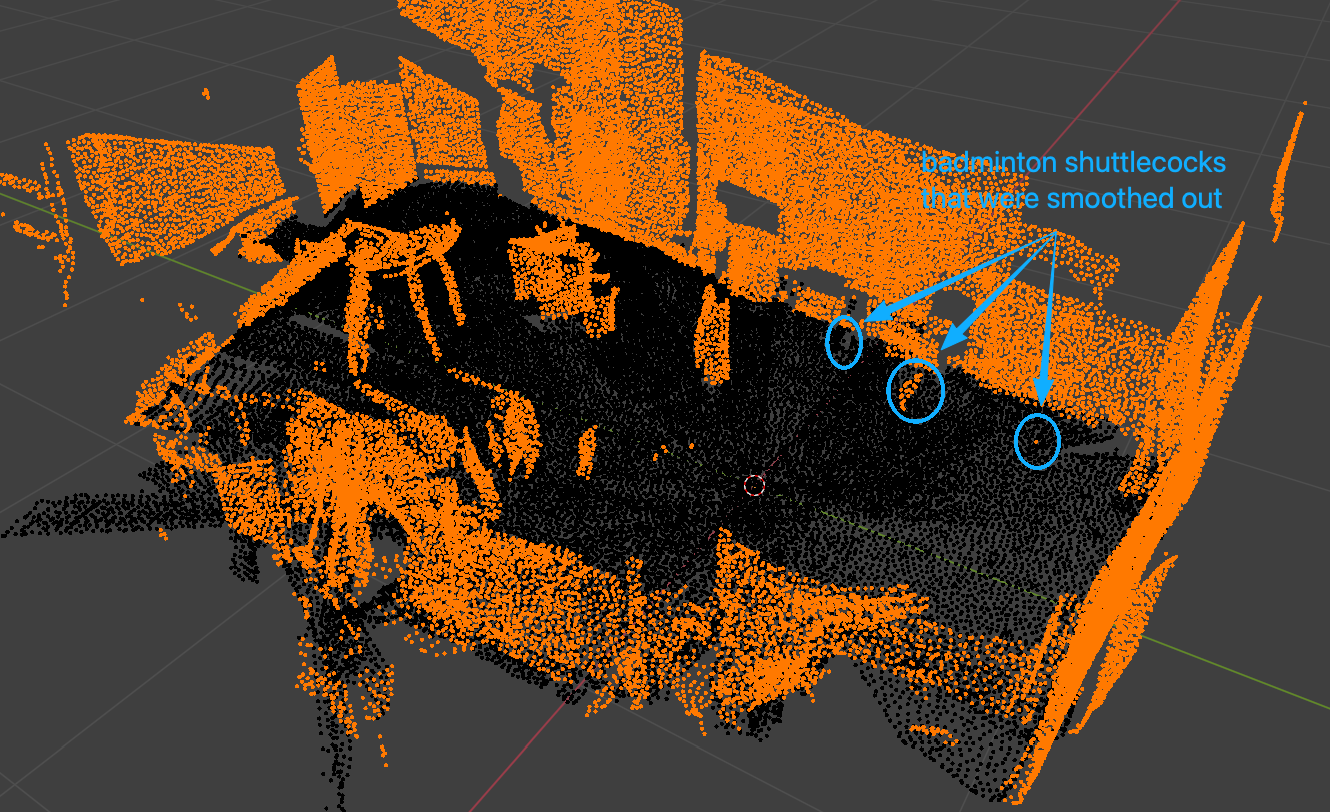
\includegraphics[width=\columnwidth]{figures/result/The badminton shuttlecock that was smoothed out.png}
        \caption{A small obstacle smoothed out during fusion.}
        \label{fig:result-smoothed-shuttlecock}
    \end{subfigure}
    \hfill
    \begin{subfigure}[b]{0.3\columnwidth}
        \centering
        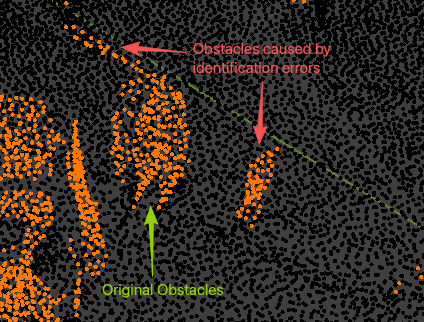
\includegraphics[width=\columnwidth]{figures/result/Obstacles caused by identification errors.png}
        \caption{False obstacles caused by identification errors.}
        \label{fig:result-false-obstacles}
    \end{subfigure}
    \caption{Representative reconstruction errors observed in the scan results.}
    \label{fig:result-error-cases}
\end{figure}

\begin{itemize}
    \item \textbf{Point-cloud splitting.} Parts of the same physical structure may fail to merge correctly. This issue mainly comes from three causes. First, the point-cloud conversion error for images taken at the same location may already be too large, so the corresponding local structures cannot be aligned reliably. Second, to preserve correct merging in other feature-rich areas, the global merging strategy may accept a compromise that leads to local merging failure. Third, when the robot moves with an overly large step size, the accumulated pose error becomes too large and the corresponding point clouds can no longer be merged consistently.

    \item \textbf{Small obstacles smoothed out.} If an obstacle is too small, or is too close to surrounding objects, or has visual features too similar to nearby structures, it may be absorbed into neighbouring geometry during the fusion process and therefore disappear from the reconstructed point cloud.

    \item \textbf{False obstacles generated by identification errors.} One cause is motion blur or poor image quality, which makes object boundaries in the estimated depth map unclear. This may create smooth but incorrect depth transitions around object edges, leading to wall-like point artifacts that cannot be removed cleanly by simple sharpening or truncation. Another cause is severe splitting in the merged point cloud, which may create unknown structures that are later interpreted as obstacles.
\end{itemize}

These error modes can also reinforce one another. When a small obstacle is smoothed out, reliable feature points become harder to detect, which increases the risk of further point-cloud splitting. Conversely, point-cloud splitting may introduce false local features, which can then cause even more splitting in subsequent merging steps. Similarly, falsely generated obstacles may also create artificial features and further destabilise later registration.

Overall, these problems are strongly related to changes in, or loss of, effective feature points. At a higher level, they mainly originate from two broader causes. One is excessive repeated capture at the same location: if point-cloud conversion already contains noticeable error, repeated observations may repeatedly reinforce the wrong geometry. The other is insufficient capture at the same location: if too few observations are collected, the system may fail to obtain clear and reliable information. Therefore, both too many and too few captures can be harmful. In practice, the most important factor is not simply the number of captures, but the accuracy of the image-to-point-cloud conversion itself, although this accuracy is difficult to guarantee consistently under real scanning conditions.

\subsection{Time Consumption and Pipeline Analysis}
\label{subsec:time-consumption-weijie-chen}

In the runtime environment, the central control host is equipped with an Intel i7-12700H CPU, an NVIDIA RTX 3060 GPU, and 24\,GB DDR5 (4800\,MHz) RAM. The execution time of each stage in the system, including robot control, image-to-point-cloud conversion, point cloud merging, 2D map projection, and path planning, is measured.

The average processing time per frame is approximately 18.09 seconds. Among all components, the most time-consuming stages are robot control, image-to-point-cloud conversion, and point cloud merging, as illustrated in Fig.~\ref{fig:single-frame-time-weijie}.

Although the overall processing time per frame is relatively high, the system benefits from the fact that different modules rely on different hardware resources. This makes it possible to use a pipeline-based parallel computation framework in multi-robot exploration. As shown in Fig.~\ref{fig:pipeline-weijie}, a new image is generated approximately every 7.72 seconds under the pipeline execution scheme, whereas purely sequential execution would require substantially more time.

\begin{figure}[htbp]
   \centering
   \begin{subfigure}{0.95\linewidth}
      \centering
      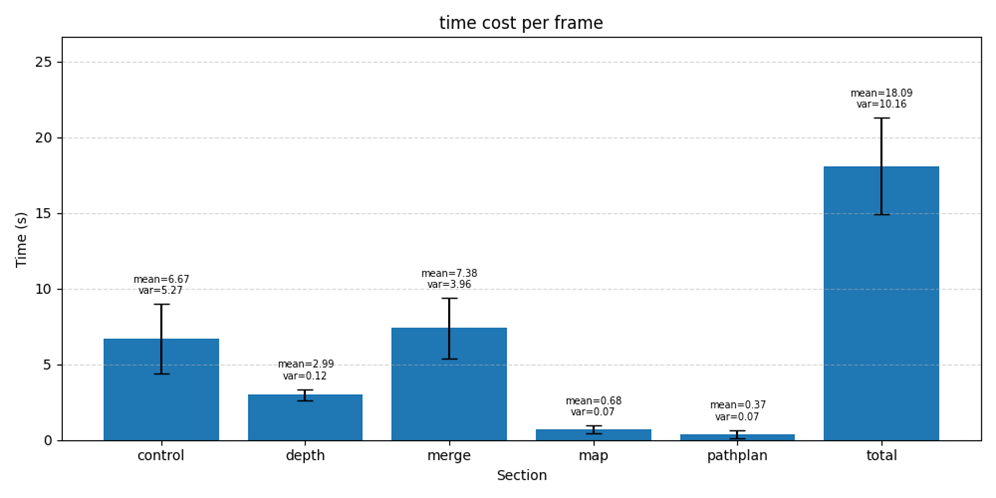
\includegraphics[width=\linewidth]{figures/weijie/11.png}
      \caption{Single-frame processing time for the five components of the system.}
      \label{fig:single-frame-time-weijie}
   \end{subfigure}
   \begin{subfigure}{0.95\linewidth}
      \centering
      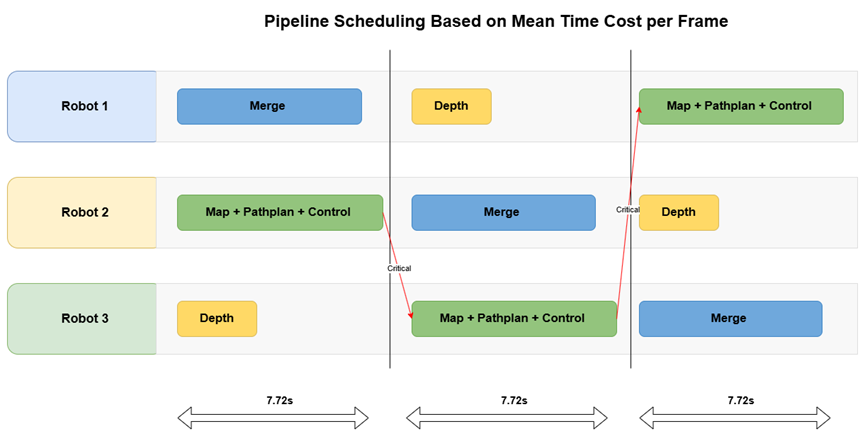
\includegraphics[width=\linewidth]{figures/weijie/12.png}
      \caption{Pipeline scheduling based on mean time cost per frame.}
      \label{fig:pipeline-weijie}
   \end{subfigure}
   \caption{Time-consumption and pipeline analysis of the system.}
   \label{fig:time-pipeline-overview-weijie}
\end{figure}

\subsection{Single-Robot Scene Scanning Experiment}
\label{subsec:single-robot-scanning-weijie-chen}

Four experimental environments used in this project are shown together in Fig.~\ref{fig:real-vs-costmap-overview-weijie}. Each scenario is constructed by progressively extending the base environment, with Scenario D further introducing an additional corner structure.

\begin{figure}[H]
    \centering
    \begin{subfigure}{0.2\linewidth}
        \centering
        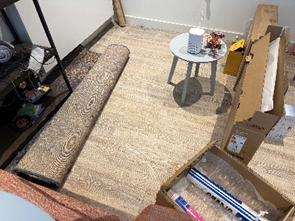
\includegraphics[width=\linewidth]{figures/weijie/rA.png}
        \caption{Scenario A: real-world scene (3$m^2$)}
    \end{subfigure}
    \hfill
    \begin{subfigure}{0.2\linewidth}
        \centering
        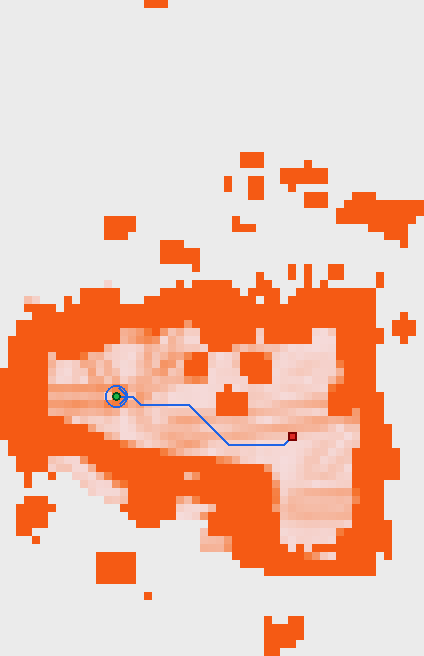
\includegraphics[width=\linewidth]{figures/weijie/cA.png}
        \caption{Scenario A: costmap and planned path}
    \end{subfigure}
    \hfill
    \begin{subfigure}{0.2\linewidth}
        \centering
        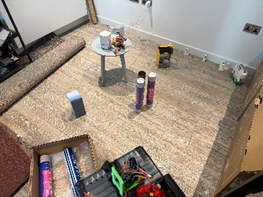
\includegraphics[width=\linewidth]{figures/weijie/rB.png}
        \caption{Scenario B: real-world scene (5.4$m^2$)}
    \end{subfigure}
    \hfill
    \begin{subfigure}{0.2\linewidth}
        \centering
        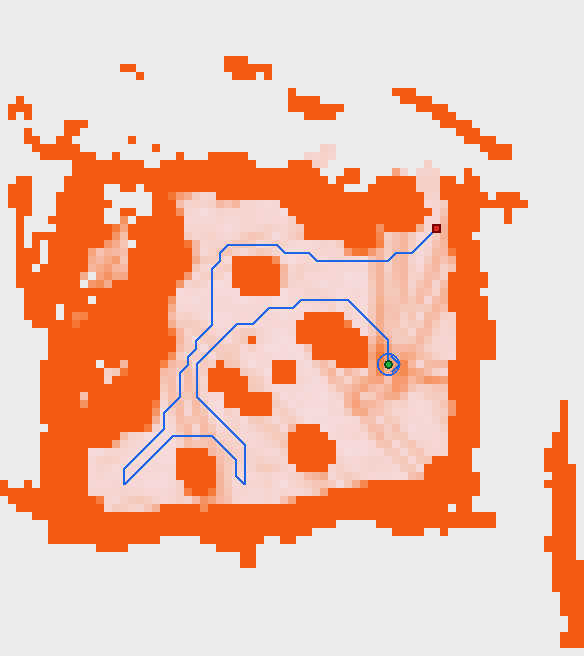
\includegraphics[width=\linewidth]{figures/weijie/cB.png}
        \caption{Scenario B: costmap and planned path}
    \end{subfigure}
    
    \vspace{0.8em}
    
    \begin{subfigure}{0.2\linewidth}
        \centering
        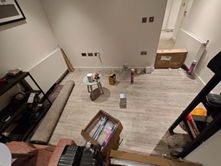
\includegraphics[width=\linewidth]{figures/weijie/rC.png}
        \caption{Scenario C: real-world scene (6.7$m^2$)}
    \end{subfigure}
    \hfill
    \begin{subfigure}{0.2\linewidth}
        \centering
        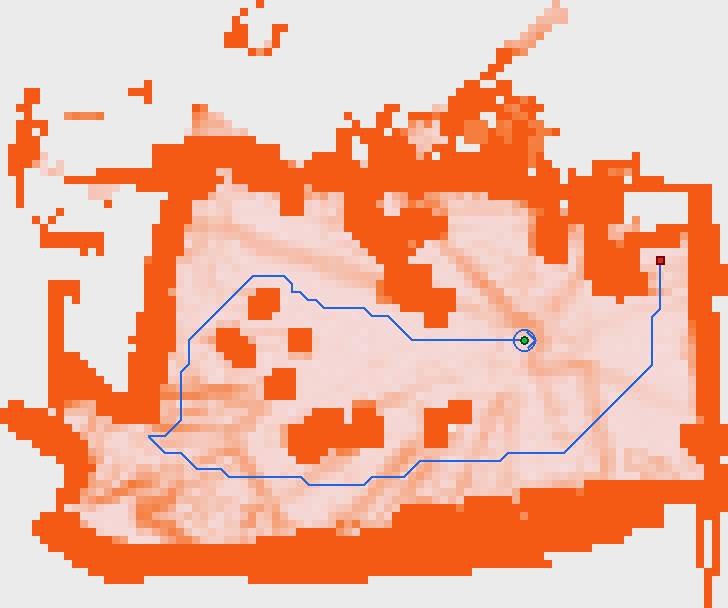
\includegraphics[width=\linewidth]{figures/weijie/cC.png}
        \caption{Scenario C: costmap and planned path}
    \end{subfigure}
    \hfill
    \begin{subfigure}{0.2\linewidth}
        \centering
        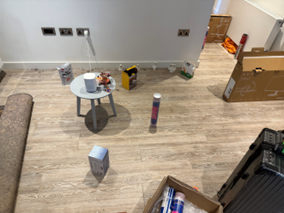
\includegraphics[width=\linewidth]{figures/weijie/rD.png}
        \caption{Scenario D: real-world scene (7.7$m^2$)}
    \end{subfigure}
    \hfill
    \begin{subfigure}{0.2\linewidth}
        \centering
        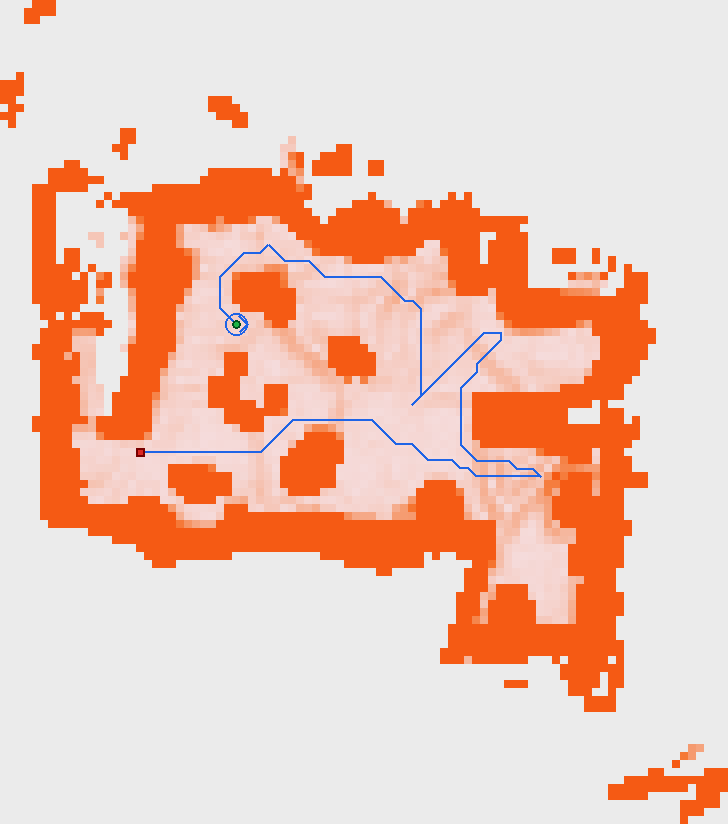
\includegraphics[width=\linewidth]{figures/weijie/cD.png}
        \caption{Scenario D: costmap and planned path}
    \end{subfigure}
    \caption{Comparison between the real-world scenes and the corresponding costmap-based path planning results across Scenarios A to D.}
    \label{fig:real-vs-costmap-overview-weijie}
\end{figure}

\begin{figure}[H]
    \centering
    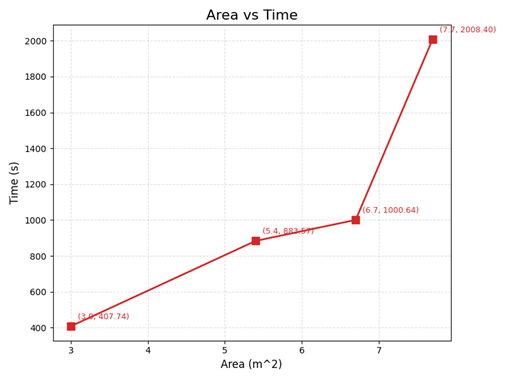
\includegraphics[width=0.48\linewidth]{figures/weijie/13.png}
    \hfill
    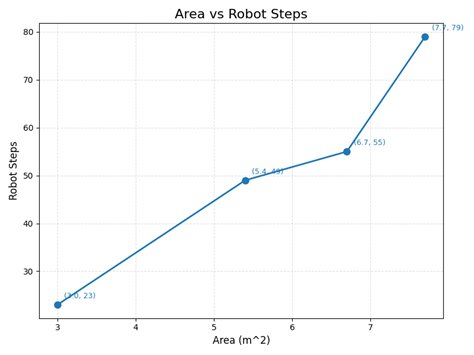
\includegraphics[width=0.48\linewidth]{figures/weijie/14.png}
    \caption{Relationship between environment area and (left) total scanning time, and (right) number of robot steps, where one step denotes one complete program cycle executed to capture a single photograph.}
    \label{fig:area-analysis-weijie}
\end{figure}

As shown in Fig.~\ref{fig:area-analysis-weijie}, the total scanning time is correlated with environment size, but not linearly. Scenario D shows a particularly large increase in total scanning time, mainly because the additional corner structure makes it harder for the robot to gather information and encourages more locally optimal decisions rather than globally efficient exploration.

\begin{figure}[H]
    \centering
    \begin{subfigure}{0.48\linewidth}
        \centering
        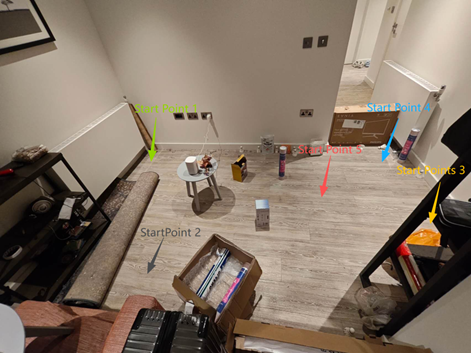
\includegraphics[width=\linewidth]{figures/weijie/15.png}
        \caption{Different initial positions of the robot in Scenario C.}
        \label{fig:start-points-weijie}
    \end{subfigure}
    \hfill
    \begin{subfigure}{0.48\linewidth}
        \centering
        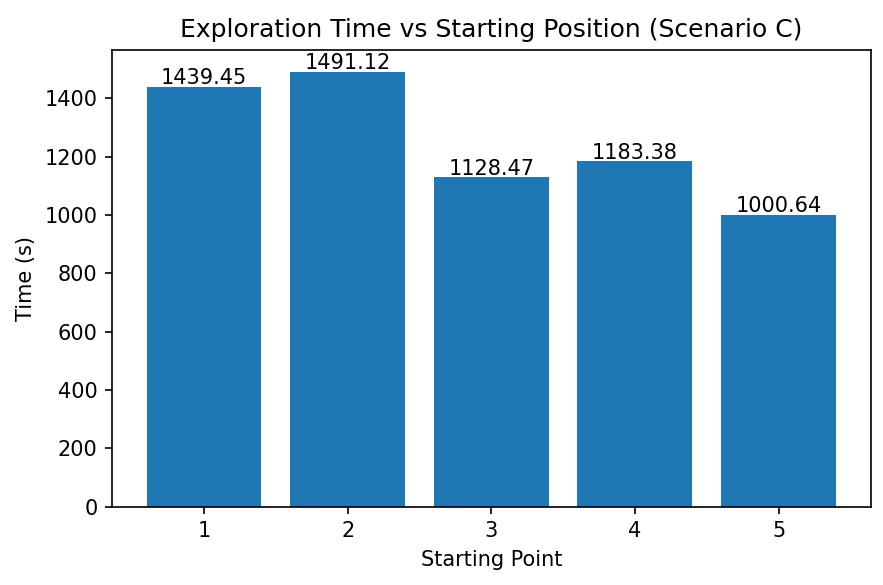
\includegraphics[width=\linewidth]{figures/weijie/16.png}
        \caption{Exploration time for different starting positions in Scenario C.}
        \label{fig:start-point-time-weijie}
    \end{subfigure}
    \caption{Influence of initial position on exploration performance in Scenario C.}
    \label{fig:start-point-analysis-weijie}
\end{figure}

The experiments also show that the initial robot position affects exploration efficiency. A starting point near the center allows the robot to observe a wider area early and acquire richer global information, leading to more effective planning. In contrast, starting positions in more constrained corners tend to increase redundant exploration and may even contribute to repeated scans and later point cloud fragmentation.

\subsection{Multiple Vehicles Scanning Simultaneously}
\label{subsec:multi-vehicle-scanning-weijie-chen}

As shown in Fig.~\ref{fig:comparison-time-vs-area-weijie}, the relationship between the number of vehicles and scanning speed is not linear. Instead, it exhibits diminishing marginal returns. This effect is especially pronounced in smaller environments, where the available area for independent exploration is limited and coordination overhead becomes dominant.

\begin{figure}[H]
    \centering
    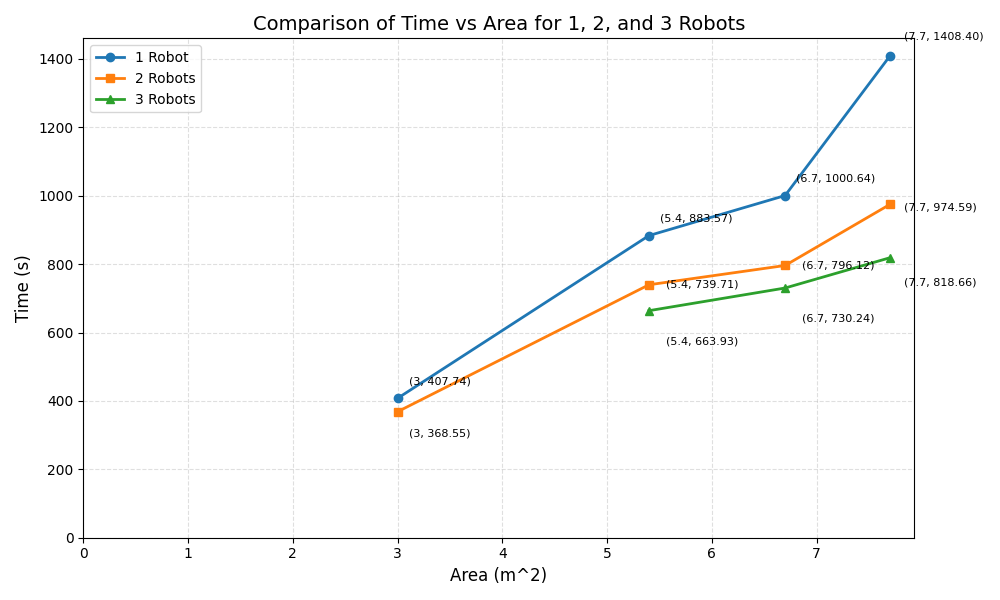
\includegraphics[width=0.9\linewidth]{figures/weijie/17.png}
    \caption{Comparison of time versus area for 1, 2, and 3 robots.}
    \label{fig:comparison-time-vs-area-weijie}
\end{figure}

In larger environments, however, the swarm-based multi-robot system has greater effective parallelization capacity. Because multiple robots can scan different subregions simultaneously with less mutual interference, the overall effective coverage per unit time increases, and richer global information is obtained for later path planning and task allocation.


\section{Conclusions and Future Work}

\subsection{Conclusion}
\label{subsec:overall-conclusion}

This project developed and integrated a low-cost multi-robot scanning system that connects image acquisition, monocular image-to-point-cloud reconstruction, point cloud merging, 2D map generation, and path planning into a complete end-to-end pipeline. The final system shows that useful environment reconstruction and exploration can be achieved without relying on expensive sensing hardware such as LiDAR, and that centralized processing can effectively support multiple small robots while keeping the hardware cost of each unit low.

From the experimental results, several key conclusions can be drawn. First, the image-to-point-cloud module is able to recover geometrically usable local structure within a practical near-field range, although accuracy degrades as distance increases. Second, the point cloud merging and 2D map stages can convert fragmented local observations into a map that is sufficient for traversability reasoning and later planning, but the final quality still depends strongly on point cloud consistency and feature stability. Third, the path-planning experiments show that the frontier-based cost-aware strategy is able to support both single-robot and multi-robot exploration, and that pipeline parallelism improves throughput in the multi-robot setting. At the same time, the results also reveal important limitations, including reconstruction error, local merging failure, false obstacles, single-layer map representation, and coordination overhead in denser multi-robot scenarios.

Overall, the project demonstrates the feasibility of combining monocular reconstruction, map fusion, and multi-robot path planning in a low-cost framework. However, it also shows that system-level performance is constrained not by a single module alone, but by the interaction between perception accuracy, fusion stability, map representation, and planning decisions. This makes the remaining gaps in the current system both practical engineering challenges and meaningful directions for further research.

\subsection{Future Work}
\label{subsec:future-work-qingzhou-zhang}

The most immediate future work is to improve the geometric reliability of the perception pipeline. The current results show that reconstruction accuracy decreases with distance and that unstable local geometry can later cause point cloud splitting, smoothing of small obstacles, and false obstacle generation. A key research question is therefore how to improve the consistency of monocular point cloud reconstruction across viewpoints while preserving fine local structure. Possible directions include scene-specific fine-tuning of the depth model, stronger post-processing of depth discontinuities, and more explicit confidence modeling during fusion.

The second major direction is to strengthen map representation and fusion scalability. The present system still relies on a single-layer 2D map and a fusion process whose computational cost grows with map size. This limits performance in vertically overlapping environments and in longer scanning sequences. Future work could investigate multi-layer map representations, chunk-based global map storage, and more efficient active-region or spatial-indexing strategies. These directions lead to a broader research question: how can a low-cost monocular system preserve global consistency while remaining computationally efficient in larger and more complex environments?

The third direction concerns planning and coordination. The current cost-aware frontier-based planner works effectively, but the experiments also show repeated paths, local-optimum behavior, and diminishing returns when robot density increases. Future work could therefore study more adaptive target scoring, incremental replanning, and global multi-robot task allocation. An especially important research question is how to balance information gain, overlap requirements, and coordination cost so that additional robots continue to produce meaningful improvements in exploration efficiency rather than mainly increasing system overhead.

More broadly, the results of this project suggest that future progress will depend on tighter coupling between perception, fusion, mapping, and planning rather than isolated optimization of a single module. For this reason, one promising research direction is to design closed-loop strategies in which reconstruction confidence, fusion uncertainty, and planning decisions are updated jointly, so that the system can actively choose motions that improve both map quality and exploration efficiency.



\section{Reference}
\bibliographystyle{ieeetr}
\bibliography{sample}

\section{Contribution}

\subsection{Roles of Team Members in the Project}

Zhuyu Dong:
\begin{itemize}
    \item Design and fabrication of two generations of robot platforms.
    \item Development of the onboard robot control software and the remote communication interface.
    \item Refactoring, improvement, and finalization of the point-cloud-to-2D-map module to ensure its successful integration into the overall system.
\end{itemize}

Junjie Ouyang:
\begin{itemize}
    \item Image-to-point-cloud reconstruction from captured photographs.
\end{itemize}

Qingzhou Zhang:
\begin{itemize}
    \item Point-cloud merging and fusion.
\end{itemize}

Chi Zou:
\begin{itemize}
    \item Feasibility-oriented technical exploration of point-cloud-to-2D-map conversion.
\end{itemize}

Weijie Chen:
\begin{itemize}
    \item Path planning for the multi-robot system.
\end{itemize}


\subsection{Subsections and Responsible Authors}

\begin{itemize}
    \item Introduction and Literature Review (Section 1) --- Weijie Chen, Zhuyu Dong, Junjie Ouyang
    \item \nameref{subsec:relative-pose-estimation-zhuyu-dong} (Section~\ref{subsec:relative-pose-estimation-zhuyu-dong}) --- Zhuyu Dong
    \item \nameref{subsec:image-to-point-cloud-junjie-ouyang} (Section~\ref{subsec:image-to-point-cloud-junjie-ouyang}) --- Junjie Ouyang
    \item \nameref{subsec:surface-fusion-qingzhou-zhang} (Section~\ref{subsec:surface-fusion-qingzhou-zhang}) --- Qingzhou Zhang
    \item \nameref{subsec:2dmap-theory-zhuyu-dong} (Section~\ref{subsec:2dmap-theory-zhuyu-dong}) --- Zhuyu Dong
    \item \nameref{subsec:path-planning-theory-weijie-chen} (Section~\ref{subsec:path-planning-theory-weijie-chen}) --- Weijie Chen
    \item \nameref{subsec:swarm-centralized-architecture-zhuyu-dong} (Section~\ref{subsec:swarm-centralized-architecture-zhuyu-dong}) --- Zhuyu Dong
    \item \nameref{subsec:robot-platform-zhuyu-dong} (Section~\ref{subsec:robot-platform-zhuyu-dong}) --- Zhuyu Dong
    \item \nameref{subsec:rtos-robot-control-zhuyu-dong} (Section~\ref{subsec:rtos-robot-control-zhuyu-dong}) --- Zhuyu Dong
    \item \nameref{subsec:image-to-point-cloud-method-junjie-ouyang} (Section~\ref{subsec:image-to-point-cloud-method-junjie-ouyang}) --- Junjie Ouyang
    \item \nameref{subsec:system-overview-mapper-pipeline-qingzhou-zhang} (Section~\ref{subsec:system-overview-mapper-pipeline-qingzhou-zhang}) --- Qingzhou Zhang
    \item \nameref{subsec:2dmap-generation-cost-modeling-zhuyu-dong} (Section~\ref{subsec:2dmap-generation-cost-modeling-zhuyu-dong}) --- Zhuyu Dong
    \item \nameref{subsec:path-planning-method-weijie-chen} (Section~\ref{subsec:path-planning-method-weijie-chen}) --- Weijie Chen
    \item Results, analysis, and discussion (Section 4) --- Weijie Chen, Zhuyu Dong, Junjie Ouyang, Qingzhou Zhang
    \item \nameref{subsec:future-work-qingzhou-zhang} (Section~\ref{subsec:future-work-qingzhou-zhang}) --- Qingzhou Zhang, Junjie Ouyang, Zhuyu Dong, Weijie Chen
    \item \nameref{subsec:first-generation-robot-zhuyu-dong} (Section~\ref{subsec:first-generation-robot-zhuyu-dong}) --- Zhuyu Dong
    \item \nameref{subsec:second-generation-robot-zhuyu-dong} (Section~\ref{subsec:second-generation-robot-zhuyu-dong}) --- Zhuyu Dong
    \item \nameref{subsec:bom-cost-estimate-zhuyu-dong} (Section~\ref{subsec:bom-cost-estimate-zhuyu-dong}) --- Zhuyu Dong
    \item \nameref{subsec:comparison-two-generations-zhuyu-dong} (Section~\ref{subsec:comparison-two-generations-zhuyu-dong}) --- Zhuyu Dong
    \item \nameref{subsec:junjie-appendix-image-to-point-cloud} (Section~\ref{subsec:junjie-appendix-image-to-point-cloud}) --- Junjie Ouyang
    \item \nameref{subsec:feature-coarse-registration-qingzhou-zhang} (Section~\ref{subsec:feature-coarse-registration-qingzhou-zhang}) --- Qingzhou Zhang
    \item \nameref{subsec:chizou-background} (Section~\ref{subsec:chizou-background}) --- Chi Zou
    \item \nameref{subsec:chizou-methods} (Section~\ref{subsec:chizou-methods}) --- Chi Zou
    \item \nameref{subsec:chizou-quantitative-analysis} (Section~\ref{subsec:chizou-quantitative-analysis}) --- Chi Zou
    \item \nameref{subsec:chizou-robustness-limitations} (Section~\ref{subsec:chizou-robustness-limitations}) --- Chi Zou
\end{itemize}






\appendix
\section{Hardware Iteration of the Robot Platform}
\label{app:hardware-iteration}

\subsection{First-Generation Robot}
\label{subsec:first-generation-robot-zhuyu-dong}

The first-generation robot shared the same overall goal as the final robot platform, but adopted a more function-heavy mechanical structure. Its main controller was an \texttt{ESP32-WROOM}, and the drive system used four \texttt{ULN2003} drivers with four \texttt{28BYJ-48} stepper motors to achieve forward, backward, leftward, and rightward motion. A single front universal wheel was used as the support structure. For image acquisition and active illumination, the robot employed an \texttt{OV3660} camera and four white LEDs. A dual-servo pan-tilt mechanism was further introduced to provide yaw and pitch adjustment of the camera, so that the robot could scan the environment from multiple viewing directions without changing the body orientation.

To obtain coarse pose feedback, the first-generation robot also included a rotational encoder module for translational distance estimation and an \texttt{MPU6050} IMU for angular feedback. In principle, this design offered relatively complete functionality. However, practical tests showed several shortcomings. The combination of stepper motors and gear sets occupied significant physical space, which caused the folded robot size to reach about \(25 \times 25 \times 15\text{ cm}\), and the working-state size to reach about \(25 \times 25 \times 35\text{ cm}\). Although this was still small compared with many conventional SLAM platforms, it was larger than desired for this project. Moreover, the \(1{:}2\) acceleration gear train pushed the stepper motors closer to their load limit, while the omni-wheel structure made slipping more likely and reduced the reliability of pose feedback. On sloped or uneven terrain, the four-wheel omni arrangement could also cause one wheel to lose effective contact with the ground, further reducing motion stability. In addition, the camera pitch mechanism introduced substantial depth-conversion error when images were captured from tilted viewpoints, which reduced the usefulness of such observations for later 3D reconstruction.

\begin{figure}[H]
    \centering
    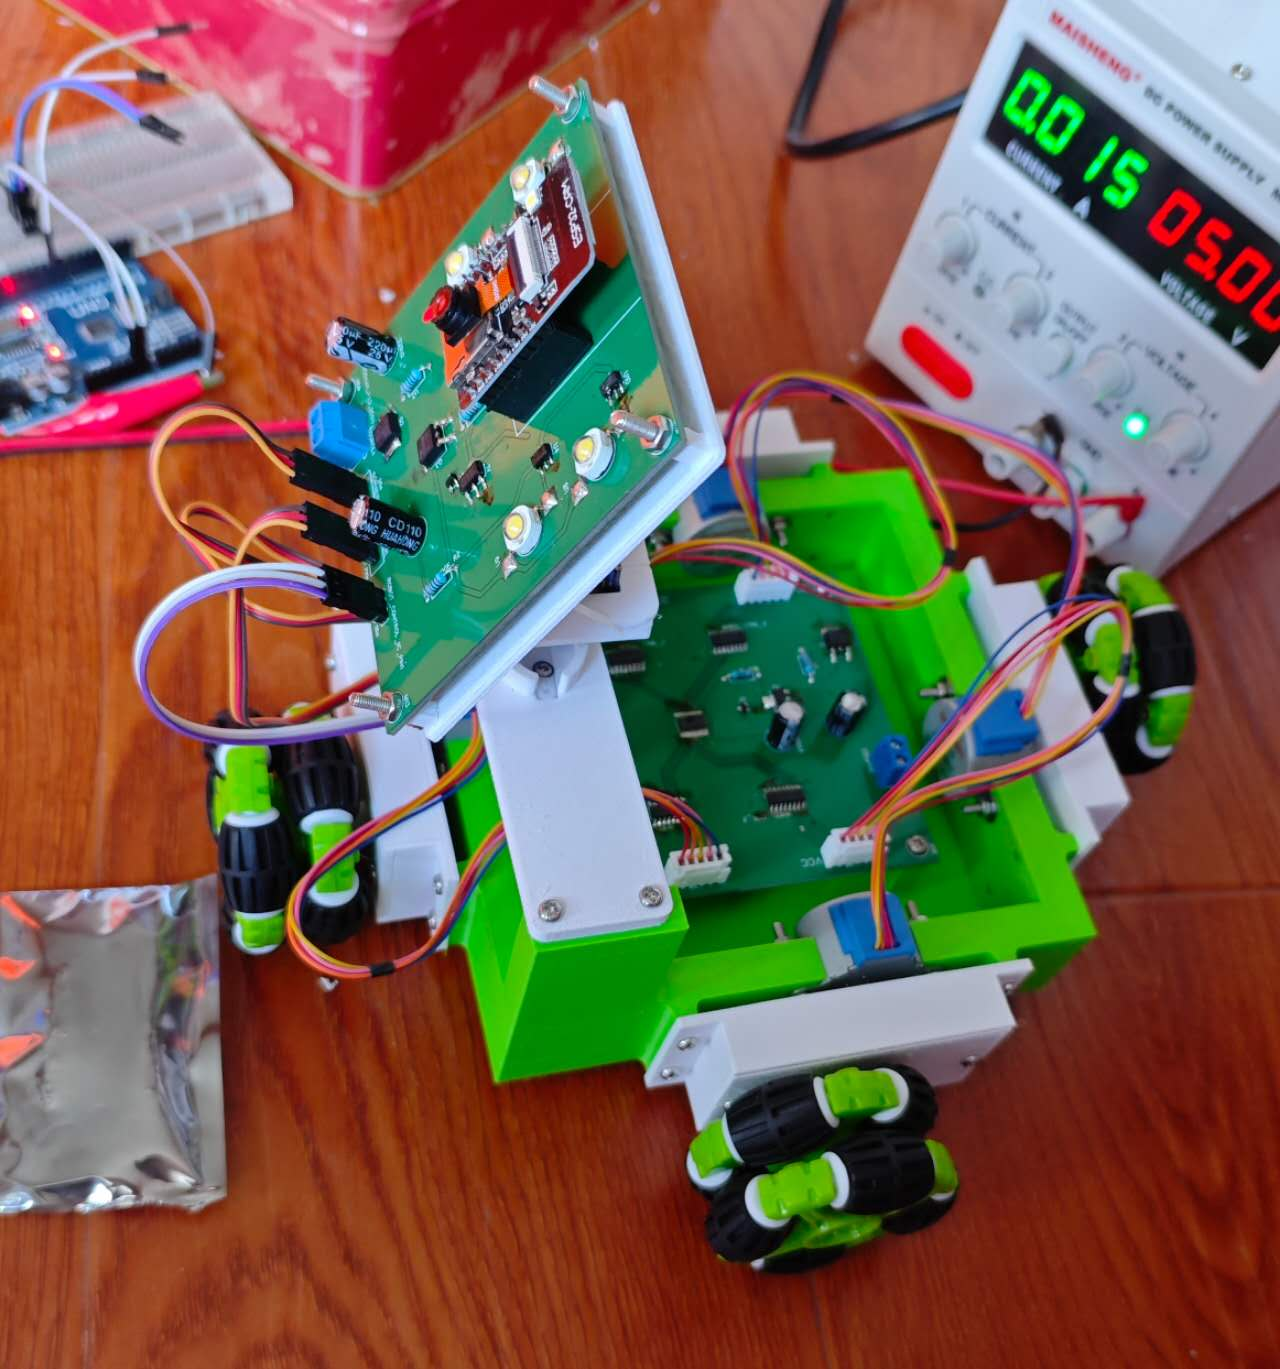
\includegraphics[width=0.8\columnwidth]{figures/car/v1.jpg}
    \caption{First-generation robot platform.}
    \label{fig:car-v1}
\end{figure}

\begin{figure}[H]
    \centering
    \begin{subfigure}[b]{0.48\columnwidth}
        \centering
        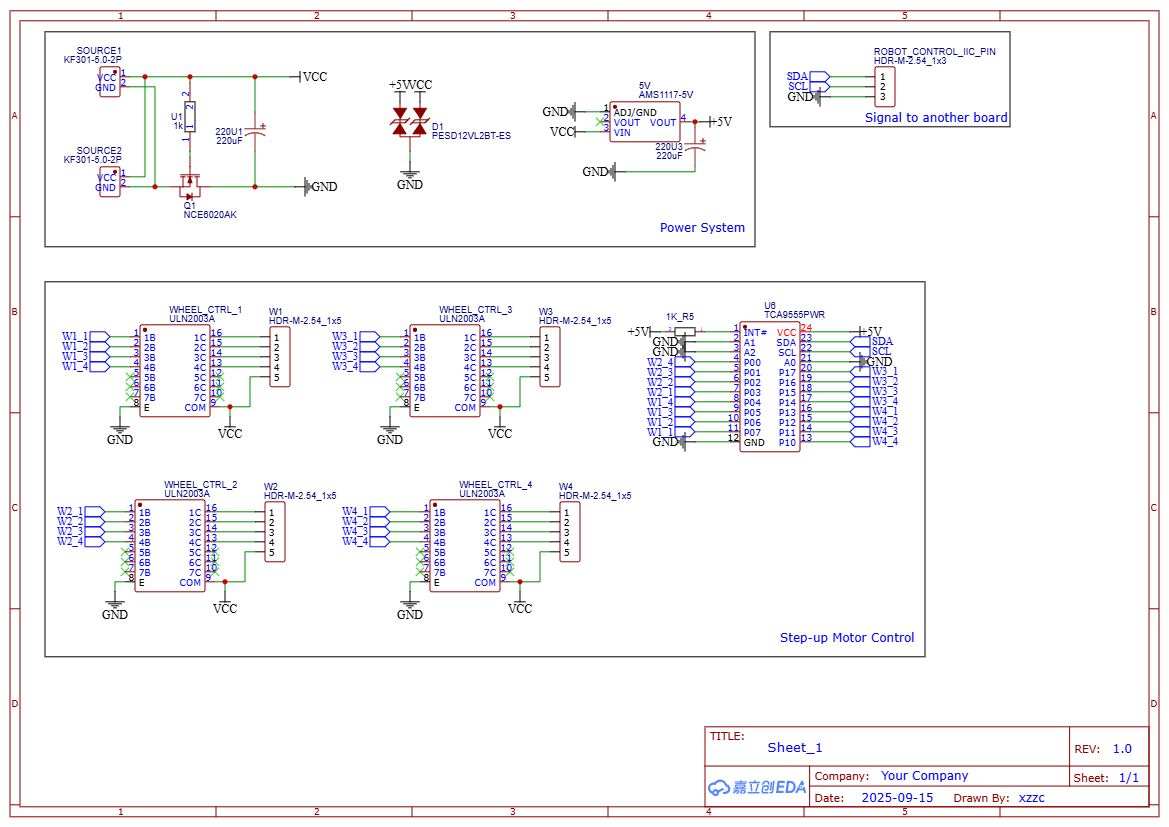
\includegraphics[width=\columnwidth]{figures/car/v1Body_sch.png}
        \caption{Body circuit.}
        \label{fig:car-v1-body-sch}
    \end{subfigure}
    \hfill
    \begin{subfigure}[b]{0.48\columnwidth}
        \centering
        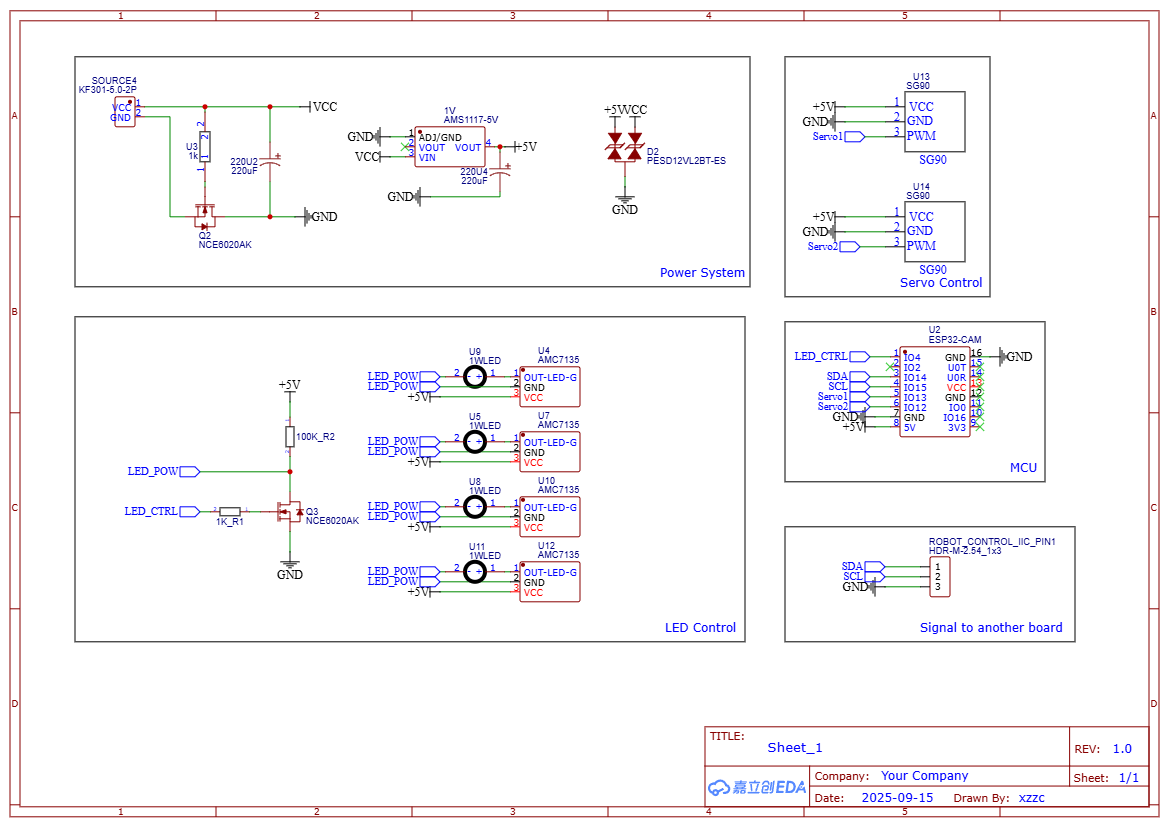
\includegraphics[width=\columnwidth]{figures/car/v1Head_sch.png}
        \caption{Head circuit.}
        \label{fig:car-v1-head-sch}
    \end{subfigure}
    \caption{Circuit schematics of the first-generation robot.}
    \label{fig:car-v1-sch}
\end{figure}

\subsection{Comparison Between the Two Generations}
\label{subsec:comparison-two-generations-zhuyu-dong}

Overall, the two robot generations reflect two different engineering trade-offs. The first-generation platform emphasised functional completeness, including lateral translation, camera pan-tilt control, and more auxiliary lighting, but this resulted in larger size, higher mechanical complexity, and poorer motion stability. The second-generation robot instead focused on preserving only the core functions required by the project, namely image capture, wireless communication, motion execution, and coarse pose estimation. Through this simplification, the second-generation design achieved better compactness, lower complexity, lower cost, and improved motion accuracy. For these reasons, the second-generation platform was selected as the final hardware platform used in this work.

\section{Image-to-Point-Cloud Reconstruction Appendix}
\label{app:junjie-image-to-point-cloud}

\subsection{Image-to-Point-Cloud Reconstruction}
\label{subsec:junjie-appendix-image-to-point-cloud}

The main implementation file for this submodule is \texttt{Final 1280.py}. This file contains the core functions used in this part of the work, including depth estimation, point cloud reconstruction, post-processing, and output generation. It is the main code file used to produce the results presented in this report.

The writing process related to this part of the report is documented in the following repository:

\begin{quote}
\texttt{https://github.com/nuanzhi6666/writing}
\end{quote}

This repository contains the writing history of this section, including early drafts, revised versions, and the final written form used in the report. AI tools were used only for grammar checking, correction of language errors, and polishing of wording. The technical ideas, implementation decisions, experimental work, and core written content of this part were developed by the author.

\section{Feature Coarse Registration}
\label{subsec:feature-coarse-registration-qingzhou-zhang}

The colour-assisted coarse registration module is designed to provide a more reliable initial alignment for subsequent fine registration. The underlying algorithm is based on coarse registration using local geometric descriptors such as FPFH. Conventional coarse registration primarily establishes candidate correspondences based on local geometric distributions of point clouds. However, when the geometric structure of the input point clouds is distorted, relying solely on geometric features may lead to incorrect matches.

To mitigate this issue, the proposed system introduces a colour consistency constraint on top of geometric feature matching, incorporating local colour statistics as additional discriminative information. Specifically, point cloud colours are first transformed into the Lab colour space, and the $a$ and $b$ channels are extracted as colour descriptors. Compared with the RGB space, the Lab-$ab$ space reduces the influence of illumination variations on matching.

In terms of implementation, the system first performs voxel downsampling with a relatively large voxel size on both the source and target point clouds, followed by normal estimation and FPFH feature computation, in order to construct a sparse set of feature points for coarse registration. Subsequently, for each feature point, the system computes the mean and variance of the Lab-$ab$ colour values within its local neighbourhood, which serve as local colour statistical descriptors.

Candidate correspondences are initially generated based on distances between FPFH geometric features and are further filtered using bidirectional consistency, retaining only mutually selected point pairs. On this basis, the system further evaluates the differences in local colour means and variances between candidate pairs, removing matches with excessive colour discrepancies. The geometric distance and colour difference are then combined through a weighted formulation to re-rank the candidate correspondences.

Finally, a ratio test is applied to eliminate ambiguous matches, and the filtered correspondences are fed into RANSAC to estimate the initial rigid transformation. This design preserves the global search capability of geometric features while enhancing the discriminative power of candidate correspondences through colour information, thereby reducing the risk of mismatches caused by repetitive structures or locally similar geometries.

However, due to unsatisfactory performance observed during experimental evaluation, this module was not enabled in the final system.
\section{Experimental Point-Cloud-to-2D Map Techniques}
\label{app:chi-zou-2dmap}

This appendix summarizes an experimental point-cloud-to-2D map pipeline developed by Chi Zou. The methods explored in this part focus on converting sparse monocular depth point clouds into semantic and cost-based 2D maps. These techniques were investigated as supporting experiments, but were not incorporated into the final onboard robot workflow used in the main system.

\subsection{Theoretical, Mathematical and Scientific Background}
\label{subsec:chizou-background}

\subsubsection{Theoretical Basis of 2D Grid-Based Terrain Representation}
\label{subsec:chizou-grid-terrain-theory}

In mobile robot navigation, although raw 3D point clouds provide a lot of spatial geometric information, performing passability assessments and path planning directly within the full 3D space typically involves processing complex data, leading to high computational costs and long waiting times. Therefore, many studies choose to compress 3D maps into 2D or 2.5D grids, to reduce the complexity of planning and analysis by retaining the topographical information most relevant to movement decisions~\cite{meng2018terrain,sanchez2019pff}.

\subsubsection{Mathematical Definitions of Terrain Geometric Features}
\label{subsec:chizou-geometric-features}

In this project, the two-dimensional grid is considered the basic statistical unit for estimating geometric features, rather than simple spatial discretisation units. For each grid cell, the system extracts various geometric features from the near-surface point cloud, including elevation difference, slope and roughness, to assess surface topography and flatness~\cite{meng2018terrain,carvalho2024traversability}.

The following describes how the project processes these geometric features.

\begin{itemize}
    \item Define the average height near the surface \texttt{mean\_z} as:
    \begin{equation}
        \mathrm{mean\_z} = \frac{\sum z_i}{N_g}
    \end{equation}
    where $N_g$ represents the number of points in a given grid that are classified as belonging to the ground layer.

    \item The elevation difference between cells \texttt{elev\_diff} is defined as
    \begin{equation}
        \mathrm{elev\_diff} = z_{\max} - z_{\min}
    \end{equation}

    \item The roughness is defined as the standard deviation of the elevation of near-surface points
    \begin{equation}
        \mathrm{roughness} = \sqrt{\max\!\left(\frac{\sum z_i^{2}}{N_g} - \mu^{2},\; 0\right)}
    \end{equation}
    $\mu$ is the average elevation of near-surface points in the current grid.

    \item Slope is defined from the gradient of the elevation map. In the script, the \texttt{mean\_z} map is first filled with NaN values, and \texttt{np.gradient} is then used to compute the two directional gradients $g_x$ and $g_y$.
    \begin{equation}
        \mathrm{slope} = \arctan\!\left(\sqrt{g_x^{2} + g_y^{2}}\right)
    \end{equation}
    NaN is used to mark missing grid cells where no valid ground data is available, and \texttt{np.gradient} is used to calculate the discrete gradients in two spatial directions for the interpolated elevation map.

    \item The script also uses \texttt{above\_count} to record how many points lie above each grid cell, helping distinguish near-surface obstacles from higher structures.
\end{itemize}

\subsubsection{Theoretical Basis of Semantic Traversability Classification}
\label{subsec:chizou-semantic-traversability}

To make the map easier for robot path planning, this study divides the two-dimensional grid into three categories using semantic labels: UNKNOWN, EXPLORABLE, and BLOCKED~\cite{sanchez2019pff,carvalho2024traversability}.

UNKNOWN indicates that there is insufficient observational evidence for the current grid cell; EXPLORABLE means the area has been observed and no explicit obstacles have been detected; and BLOCKED represents the existence of strong geometric evidence proving that the area is not passable.

This three-category classification design is derived from the inherent uncertainty in single-frame depth point clouds, where missing observations, sparsity and noise can lead to certain areas that cannot be classified as either vacant or occupied.

\subsubsection{Mathematical Criteria for Hard Blocking}
\label{subsec:chizou-hard-blocking}

In this study, the BLOCKED area is not defined directly by a single threshold but rather consists of several confirmed hazards. The core theoretical principle is that a grid cell should only be considered non-traversable when it is supported by sufficiently strong geometric evidence~\cite{sanchez2019pff}.

In the code, the final hard block is composed of the following combination:
\begin{equation}
    \mathrm{blocked} = \mathrm{obstacle\_core} \ \vee\ \mathrm{inflated} \ \vee\ \mathrm{step\_edge}
\end{equation}

\begin{itemize}
    \item \texttt{obstacle\_core} describes distinct vertical obstacles. A grid cell is assigned to this term when it lies in a well-observed area, its \texttt{above\_count} reaches the minimum obstacle-count threshold, and its maximum near-surface height exceeds the obstacle-height threshold.

    \item The method uses 8-neighbour support to identify cells whose height differs sharply from several surrounding cells. If this support condition is satisfied, the grid cell is considered a hazardous edge area.
    \begin{equation}
        |\Delta z| > h_{\mathrm{step}}
    \end{equation}

    \item \texttt{inflated} is the safety expansion of \texttt{obstacle\_core}, used to represent the robot's physical dimensions and safety margin so that planned paths do not pass too close to obstacle boundaries.
\end{itemize}

\subsubsection{Theoretical Basis of Continuous Traversability Cost}
\label{subsec:chizou-continuous-cost}

Hard-block reasoning is insufficient for path planning, because traversal difficulty still varies within passable areas. Therefore, this study introduces a continuous traversability cost to represent the relative difficulty of movement within EXPLORABLE regions~\cite{carvalho2024traversability}.

For the EXPLORABLE region, the cost is defined as:
\begin{equation}
    C = w_s S + w_r R + w_e E + w_p \exp(-d/\lambda)
\end{equation}

\begin{itemize}
    \item $w_x$ is the weighting factor in the total cost.
    \item $S$ is the normalized slope.
    \item $R$ is the normalized roughness.
    \item $E$ is the normalized elevation difference within a single cell.
    \item $d$ is the Euclidean distance from the current grid to the nearest BLOCKED grid.
    \item $\lambda$ is the distance decay parameter.
    \item The proximity term $\exp(-d/\lambda)$ applies a higher penalty near obstacle boundaries and decreases with distance, encouraging safer paths away from hazardous regions~\cite{chen2022gpu}.
\end{itemize}

\subsubsection{Rationale for Separating Hard Block and Soft Cost}
\label{subsec:chizou-hard-soft-separation}

A key design principle of this study is the explicit separation between hard block and soft cost. Hard block is used to determine whether an area is absolutely non-traversable, while soft cost is used to describe the relative traversal difficulty within traversable regions. This design allows the map to represent not only whether a region can be crossed, but also how difficult it is to traverse~\cite{carvalho2024traversability}. Figure~\ref{fig:chizou-traversability} gives a visual comparison of these two layers.

\begin{figure}[H]
    \centering
    \makebox[\linewidth][c]{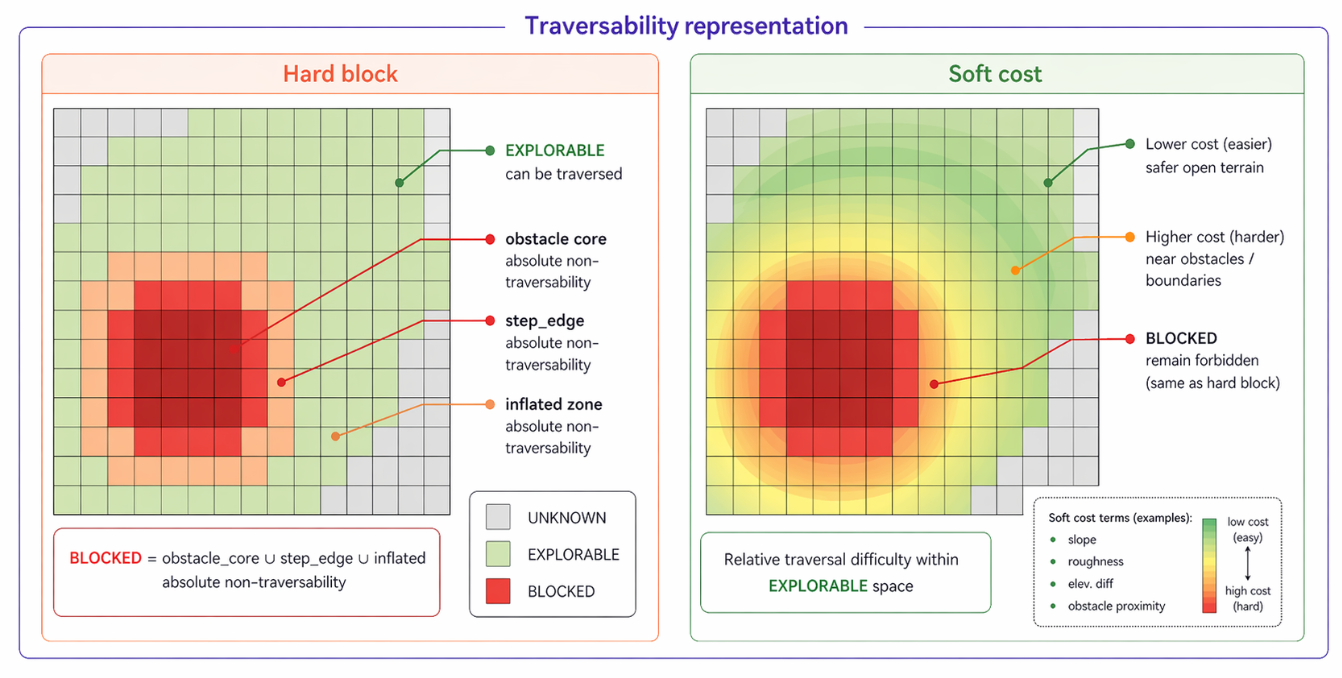
\includegraphics[width=0.9\linewidth]{figures/chizou/traversability.png}}
    \caption{Hard block and soft cost in traversability mapping.}
    \label{fig:chizou-traversability}
\end{figure}

This separation is particularly important for depth-derived point clouds, which are often affected by noise. Since slope is computed from the gradient of a 2D elevation map, it is sensitive to local height errors. If slope is used directly as a hard blocking criterion, traversable areas may be incorrectly marked as blocked. For this reason, the present study restricts BLOCKED regions to confirmed obstacle core, step edge, and their inflated zones, while slope, roughness, and \texttt{elev\_diff} are retained as soft cost terms in the continuous cost map. In this way, the system reduces over-blocking caused by noise while still preserving the ability to represent local terrain complexity.

\subsection{Methods, Setups and Software Implementation}
\label{subsec:chizou-methods}

\subsubsection{Implementation Pipeline}
\label{subsec:chizou-implementation-pipeline}

This experimental implementation converts local point clouds into 2D maps in three stages: the input point cloud is preprocessed and rasterized, a semantic map is generated from near-surface analysis and local geometric features, and a continuous traversability cost map is then constructed.

\begin{figure}[H]
    \centering
    \makebox[\linewidth][c]{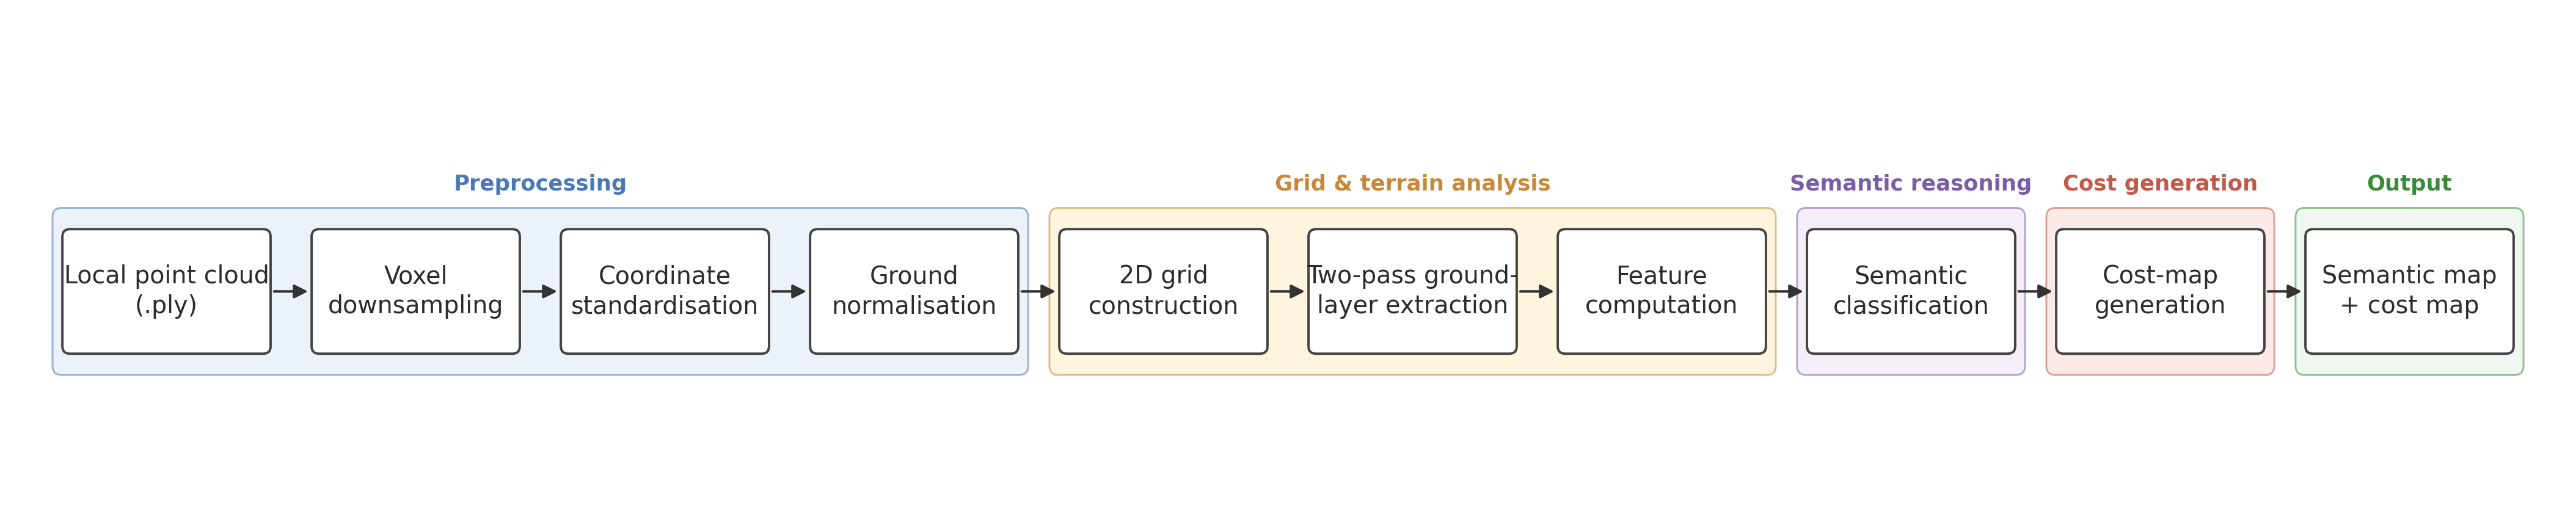
\includegraphics[width=0.9\linewidth]{figures/chizou/pipeline.png}}
    \caption{Overview of the proposed pipeline for converting local point clouds into semantic and cost-based 2D maps.}
    \label{fig:chizou-pipeline}
\end{figure}

\subsubsection{Point-Cloud Preprocessing and Grid Representation}
\label{subsec:chizou-preprocessing-grid}

This section takes a \texttt{.ply} point cloud file as input and uses the custom script \texttt{newmap.py} to convert the local point cloud into a 2D map. The processing workflow first reads the input point cloud, then employs voxel downsampling to reduce point density, limiting the impact of redundant local sampling on subsequent statistical analysis~\cite{sanchez2019pff,carvalho2024traversability}. Then, the \texttt{remap\_to\_z\_up()} function is used to normalise the input coordinate system to a Z-axis-up coordinate system, ensuring that height-based feature extraction can proceed smoothly. For point clouds with overall pose deviations, simple ground normalisation and ground plane estimation are further applied to reduce the effects of global skew and height offset.

After normalisation, the point cloud is projected onto a two-dimensional grid. The \texttt{res} parameter controls the grid resolution, and a padding operation extends the map boundaries beyond the point cloud's extent to avoid edge clipping. Each 3D point is assigned to a corresponding 2D cell based on its horizontal position, while vertical information is retained as cell statistics, thereby forming a regular grid representation for subsequent feature computation and semantic mapping.

\subsubsection{Ground-Layer Analysis and Semantic Map Generation}
\label{subsec:chizou-groundlayer-semantic}

After the 2D grid is constructed, not all points within each cell are used directly for classification. The pipeline first extracts near-ground points to reduce the influence of upper-layer structures on ground-related statistics. This study adopts a two-pass strategy for near-ground extraction~\cite{carvalho2024traversability}. In the first pass, the minimum elevation, maximum elevation, and total point count of each cell are computed. In the second pass, the local minimum elevation is used as a reference, and only points within a predefined ground band are retained as near-ground points, while points above this range are counted separately as \texttt{above\_count}. Figure~\ref{fig:chizou-groundlayer} illustrates this process.

\begin{figure}[H]
    \centering
    \makebox[\linewidth][c]{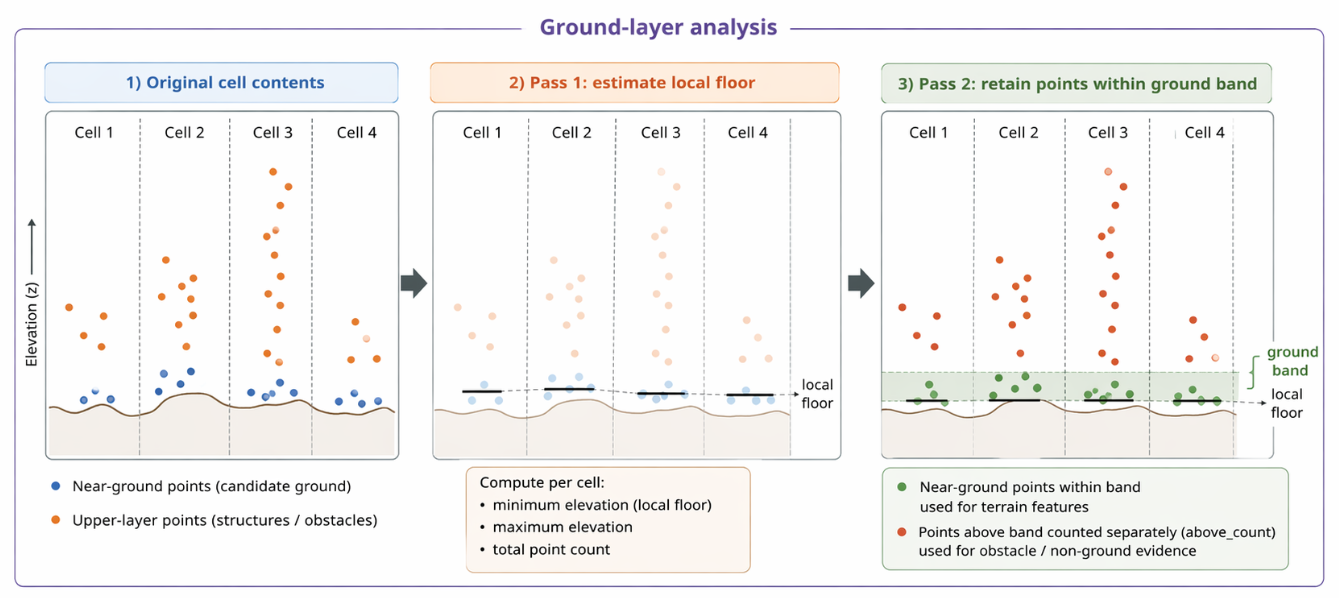
\includegraphics[width=0.9\linewidth]{figures/chizou/groundlayer.png}}
    \caption{Two-pass ground-layer extraction.}
    \label{fig:chizou-groundlayer}
\end{figure}

Based on the extracted near-ground layer, the pipeline computes local features, including \texttt{mean\_z}, \texttt{elev\_diff}, \texttt{roughness}, \texttt{slope}, and \texttt{above\_count}. It then applies an observation quality gate to identify insufficiently observed regions. Cells that satisfy the minimum near-ground point count and local coverage requirements are treated as well observed, while the remaining cells are labelled as UNKNOWN.

For well-observed cells, the final hard block is constructed from \texttt{obstacle\_core}, \texttt{step\_edge}, and optional expansion zones. \texttt{obstacle\_core} represents distinct near-ground vertical obstacles, whereas \texttt{step\_edge} captures abrupt local height changes. Cells that are well observed but not included in the hard block are labelled EXPLORABLE. A simple cleanup step is finally applied to remove isolated cells and improve the continuity of the semantic map.

\subsubsection{Cost-Map Generation}
\label{subsec:chizou-costmap-generation}

After the semantic map has been generated, the programme proceeds to construct a continuous traversability cost map. The system only calculates continuous costs for EXPLORABLE cells and assigns the maximum cost to both UNKNOWN and BLOCKED cells. The cost map is constructed as a weighted combination of multiple normalised features, including slope, roughness, \texttt{elev\_diff}, and an obstacle proximity term derived from the distance transform~\cite{chen2022gpu}. In this way, the cost map not only preserves the discrete semantic boundaries but also represents the relative difficulty of traversal within passable regions.

\subsubsection{Representative Map Outputs and Implementation Evaluation}
\label{subsec:chizou-map-outputs}

Figure~\ref{fig:chizou-frame5d} shows the semantic map for scene \texttt{frame\_5\_D} and its corresponding traversability cost map. After preprocessing, the scene is represented on a $37 \times 30$ grid with a cell resolution of 0.05 m. The semantic map shows that UNKNOWN mainly occupies peripheral regions with limited observation, while EXPLORABLE appears near the sensor origin and BLOCKED is concentrated around obstacle boundaries and step-like edges. This distribution is consistent with the proposed observation-gated and step-edge-based classification design.

\begin{figure}[H]
    \centering
    \makebox[\linewidth][c]{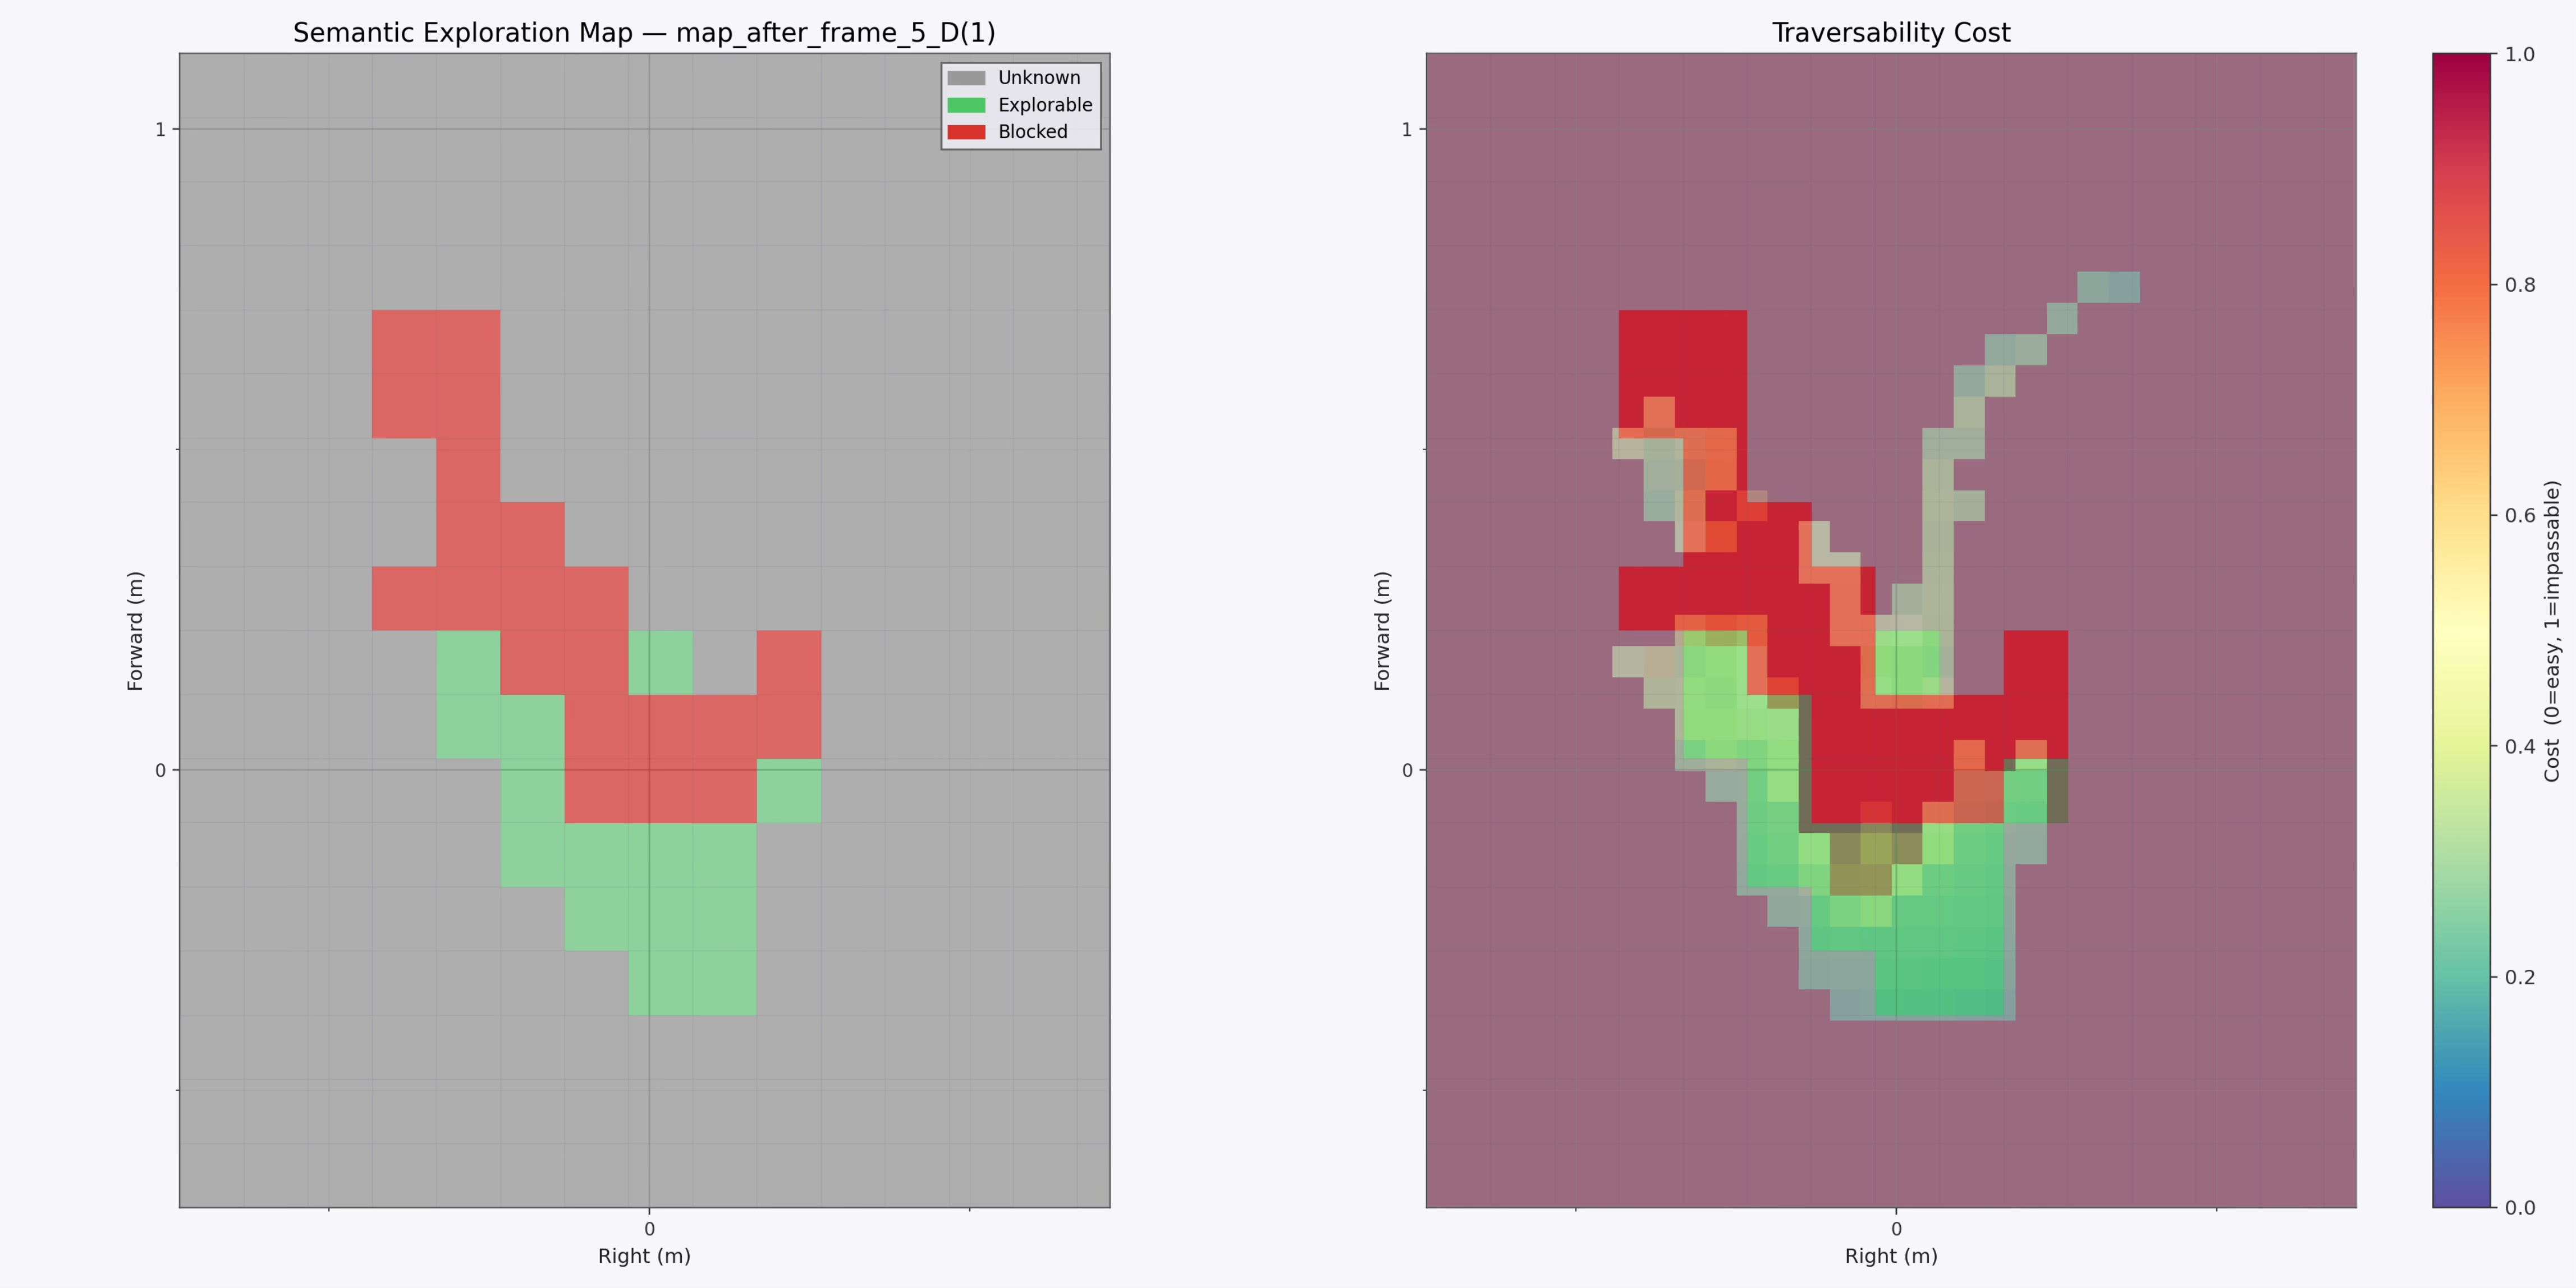
\includegraphics[width=0.9\linewidth]{figures/chizou/semantic_cost_frame5d.jpg}}
    \caption{Semantic exploration map and traversability cost map for scene \texttt{frame\_5\_D}.}
    \label{fig:chizou-frame5d}
\end{figure}

The corresponding cost map exhibits a smooth cost gradient within the EXPLORABLE region. Costs are lower in cells farther from BLOCKED areas and higher near obstacle boundaries. This behaviour is consistent with the proximity term derived from the distance transform.

Figure~\ref{fig:chizou-morecase} presents three additional semantic maps that illustrate the range of conditions in the test set.

\begin{itemize}
    \item Scene \texttt{frame\_6\_S} contains a larger proportion of valid near-ground observations and therefore a wider EXPLORABLE region.
    \item Scene \texttt{map (1)} shows a corridor-like layout, where BLOCKED is mainly concentrated along the side boundaries, leaving a continuous central passage.
    \item By contrast, scene \texttt{frame\_1\_D} represents a sparse and noisy case, in which most cells remain UNKNOWN.
\end{itemize}

These examples indicate that the pipeline preserves traversable structure when observations are sufficient, while remaining conservative when evidence is limited.

\begin{figure}[H]
    \centering
    \makebox[\linewidth][c]{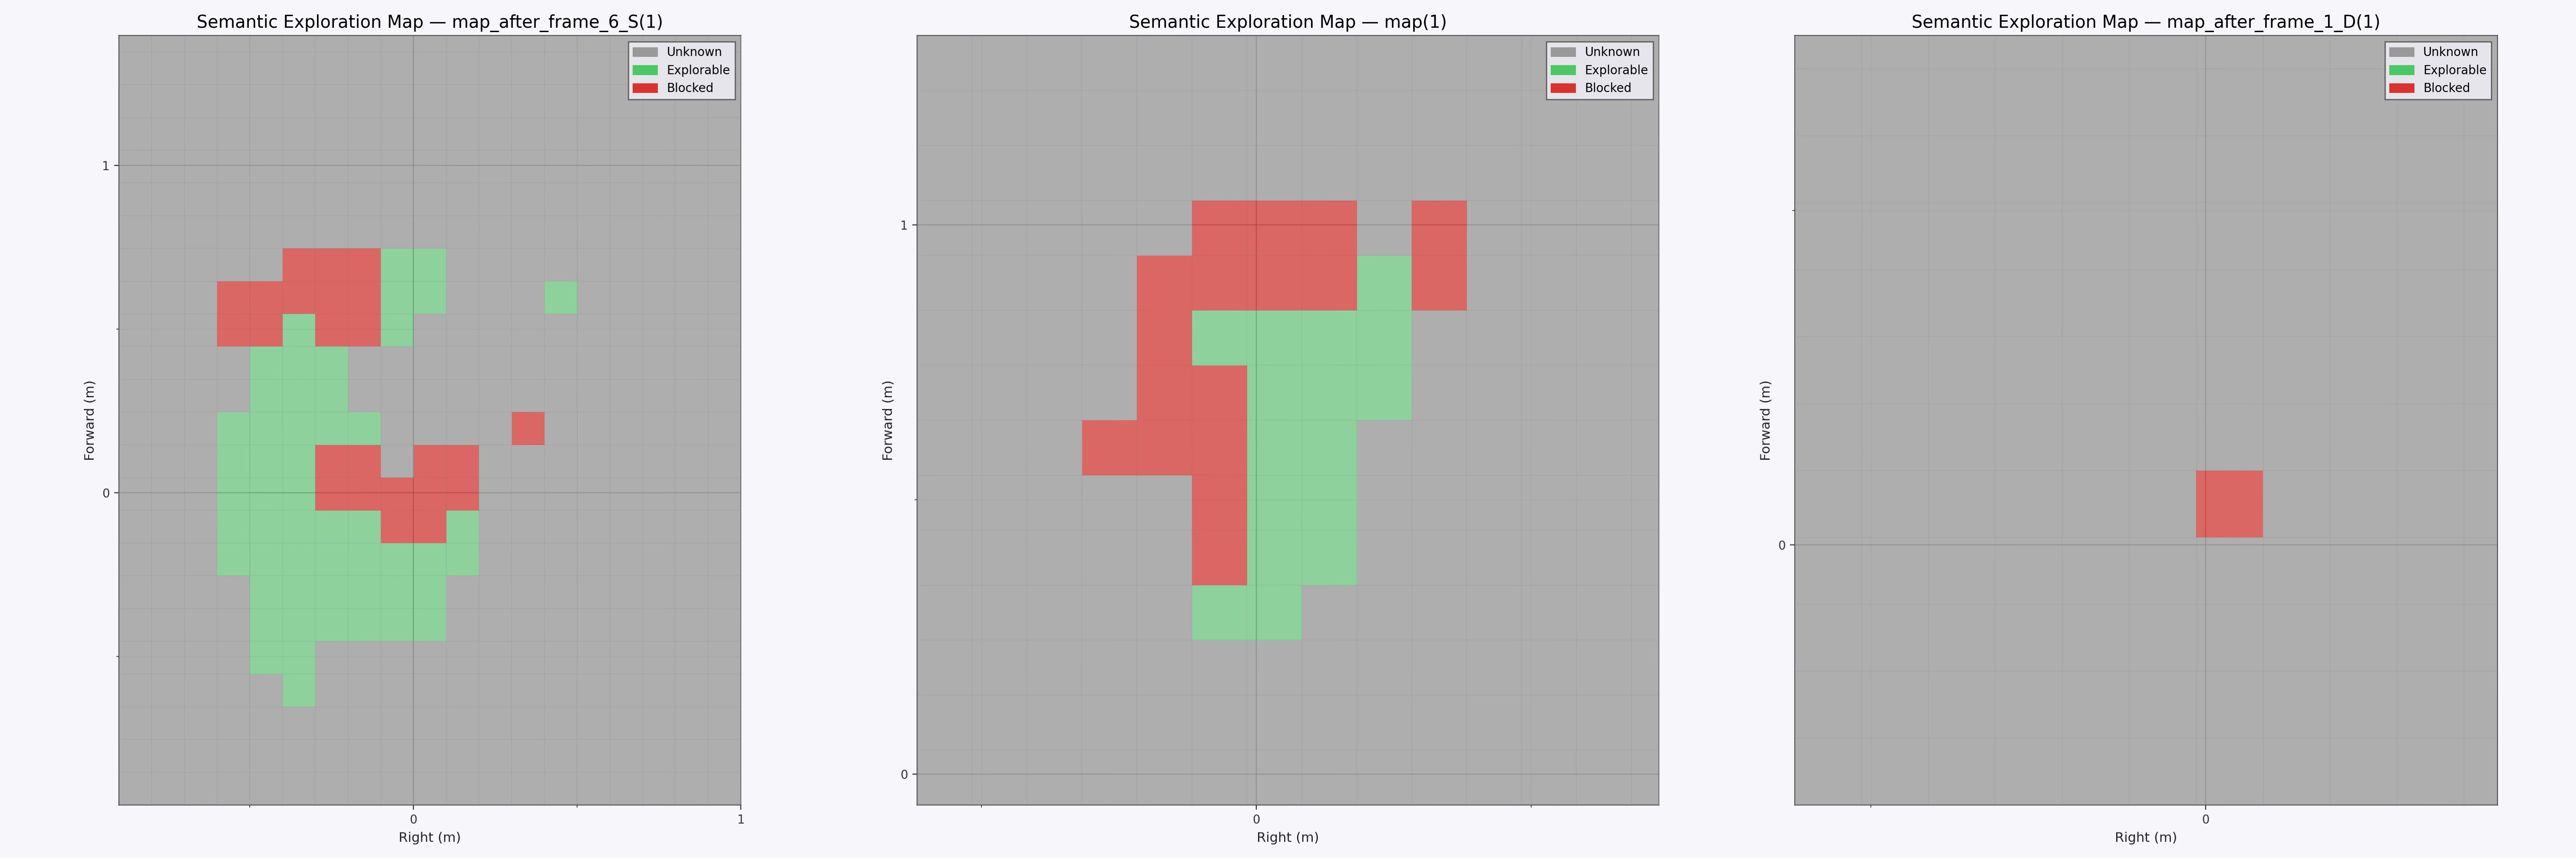
\includegraphics[width=0.9\linewidth]{figures/chizou/morecase.jpg}}
    \caption{Additional semantic-map examples from representative scenes in the test set.}
    \label{fig:chizou-morecase}
\end{figure}

\subsubsection{Quantitative Comparison and Design Analysis}
\label{subsec:chizou-quantitative-analysis}

\begin{table}[H]
    \centering
    \resizebox{\textwidth}{!}{%
    \begin{tabular}{lcccc}
        \toprule
        \textbf{Scene} & \textbf{Grid (H $\times$ W)} & \textbf{UNKNOWN \%} & \textbf{EXPLORABLE \%} & \textbf{BLOCKED \%} \\
        \midrule
        map(1)                & 29 $\times$ 28 & 81.90 & 13.92 & 4.19 \\
        map(3)                & 36 $\times$ 28 & 81.65 & 16.07 & 2.28 \\
        map\_after\_frame\_1\_D & 24 $\times$ 22 & 95.45 & 4.36  & 0.19 \\
        map\_after\_frame\_1\_S & 19 $\times$ 20 & 95.26 & 2.63  & 2.11 \\
        map\_after\_frame\_2\_D & 30 $\times$ 26 & 92.82 & 5.51  & 1.67 \\
        map\_after\_frame\_2\_S & 30 $\times$ 26 & 88.85 & 9.10  & 2.05 \\
        map\_after\_frame\_3\_D & 32 $\times$ 26 & 90.26 & 6.01  & 3.73 \\
        map\_after\_frame\_3\_S & 30 $\times$ 26 & 88.85 & 9.10  & 2.05 \\
        map\_after\_frame\_4\_D & 34 $\times$ 27 & 88.24 & 8.06  & 3.70 \\
        map\_after\_frame\_4\_S & 36 $\times$ 30 & 85.09 & 13.06 & 1.85 \\
        map\_after\_frame\_5\_D & 37 $\times$ 30 & 84.14 & 11.44 & 4.41 \\
        map\_after\_frame\_5\_S & 44 $\times$ 39 & 82.93 & 14.86 & 2.21 \\
        map\_after\_frame\_6\_S & 48 $\times$ 39 & 79.59 & 17.68 & 2.72 \\
        \midrule
        Mean (n=13)   & --- & 87.31 & 10.14 & 2.55 \\
        Median (n=13) & --- & 88.24 & 9.10  & 2.21 \\
        \bottomrule
    \end{tabular}%
    }
    \caption{Class distribution across the 13-scene test set under the default parameter setting.}
    \label{tab:chizou-class-dist}
\end{table}

Table~\ref{tab:chizou-class-dist} summarises the class distribution across the 13-scene test set under the default parameter setting. Across the dataset, UNKNOWN remains the dominant class, while EXPLORABLE and BLOCKED occupy relatively small proportions. This is consistent with the single-frame nature of monocular depth input, where only part of the environment is observed in each frame and the observation gate therefore retains a large proportion of cells as UNKNOWN. The limited size of the BLOCKED set indicates that the current pipeline does not over-label non-traversable areas when evidence is sparse.

\begin{table}[H]
    \centering
    \resizebox{\textwidth}{!}{%
    \begin{tabular}{ccccc}
        \toprule
        \textbf{traversable\_step\_height (m)} & \textbf{UNKNOWN \%} & \textbf{EXPLORABLE \%} & \textbf{BLOCKED \%} & \textbf{$\Delta$BLOCKED vs default} \\
        \midrule
        0.04             & 84.05 & 9.73  & 6.22 & $+1.81$ pp \\
        0.06             & 84.14 & 10.36 & 5.50 & $+1.09$ pp \\
        0.08 (default)   & 84.14 & 11.44 & 4.41 & ---        \\
        0.10             & 84.14 & 12.07 & 3.78 & $-0.63$ pp \\
        0.12             & 84.05 & 12.34 & 3.60 & $-0.81$ pp \\
        \bottomrule
    \end{tabular}%
    }
    \caption{Sensitivity of class distribution to \texttt{traversable\_step\_height} in scene \texttt{frame\_5\_D}.}
    \label{tab:chizou-step-height}
\end{table}

\begin{table}[H]
    \centering
    \resizebox{\textwidth}{!}{%
    \begin{tabular}{ccccc}
        \toprule
        \textbf{min\_step\_support} & \textbf{UNKNOWN \%} & \textbf{EXPLORABLE \%} & \textbf{BLOCKED \%} & \textbf{$\Delta$BLOCKED vs default} \\
        \midrule
        2             & 84.05 & 10.81 & 5.14 & $+0.73$ pp \\
        3 (default)   & 84.14 & 11.44 & 4.41 & ---        \\
        4             & 84.05 & 12.16 & 3.78 & $-0.63$ pp \\
        5             & 83.96 & 12.97 & 3.06 & $-1.35$ pp \\
        \bottomrule
    \end{tabular}%
    }
    \caption{Sensitivity of class distribution to \texttt{min\_step\_support} in scene \texttt{frame\_5\_D}.}
    \label{tab:chizou-min-step-support}
\end{table}

Table~\ref{tab:chizou-step-height} and Table~\ref{tab:chizou-min-step-support} show that increasing \texttt{traversable\_step\_height} or \texttt{min\_step\_support} leads to a monotonic decrease in the proportion of BLOCKED cells, while UNKNOWN remains largely unchanged. This suggests that these parameters mainly control the strictness of step-edge detection rather than the behaviour of the observation gate. By contrast, changing \texttt{min\_obs\_neighbours} has little effect on the final class distribution.

\begin{table}[H]
    \centering
    \begin{tabular}{cccc}
        \toprule
        \textbf{Configuration} & \textbf{UNKNOWN \%} & \textbf{EXPLORABLE \%} & \textbf{BLOCKED \%} \\
        \midrule
        Slope hard-block, $>15^{\circ}$ & 83.96 & 5.23  & 10.81 \\
        Slope hard-block, $>20^{\circ}$ & 83.96 & 5.77  & 10.27 \\
        Slope hard-block, $>30^{\circ}$ & 84.05 & 8.11  & 7.84  \\
        Slope hard-block, $>40^{\circ}$ & 84.05 & 9.46  & 6.49  \\
        Slope hard-block, $>50^{\circ}$ & 84.05 & 10.90 & 5.05  \\
        Slope as soft cost (current)    & 84.14 & 11.44 & 4.41  \\
        \bottomrule
    \end{tabular}
    \caption{Effect of reintroducing slope as a hard-blocking criterion in scene \texttt{frame\_5\_D}.}
    \label{tab:chizou-slope-ablation}
\end{table}

Table~\ref{tab:chizou-slope-ablation} further discusses the treatment of slope in the current design. When slope is reintroduced as a hard-blocking criterion, the proportion of BLOCKED cells increases substantially and the EXPLORABLE region is correspondingly reduced. This suggests that slope is highly sensitive to local discretisation and height noise in the present depth-derived point clouds and would therefore introduce excessive false positives if used as a hard block.

Overall, these results support the current design choice of reserving hard blocking for stronger geometric evidence, while retaining slope in the continuous cost map as a soft penalty.

\subsubsection{Discussion of Robustness and Limitations}
\label{subsec:chizou-robustness-limitations}

These tests show that the current method is capable of generating 2D maps from single-frame depth-derived point clouds. The UNKNOWN regions are primarily influenced by the quality of the observations, and the BLOCKED regions mainly appear near the boundaries of obstacles and the edges of steps. These results are consistent with the expected design. However, as this method was evaluated using only 13 sets of monocular depth point clouds and did not employ external ground truth, the analysis focuses on internal consistency rather than absolute accuracy. In sparse or noisy scenes, large areas of UNKNOWN may remain, which may require recalibration of the parameters.



\section{Repositories Related to This Work}

Zhuyu Dong:
\begin{itemize}
    \item \textbf{Project code repositories:}
    
    \url{https://github.com/SlamRobotV3/RobotESP32.git}
    
    \url{https://github.com/SlamRobotV3/ControlUtils.git}
    
    \url{https://github.com/SlamRobotV3/2D_map.git}

    \url{https://github.com/SlamRobotV3/SUM.git}
    
    \item \textbf{Report writing repository:}
    
    \url{https://github.com/xzzc666/project-2-final-report.git}
\end{itemize}

Junjie Ouyang:
\begin{itemize}
    \item \textbf{Project code repository:}
    
    \url{https://github.com/SlamRobotV3/Image_to_3D}
    
    \item \textbf{Report writing repository:}
    
    \url{https://github.com/nuanzhi6666/writing}
\end{itemize}

Qingzhou Zhang:
\begin{itemize}
    \item \textbf{Project code repository:}
    
    \url{https://github.com/SlamRobotV3/Merging.git}
\end{itemize}

Chi Zou:
\begin{itemize}
    \item \textbf{Project code repository:}
    
    \url{https://github.com/SlamRobotV3/2D-map-creation.git}
\end{itemize}

Weijie Chen:
\begin{itemize}
    \item \textbf{Project code repository:}
    
    \url{https://github.com/SlamRobotV3/pathplan.git}
    
    \item \textbf{Report writing repository:}
    
    \url{https://github.com/ntjj6/final-report}
\end{itemize}

\section{AI Assistance Statement}

OpenAI's GPT-5.4 and GPT-5.3 Codex were used as auxiliary tools during the development of this project and the preparation of this report. Their main uses included code assistance during implementation, support for idea expansion and organization during project planning, and assistance with translation, grammatical polishing, and length reduction during report writing. However, the main technical ideas, system design decisions, implementation work, and core content of the project were developed by the author. Drafts and iteration details related to the writing process can be examined through the commit history of the repositories listed in the previous section.



\end{document}
